\documentclass{article}

\usepackage[english]{babel}
\usepackage{amsmath}
\usepackage{amssymb}
\usepackage{amsthm}
\usepackage{blkarray}
\usepackage[font=small]{caption}
\usepackage{cite}
\usepackage{graphicx}

% ---- Propositions, lemmas, defintions... ---- %

\newtheorem{algorithm}{Algorithm}
\newtheorem{corollary}{Corollary}
\newtheorem{definition}{Definition}
%\newtheorem{example}{Example}
\newtheorem{lemma}{Lemma}
\newtheorem{proposition}{Proposition}
%\newtheorem{remark}{Remark}


% ---- Special environments (examples and remarks) ---- %

\newcounter{examplecounter}
\newenvironment{example}
{\small\vspace{0.5\baselineskip}
  \refstepcounter{examplecounter}%
  \noindent\textbf{Example \arabic{examplecounter}.}%
}{\vspace{-0.2\baselineskip}\begin{center}%
  $\star$\end{center}\vspace{0.5\baselineskip}}

\newcounter{remarkcounter}
\newenvironment{remark}
{\small\it\vspace{0.5\baselineskip}
  \refstepcounter{remarkcounter}%
  \noindent\textbf{Remark \arabic{remarkcounter}.}%
}{\vspace{0.5\baselineskip}}

\newenvironment{inset}
{\vspace{0.5\baselineskip}\begin{center}}
{\end{center}\vspace{0.5\baselineskip}}


% ---- Macros ---- %

\newcommand{\smA}{\scriptstyle{A}}
\newcommand{\smC}{\scriptstyle{C}}
\newcommand{\smD}{\scriptstyle{D}}
\newcommand{\smE}{\scriptstyle{E}}
\newcommand{\smG}{\scriptstyle{G}}
\newcommand{\smI}{\scriptstyle{I}}
\newcommand{\smS}{\scriptstyle{S}}
\newcommand{\smT}{\scriptstyle{T}}
\newcommand{\smDELz}{\scriptstyle{\Delta_0}}
\newcommand{\smDELs}{\scriptstyle{\Delta_*}}


%---------------------------------------------------------------

\title{Analytic combinatorics for bioinformatics I:
seeding methods}
\author{
\textsc{Guillaume Filion and Eduard Valera Zorita} \\ [1ex]
\normalsize CRG, Barcelona
}
\date{\today}

%---------------------------------------------------------------
%---------------------------------------------------------------


\begin{document}

\maketitle

\begin{abstract}
The abstract will come later.
\end{abstract}


%---------------------------------------------------------------
%---------------------------------------------------------------

\section{Introduction}

High throughput sequencing is changing the face of biology. More data is
of course better, but recently, technical improvements have started to
outpace the progress of algorithms. When the problems are too large,
one has to replace exact algorithms by heuristics that are much faster,
but do not guarantee to return the right result. Good heuristics are all
about understanding the input data. With the right data model, we can
calculate the risk of not returning the right answer and adjust the
algorithm to achieve more precision or more speed. When the data is poorly
understood, heuristics may be slow or inefficient for unknown reasons.

A particular area of bioinformatics where heuristics have been in use for
a long time is the field of sequence alignment. Computing the best
alignment between two sequences is carried out by dynamic programming in
time $O(mn)$, where $m$ and $n$ are the sequence lengths. When at least
one of the sequences is long (\textit{e.g.} a genome), this is prohibitive
and heuristics are required.

The most studied heuristics for sequence alignment are called seeding
methods. In a nutshell, the idea is to search short regions of the two
sequences that are very similar and use them as candidates to anchor the
dynamic programming alignment, which is performed only locally
\textit{i.e.} between subsequences of the input. These short regions of
high similarity are called ``seeds''. The benefit of the approach is that
seeds can be found in short time. The risk is that they may not exist,
even if the input sequences are similar.


\begin{figure}[h]
\centering
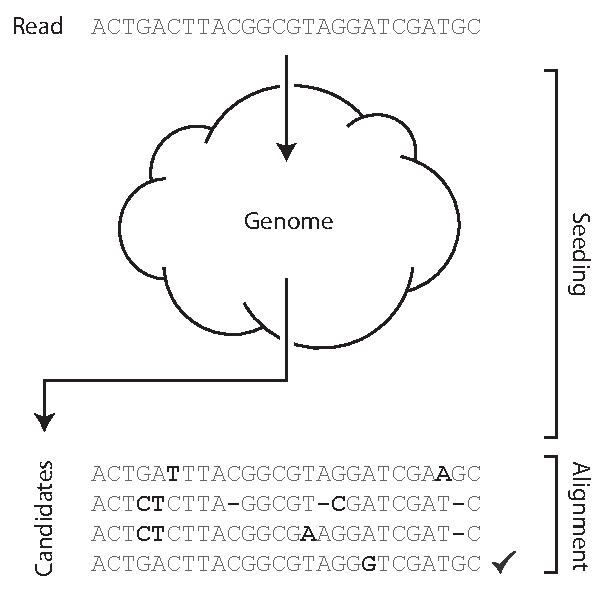
\includegraphics[scale=.9]{cloud_genome.pdf}
\caption{\textbf{Seeding heuristic in the mapping problem}. The sequencing
read belongs to an unknown portion of the genome; the task is to find its
original sequence (and usually its location). Because of possible read
errors, the read may not be identical to the original sequence. Most
algorithms feature a seeding stage and an alignment stage. The purpose of
seeding is to output a short list of candidate sequences, that of
alignment is to determine which is the best. Seeding is a heuristic
because it does not guanrantee that the overall best sequence is in the
list of candidates.}
\label{fig:cloud_genome}
\end{figure}


This strategy was most famously implemented in BLAST for the purpose of
finding local homology between proteins. By working out an approximate
distribution of the identity score for the seeds, the authors were able to
calibrate the BLAST heuristic very accurately in order to gain speed. The
algorithm always performs the minimum amount of work for a desired
confidence level.

Seeding methods are also heavily used in the mapping problem (see
figure~\ref{fig:cloud_genome}), where the original sequence of a read must
be found in a reference genome. The dicovery of indexing methods based on
the Burrows-Wheeler transform was instrumental to develop short read
mappers such as BWA and Bowtie. With such indexes, one can know the number
of occurrences of a substring in a genome in time independent of the
genome size. This yields a powerful seeding strategy whereby all the
substrings of the read are queried in the genome. The main limitation is
that the seeds must have exactly the same sequence in the read as in the
genome.

The heuristic should be calibrated from the probability that a seed of
given length can be found in the read, but this problem has not been fully
solved. The answer depends on the types and frequencies of errors, which
are often context-dependent. Overall, the lack of theoretical framework to
model seeding probabilities is halting progress on this line of research.

Here we solve this problem for arbitrary error models using the powerful
theory of analytic combinatorics. This field of research was initiated by
Donlad Knuth in the early days of algorithmics, and later developed by
Robert Sedgewick and Philippe Flajolet. The theory is now mature and used
to tackle many problems outside the analysis of algorithms. However, it
has not yet been realized how useful it can be for bioinformatics.

This document is predominantly written for bioinformaticians and people
with a working knowledge of sequencing technologies and their applications.
Accordingly, the focus will be on explaining the mathematical concepts,
rather than the technological aspects. Also, our goal here is not to push
the boundaries of analytic combinatorics, but to explain how its simplest
concepts are useful to solve common problems in bioinformatics. We have
opted for simplicity, to the detriment of generality and rigor. The
results presented here are only a basic introduction to analytic
combinatorics; the field is currently much more advanced and we refer the
interested to the original literature.

\section{Elements of analytic combinatorics}
\label{sec:anal}

\subsection{Weighted generating functions}
\label{subsec:WGF}


% ---------------  Definition of WGFs  --------------- %
\begin{definition}
\label{def:GF}
Let $\mathcal{A}$ be a set of combinatorial objects characterized by a
size and a weight. The \textbf{weighted generating function} of
$\mathcal{A}$ is defined as

\begin{equation}
\label{eq:GF1}
A(z) = \sum_{a \in \mathcal{A}} w(a) z^{|a|},
\end{equation}
where $|a|$ and $w(a)$ denote the \textbf{size} and \textbf{weight} of the
object $a$, respectively. Expression (\ref{eq:GF1}) also defines a
sequence $(a_k)_{k \geq 0}$ such that 

\begin{equation}
\label{eq:GF2}
A(z) = \sum_{k=0}^\infty a_k z^k.
\end{equation}

By definition $a_k = \sum_{a \in A_k}w(a)$, where $A_k$ is the class of
objects of size $k$ in $\mathcal{A}$. The number $a_k$ is called the total
weight of objects of size $k$.
\end{definition}
% ---------------------------------------------------- %

\begin{remark}
Expression (\ref{eq:GF2}) shows that the terms $a_k$ are the coefficients
of the Taylor series of $A(z)$.
\end{remark}

\begin{remark}
\label{rem:noweight}
If the weight of every object $a \in \mathcal{A}$ is $1$, then $A(z)$ is
called a \emph{simple generating function}, and in expression
(\ref{eq:GF2}) $a_k = |\mathcal{A}_k|$ is the number of objects of size
$k$ in $\mathcal{A}$.
\end{remark}

\begin{remark}
Typical combinatorial objects include binary trees, permutations,
derangements, multisets \textit{etc}., but here we will focus exclusively
on sequences of letters from finite alphabets. In what follows, the reader
can think of ``objects'' as ``finite sequences of letters''.
\end{remark}

Expressions (\ref{eq:GF1}) and (\ref{eq:GF2}) are of course equivalent.
Depending on the context, we will use one or the other.

\begin{example}
\label{ex:BABA}
Let $\mathcal{A} = \{a\}$ and $\mathcal{B} = \{b\}$ be alphabets with a
single letter (of size $1$). Assume $w(a) = p$ and $w(b) = q$. The
weighted generating functions of $\mathcal{A}$ and $\mathcal{B}$ are then
$A(z) = pz$ and $B(z) = qz$, respectively.
\end{example}

The motivation for definition~\ref{def:GF} is that operations on
combinatorial objects translate into operations on their weighted
generating functions. With the methods detailed below, we will obtain the
weighted generating functions of elaborate combinatorial objects from
simple ones. Using equation (\ref{eq:GF2}), we will extract the weight or
probability of objects of size $k$ from such weighted generating
functions.

This approach is counter-intuitive at first, but propositions~\ref{th:HBT}
and \ref{th:ass} below will show how we can compute probabilities that
are inacessible to more frontal approaches.

Let us start with the most straightforward ways to obtain new weighted
generating functions: additions and multiplications. If $A(z)$ and $B(z)$
are the weighted generating functions of two mutually exclusive sets
$\mathcal{A}$ and $\mathcal{B}$, the weighted generating function of
$\mathcal{A} \cup \mathcal{B}$ is $A(z) + B(z)$, as appears immediately
from expression (\ref{eq:GF1}).

\begin{example}
\label{ex:AUB}
With the definitions of example~\ref{ex:BABA}, the weighted generating
function of the alphabet $\mathcal{A} \cup \mathcal{B}= \{a,b\}$ is $pz +
qz = A(z) + B(z)$.
\end{example}

Size and weight can be defined for pairs of objects in $\mathcal{A} \times
\mathcal{B}$ as $|(a,b)| = |a| + |b|$ and $w(a,b) = w(a)w(b)$. In other
words the sizes are added and the weights are multiplied.  With this
convention, the weighted generating function of the Cartesian product
$\mathcal{A} \times \mathcal{B}$ is $A(z)B(z)$. This simply follows from
expression (\ref{eq:GF1}) and

\begin{equation*}
A(z)B(z) =
\sum_{a\in \mathcal{A}}w(a)z^{|a|} \sum_{b\in \mathcal{B}}w(b)z^{|b|}
= \sum_{(a,b) \in \mathcal{A} \times \mathcal{B}} w(a)w(b)z^{|a|+|b|}.
\end{equation*}

\begin{example}
With the definitions of example~\ref{ex:BABA}, $\mathcal{A}^2 = \{(a,a)\}$
contains a single pair of letters, with size $2$ and weight $p^2$. Its
weighted generating function is $p^2z^2 = A(z)^2$.
\end{example}


\begin{example}
Still with the definitions of example~\ref{ex:BABA}, $(\mathcal{A} \cup
\mathcal{B})^2$ contains the four pairs of letters $(a,a)$, $(a,b)$,
$(b,a)$ and $ (b,b)$. They have size $2$ and respective weight $p^2$,
$pq$, $qp$, and $q^2$, so the weighted generating function of
$(\mathcal{A} \cup \mathcal{B})^2$ is $(p^2+2pq+q^2)z^2 =
\big(A(z)+B(z)\big)^2$.
\end{example}


We can further extend the definition of size and weight to any finite
Cartesian product in the same way. The sizes are always added and the
weights are always multiplied. The generating function of a cartesian
product then comes as the product of their generating functions. This
allows us to construct finite sequences of objects.

\begin{example}
\label{ex:sequences}
With the definitions of example~\ref{ex:BABA}, $\mathcal{A}^k = \{(a, a,
\ldots, a)\}$ contains a single $k$-tuple of letters, with size $k$ and
weight $p^k$, so its weighted generating function is $p^kz^k$. Since the
sets $\mathcal{A}, \mathcal{A}^2, \mathcal{A}^3,\ldots$ are mutually
exclusive, the weighted generating function of their union is

\begin{equation*}
pz + p^2z^2 + p^3z^3 + \ldots
\end{equation*}

This infinite Taylor series can be expressed as a simple function. For any
$k \geq 1$, $(1-pz) \big(pz + (pz)^2 + \ldots + (pz)^k \big) =
pz-(pz)^{k+1}$.  If $|z| < 1/p$, the term $(pz)^{k+1}$ vanishes as $k$
increases. So the weighted generating function of $\cup_{k\geq1}
\mathcal{A}^k$ is defined for $|z| < 1/p$ and is equal to

\begin{equation*}
pz + (pz)^2 + (pz)^3 + \ldots = \frac{pz}{1-pz}.
\end{equation*}
\end{example}

Example~\ref{ex:sequences} is fundamental. It can be generalized to any
set $\mathcal{A}$ of combinatorial objects.

\begin{proposition}
\label{th:sequences1}
Let $\mathcal{A}$ be a set with weighted generating function $A(z)$. The
weighted generating function of $\mathcal{A}^+ = \cup_{k=1}^\infty
\mathcal{A}^k$, called the set of \textbf{non-empty sequences} of elements
of $\mathcal{A}$ is defined for $|A(z)| < 1$ and is equal to

\begin{equation*}
\frac{A(z)}{1-A(z)}.
\end{equation*}
\end{proposition}

\begin{proof}
For $k \geq 1$, the weighted generating function of $\mathcal{A}^k$ is
$A(z)^k$. Since the sets $\mathcal{A}^k$ are mutually exclusive, the
weighted generating function of their union is $A(z) + A(z)^2 + \ldots =
A(z) / (1-A(z))$, provided $|A(z)| < 1$.
\end{proof}

We introduce the \textbf{empty object} $\varepsilon$, which has size $0$
and weight 1. Its weighted generating function is thus $1$. By convention,
we define the zeroth power of a combinatorial set $\mathcal{A}$ as
$\mathcal{A}^0 = \{\varepsilon\}$. With this definition, we can state a
variant of the previous proposition.

\begin{proposition}
\label{th:sequences2}
Let $\mathcal{A}$ be a set with weighted generating function $A(z)$. The
weighted generating function of $\mathcal{A}^* = \cup_{k=0}^\infty
\mathcal{A}^k$, called the set of \textbf{sequences} of elements of
$\mathcal{A}$ is defined for $|A(z)| < 1$ and is equal to

\begin{equation*}
\frac{1}{1-A(z)}.
\end{equation*}
\end{proposition}

\begin{proof}
$\mathcal{A}^* = \{\varepsilon\} \cup \mathcal{A}^+$. By proposition
\ref{th:sequences1}, the weighted generating function is $1 +
A(z)/(1-A(z)) = 1/(1-A(z))$, provided $|A(z)| < 1$.
\end{proof}


\begin{remark}
\label{rem:no_seq_epsilon}
These expressions are not defined for $A(z) = 1$, \textit{i.e.} when
$\mathcal{A}$ contains only the empty object. In other words, one cannot
construct sequences of empty ojects. More generally, we will always assume
that the sets used to construct sequences do not contain the empty object
$\varepsilon$. Otherwise, $\varepsilon$ is present in each
$\mathcal{A}^k$ and they are not mutually exclusive.
\end{remark}

\begin{remark}
If $|A(z)| > 1$, the function  $A(z)/(1-A(z))$ is well defined but the
series $A(z) + A(z)^2 + \ldots$ does not converge. This is not a problem,
as relation (\ref{eq:GF2}) does not need to hold for every $z$. However,
in what follows we will always assume that it does. In other words, we
will always assume that $|z|$ is smaller than the radius of convergence of
the weighted generating function of interest.
\end{remark}


It is important to insist that the expression ``sequences of'' refers to
the set $\mathcal{A}^*$ and not to $\mathcal{A}^+$, \textit{i.e.} the
empty object $\varepsilon$ is a sequence of anything. For clarity, we will
systematically use the expression ``non-empty sequences of'' when
$\varepsilon$ is excluded.

\begin{example}
\label{ex:AUB+}
Following the definitions of example~\ref{ex:BABA}, $(\mathcal{A} \cup
\mathcal{B})^*$ is the set of sequences of $a$'s and $b$'s. By
proposition~\ref{th:sequences2} and example~\ref{ex:AUB}, the weighted
generating function of this set is

\begin{equation*}
\frac{1}{1-(p+q)z}.
\end{equation*}

The function $1 / (1-(p+q)z)$ is just a compact representation of the
infinite series $1, (p+q), (p+q)^2, (p+q)^3, \ldots$ It thus carries all
the information about the total weights of the sequences of any size. If
$p = q = 1$, \textit{i.e.} if we count the total amount of sequences with
simple generating functions (see remark~\ref{rem:noweight}), we obtain
$1/(1-2z) = 1+ 2z + 4z^2 + 8z^3 + 16z^4 + \ldots$ meaning that there are
$2^k$ sequences of size $k$. If $p$ and $q$ are the respective
probabilities of ocurrence of $a$ and $b$, with $p + q \leq 1$, then the
equality $1 / (1-(p+q)z) = 1+ (p+q)z + (p+q)^2z^2 + (p+q)^3z^3 + \ldots$
means that the probability that a sequence of size $k$ contains only $a$'s
and $b$'s is $(p+q)^k$.
\end{example}

These simple examples are better solved by intuition. However, we will
soon see that analytic combinatorics allows us to solve a wider range of
problems.




%%%%%%%%%%%%%%%%% Transfer matrices %%%%%%%%%%%%%%%%%

\subsection{Sequences and transfer matrices}
\label{subsec:TransMat}

In many combinatorial applications, one needs to count the sequences where
a pattern does not occur, or where some symbols may not follow each other.
A convenient way to find the weighted generating functions of such
sequences is to encode this information in so-called ``transfer
matrices''. We will illustrate the process with an example from biology.

In many animal genomes, DNA methylation can only occur on the dinucleotide
\texttt{CG}. Because of this property, it is interesting to count the
sequences that have no \texttt{CG}. Sequences without \texttt{CG} can be
thought of as walks on a directed graph with restricted transitions.
Nucleotides are represtend as nodes, and edges indicate that the
nucleotide at the tip can follow the nucleotide at the base. Sequences
without \texttt{CG} correspond to walks on a complete graph where the edge
from \texttt{C} to \texttt{G} is removed (see
figure~\ref{fig:CG_transitions}).

\begin{figure}[h]
\centering
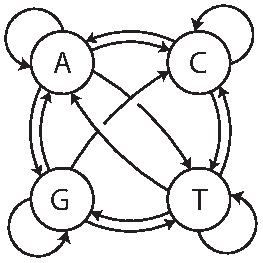
\includegraphics[scale=0.9]{CG_transitions.pdf}
\caption{\textbf{Graph representation of sequences of nucleotides without
\texttt{CG}}. A sequence without \texttt{CG} is equivalent to a walk on
this graph. All the transitions are allowed, except \texttt{C} to
\texttt{G}.}
\label{fig:CG_transitions}
\end{figure}

The same graph can also be represted as an adjacency matrix $M$, where a
$1$ at position $(i,j)$ indicates that there is an edge from node $i$ to
node $j$, and a $0$ indicates that there is no edge. For instance, the
adjacency matrix of the graph of figure~\ref{fig:CG_transitions} is

\begin{equation*}
M = 
\begin{blockarray}{ccccc}
     & \smA & \smC & \smG & \smT \\
\begin{block}{c[cccc]}
\smA & 1 & 1 & 1 & 1 \\
\smC & 1 & 1 & 0 & 1 \\
\smG & 1 & 1 & 1 & 1 \\
\smT & 1 & 1 & 1 & 1 \\
\end{block}
\end{blockarray}.
\end{equation*}

The main advantage of the adjacency matrix representation is that the
powers of $M$ give an analytical way to count the walks on the graph. The
entry of $M^n$ at position $(i,j)$ is the number of walks of $n$ steps
that start with node $i$ and end with node $j$. So we can count
sequences without \texttt{CG} by computing the successive powers of the
adjacency matrix $M$ above.

The same idea can be used to find the weighted generating function of
sequences of combinatorial objects. We specify the internal structure of
sequences by a ``transfer graph'', where the edges represent classes of
combinatorial objects.

\begin{definition}
\label{def:transfermat}
A \textbf{transfer graph} is a directed graph whose edges are weighted by
generating functions. In addition, a transfer graph must contain a head
vertex with only outgoing edges, and a tail vertex with only incoming
edges. The graph can be represented as a matrix called a \textbf{transfer
matrix}.
\end{definition}

Following the edges of a transfer graph from the head vertex to the tail
vertex describes a sequence of combinatorial objects. The associated
weighted generating function is the product of the functions labelling the
edges (thus an absent edge is associated to the function $0$).

Transfer graphs have the general structure below. The head vertex is
represented as an open circle and the tail vertex as a closed circle. The
edge labelled $\psi(z)$, from the head vertex to the tail vertex
represents additional sequences. Typically, $\psi(z) = 1$, as the only
sequence that needs to be added explicitly is the empty object
$\varepsilon$.

\begin{inset}
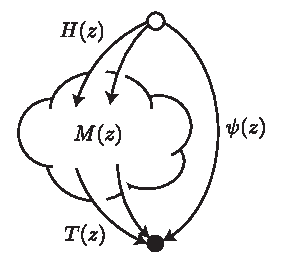
\includegraphics[scale=1.0]{cloud.pdf}
\end{inset}

The ``body'' of the graph, represented as a cloud, contains the remaining
$m$ vertices. $M(z)$ is the $m \times m$ matrix representation of the
corresponding sub-graph. $H(z)$ is a vector of $m$ weighted generating
functions associated with the $m$ edges from the head vertex to the body
of the graph, and $T(z)$ is a vector of $m$ weighted generating functions
associated with the edges from the body of graph to the tail vertex.
$H(z)$ and $T(z)$ are called the ``head'' and ``tail'' vectors,
respectively.

\begin{remark}
Transfer graphs are reminiscent of deterministic finite automata (DFA).
The initial and accept states of a DFA correspond to the head and tail
vertices of a transfer graph. The alphabet of a DFA corresponds to the
combinatorial objects that can be concatenated (or to their weighted
generating functions) and the transition function corresponds to the
transfer matrix. We will not make further use of this analogy in this
document.
\end{remark}

\begin{definition}
The \textbf{sequences generated by a transfer matrix} correspond to the
paths from the head vertex to the tail vertex of the associated tranfer
graph.
\end{definition}

\begin{example}
\label{ex:TMAz}
Let $\mathcal{A}$ be a class of combinatorial objects with weighted
generating function $A(z)$. Sequences of objects from $\mathcal{A}$ can be
thought of as walks on the graph below.

\begin{inset}
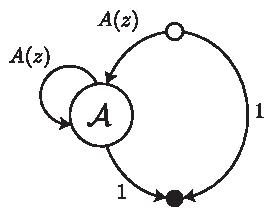
\includegraphics[scale=1.0]{A.pdf}
\end{inset}

The edge from the vertex $\mathcal{A}$ to the tail vertex marks the end of
the sequence, by appending a final empty object $\varepsilon$ with weight
$1$. The transfer matrix of this graph is the $3 \times 3$ matrix

\begin{equation*}
M_*(z) =
\begin{blockarray}{cccc}
     & \; \circ & \mathcal{A} & \bullet \; \\
\begin{block}{c[ccc]}
\circ       &  \; 0  & A(z) & 1 \; \\
\mathcal{A} &  \; 0  & A(z) & 1 \; \\
\bullet     &  \; 0  &  0   & 0 \; \\
\end{block}
\end{blockarray}.
\end{equation*}

The head vector $H(z)$ has dimension $1$ and is equal to $A(z)$. The tail
vector $T(z)$ also has dimension $1$ and is equal to $1$. $M(z)$, the
matrix of the body of the graph is the $1 \times 1$ matrix $[A(z)]$.
\end{example}


\begin{example}
\label{ex:TMABz}
Let $\mathcal{A}$ and $\mathcal{B}$ be mutually exclusive classes of
combinatorial objects with respective weighted generating function $A(z)$
and $B(z)$. Sequences of objects from $\mathcal{A}$ or $\mathcal{B}$ can
be thought of as walks on the graph below.

\begin{inset}
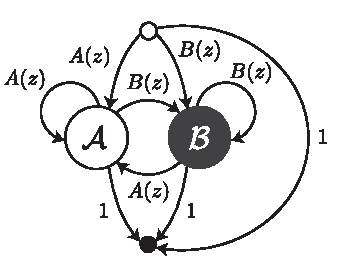
\includegraphics[scale=1.0]{AB_complete.pdf}
\end{inset}

The transfer matrix of this graph is the $4 \times 4$ matrix

\begin{equation*}
M_*(z) =
\begin{blockarray}{cccccc}
     & \; \circ & \mathcal{A} & \mathcal{B} & \bullet \; \\
\begin{block}{c[ccccc]}
\circ       &  \; 0  & A(z) & B(z) & 1 \; \\
\mathcal{A} &  \; 0  & A(z) & B(z) & 1 \; \\
\mathcal{B} &  \; 0  & A(z) & B(z) & 1 \; \\
\bullet     &  \; 0  &  0   & 0    & 0 \; \\
\end{block}
\end{blockarray}.
\end{equation*}

The head vector $H(z)$ has dimension $2$ and is equal to $(A(z),
B(z))^\top$. The tail vector $T(z)$ also has dimension $2$ and is equal to
$(1,1)^\top$. $M(z)$, the matrix of the body of the graph is the $2 \times
2$ matrix

\begin{equation*}
M(z) =
\begin{blockarray}{cccc}
     & \mathcal{A} & \mathcal{B} \\
\begin{block}{c[ccc]}
\mathcal{A} & A(z) & B(z) \\
\mathcal{B} & A(z) & B(z) \\
\end{block}
\end{blockarray}.
\end{equation*}
\end{example}


\begin{example}
\label{ex:TMAUBz}
With the assumptions of example~\ref{ex:TMABz}, sequences of objects from
$\mathcal{A}$ or $\mathcal{B}$ can also be thought of as walks on a the
graph below.

\begin{inset}
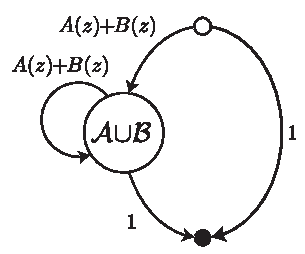
\includegraphics[scale=1.0]{AUB.pdf}
\end{inset}

Indeed, because $\mathcal{A}$ and $\mathcal{B}$ are mutually exclusive, we
know that the weighted generating function of $\mathcal{A}\cup\mathcal{B}$
is $A(z)+B(z)$. The transfer matrix of this graph is the $3 \times 3$
matrix

\begin{equation*}
M_*(z) =
\begin{blockarray}{cccc}
     & \; \circ & \mathcal{A}\cup\mathcal{B} & \bullet \; \\
\begin{block}{c[ccc]}
\circ                      &  \; 0  & A(z)+B(z) & 1 \; \\
\mathcal{A}\cup\mathcal{B} &  \; 0  & A(z)+B(z) & 1 \; \\
\bullet                    &  \; 0  &  0        & 0 \; \\
\end{block}
\end{blockarray}.
\end{equation*}

The head vector $H(z)$ has dimension $1$ and is equal to $A(z)+B(z)$.
The tail vector $T(z)$ also has dimension $1$ and is equal to
$1$. $M(z)$, the matrix of the body of the graph is the $1 \times
1$ matrix $M(z) = [A(z)+B(z)]$.
\end{example}

Examples~\ref{ex:TMABz} and \ref{ex:TMAUBz} show that the same class of
combinatorial sequences may be associated with multiple transfer matrices.
There are several ways to construct (and interpret) a weighted generating
function.

\begin{example}
\label{ex:TMAB0z}
Let $\mathcal{A}$ and $\mathcal{B}$ be mutually exclusive classes of
combinatorial objects with respective weighted generating function $A(z)$
and $B(z)$. Sequences of objects from $\mathcal{A}$ or $\mathcal{B}$ that
end with $\mathcal{B}$ but without two consecutive objects from
$\mathcal{B}$ can be thought of as walks on the graph below.

\begin{inset}
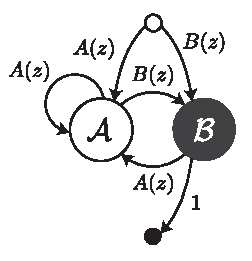
\includegraphics[scale=1.0]{AB_incomplete.pdf}
\end{inset}

The edge with weighted generating function $1$ from the head vertex to the
tail vertex is no longer present because the empty object $\varepsilon$
does not end with $\mathcal{B}$. The transfer matrix of this graph is the
$4 \times 4$ matrix

\begin{equation*}
M_*(z) =
\begin{blockarray}{cccccc}
     & \; \circ & \mathcal{A} & \mathcal{B} & \bullet \; \\
\begin{block}{c[ccccc]}
\circ       &  \; 0  & A(z) & B(z) & 0 \; \\
\mathcal{A} &  \; 0  & A(z) & B(z) & 0 \; \\
\mathcal{B} &  \; 0  & A(z) & 0    & 1 \; \\
\bullet     &  \; 0  &  0   & 0    & 0 \; \\
\end{block}
\end{blockarray}.
\end{equation*}

The head vector $H(z)$ has dimension $2$ and is equal to $(A(z),
B(z))^\top$. The tail vector $T(z)$ also has dimension $2$ and is equal to
$(0,1)^\top$. $M(z)$, the matrix of the body of the graph is the $2 \times
2$ matrix

\begin{equation*}
\begin{blockarray}{cccc}
     & \mathcal{A} & \mathcal{B} \\
\begin{block}{c[ccc]}
\mathcal{A} & A(z) & B(z) \\
\mathcal{B} & A(z) &  0   \\
\end{block}
\end{blockarray}.
\end{equation*}
\end{example}

Let us now return to sequences of nucleotides without \texttt{CG}. To
specify a transfer matrix, let us assume that \texttt{G}'s and
\texttt{C}'s occur with frequency $p/2$ and that \texttt{A}'s and
\texttt{T}'s occur with frequency $q/2$, where $q = 1-p$. The weighted
generating functions of the single nucleotides are thus $C(z) = G(z) =
pz/2$ and $A(z) = T(z) = qz/2$. With these definitions, the transfer
matrix of the graph shown in figure~\ref{fig:CG_transitions} is

\begin{align*}
M_*(z) &=
\begin{blockarray}{ccccccc}
     & \; \circ & \smA & \smC & \smG & \smT & \bullet \; \\
\begin{block}{c[cccccc]}
\circ    & \; 0 & A(z) & C(z) & G(z) & T(z) & 1 \; \\
\smA     & \; 0 & A(z) & C(z) & G(z) & T(z) & 1 \; \\
\smC     & \; 0 & A(z) & C(z) &  0   & T(z) & 1 \; \\
\smG     & \; 0 & A(z) & C(z) & G(z) & T(z) & 1 \; \\
\smT     & \; 0 & A(z) & C(z) & G(z) & T(z) & 1 \; \\
\bullet  & \; 0 &  0   &   0  &   0  &   0  & 0 \; \\
\end{block}
\end{blockarray} \\
&= 
z/2 
\begin{bmatrix}
0 & q & p & p & q & 1 \\
0 & q & p & p & q & 1 \\
0 & q & p & 0 & q & 1 \\
0 & q & p & p & q & 1 \\
0 & q & p & p & q & 1 \\
0 & 0 & 0 & 0 & 0 & 0
\end{bmatrix}.
\end{align*}

We still need to find the weighted generating function.
Proposition~\ref{prop:transfermatrices} below shows how this is done.

\begin{lemma}
\label{lemma:transfermatrices}
Given a transfer graph and its transfer matrix $M_*(z)$, the weighted
generating function of paths of $n$ segments from vertex $i$ to vertex $j$
is the entry of $M_*(z)^n$ at position $(i,j)$.
\end{lemma}

\begin{proof}
Proceed by induction. For $n = 1$, this is the definition of the transfer
matrix. Assume that the property holds for some $n \geq 1$. A path of
$n+1$ segments from vertex $i$ to vertex $j$ is a path of $n$ segments
from vertex $i$ to some vertex $k$, followed by a single segment from
vertex $k$ to vertex $j$. Using the induction hypothesis and taking the
union on all vertices $1 \leq k \leq m+2$, the weighted generating
function of such paths is

\begin{equation*}
\sum_{k = 1}^{m+2} \Big(M(z)^n\Big)_{[i,k]} \times M(z)_{[k,j]}
= \Big(M(z)^{n+1}\Big)_{[i,j]},
\end{equation*}
which concludes the proof by induction.
\end{proof}

\begin{proposition}
\label{prop:transfermatrices}
The weighted generating function of the sequences generated by a transfer
matrix $M_*(z)$ is the top right entry of the matrix $(I-M_*(z))^{-1}$,
assuming that all the eigenvalues of $M(z)$ have \textit{modulus} less
than $1$.
\end{proposition}

\begin{proof}
From lemma~\ref{lemma:transfermatrices}, the weighted generating function
is the top right entry of the matrix

\begin{equation*}
I + M_*(z) + M_*(z)^2 + M_*(z)^3 + \ldots
\end{equation*}

Observe that $(I-M_*(z)) \cdot (I+M_*(z)+M_*(z)^2+ \ldots + M_*(z)^n) =
I-M_*(z)^{n+1}$. If all the eigenvalues of $M(z)$ have \textit{modulus}
less than $1$, the right hand side converges to the identity matrix $I$ as
$n$ goes to infinity. This translates to

\begin{equation*}
I + M_*(z) + M_*(z)^2 + M_*(z)^3 + \ldots = (I-M_*(z))^{-1},
\end{equation*}
which concludes the proof.
\end{proof}


\begin{example}
Let us continue example~\ref{ex:TMAz} where

\begin{equation*}
M_*(z) =
\begin{blockarray}{cccc}
     & \; \circ & \mathcal{A} & \bullet \; \\
\begin{block}{c[ccc]}
\circ       &  \; 0  & A(z) & 1 \; \\
\mathcal{A} &  \; 0  & A(z) & 1 \; \\
\bullet     &  \; 0  &  0   & 0 \; \\
\end{block}
\end{blockarray}.
\end{equation*}

The weighted generating function of sequences of objects from
$\mathcal{A}$ is the top right entry of the matrix

\begin{equation*}
(I-M_*(z))^{-1} = \frac{1}{1-A(z)}
\begin{bmatrix}
1-A(z) & A(z) &   1    \\
 0     & 1    &   1    \\
 0     &  0   & 1-A(z) \\
\end{bmatrix}.
\end{equation*}

In other words, the weighted generating function of sequences of objects
from $\mathcal{A}$ is $1/(1-A(z)$, consistently with
proposition~\ref{th:sequences2}.
\end{example}

\begin{example}
\label{ex:WGFAUB}
Let us continue examples~\ref{ex:TMABz} and \ref{ex:TMAUBz}. The first
transfer matrix is

\begin{equation*}
\begin{blockarray}{cccccc}
     & \; \circ & \mathcal{A} & \mathcal{B} & \bullet \; \\
\begin{block}{c[ccccc]}
\circ       &  \; 0  & A(z) & B(z) & 1 \; \\
\mathcal{A} &  \; 0  & A(z) & B(z) & 1 \; \\
\mathcal{B} &  \; 0  & A(z) & B(z) & 1 \; \\
\bullet     &  \; 0  &  0   & 0    & 0 \; \\
\end{block}
\end{blockarray}.
\end{equation*}

Applying proposition~\ref{prop:transfermatrices}, the weighted generating
function of sequences of objects from $\mathcal{A}$ of $\mathcal{B}$ is
the top right entry of the matrix

\begin{equation*}
\frac{1}{1-A(z)-B(z)}
\begin{bmatrix}
1-A(z)-B(z) &    A(z)      &  B(z)  & 1 \\
     0      &   1-B(z)     &  B(z)  & 1 \\
     0      &    A(z)      & 1-A(z) & 1 \\
     0      &     0        &    0   & 1
\end{bmatrix}.
\end{equation*}

The second transfer matrix is

\begin{equation*}
\begin{blockarray}{cccc}
     & \; \circ & \mathcal{A}\cup\mathcal{B} & \bullet \; \\
\begin{block}{c[ccc]}
\circ                      &  \; 0  & A(z)+B(z) & 1 \; \\
\mathcal{A}\cup\mathcal{B} &  \; 0  & A(z)+B(z) & 1 \; \\
\bullet                    &  \; 0  &  0        & 0 \; \\
\end{block}
\end{blockarray}.
\end{equation*}

Applying proposition~\ref{prop:transfermatrices} again, the weighted
generating function of sequences of objects from from $\mathcal{A}$ or
$\mathcal{B}$ is the top right entry of the matrix

\begin{equation*}
\frac{1}{1-A(z)-B(z)}
\begin{bmatrix}
1-A(z)-B(z) & A(z)+B(z) & 1 \\
     0      &     1     & 1 \\
     0      &     0     & 1
\end{bmatrix}.
\end{equation*}

Both terms are equal to $1/(1-A(z)-B(z))$. This illustrates that there are
different ways to construct a sequence, some simpler than others.
\end{example}


We now introduce a simplified way to find weighted generating functions
from transfer matrices.

\begin{proposition}
\label{th:HBT}
Given a transfer matrix
\begin{equation*}
M_*(z) =
\begin{bmatrix}
0 & H(z)^\top & \psi(z) \\
0 & M(z) & T(z)    \\
0 &  0   &  0      \\
\end{bmatrix},
\end{equation*}
where $M(z)$ is a $m \times m$ matrix, $H(z)$ and $T(z)$ are vectors of
dimension $m$ and $\psi(z)$ has dimension $1$, the weighted generating
function of the sequences generated by $M_*(z)$ is

\begin{equation}
\psi(z) + H(z)^\top \cdot (I-M(z))^{-1} \cdot T(z),
\end{equation}
assuming that all the eigenvalues of $M(z)$ have \textit{modulus} less
than $1$.
\end{proposition}

\begin{proof}
We need to compute the top-right term of the matrix $(I-M_*(z))^{-1}$.
Using the matrix inversion formula with the cofactor matrix, this term is
equal to $(-1)^{m+2}C/\det(I-M_*(z))$, where $C$ is the determinant

\begin{equation*}
\begin{vmatrix}
-H(z)^\top  & -\psi(z) \\
I-M(z) & -T(z)    \\
\end{vmatrix}.
\end{equation*}

Developing $\det(I-M_*(z))$ along the first column and then along the last
row, we obtain $\det(I-M_*(z)) = (-1)^m\det(I-M(z))$. Developping $C$
along the first row and then along the last column, we obtain

\begin{equation*}
C = (-1)^m\psi(z)\det(I-M(z)) +
\sum_{i=1}^m\sum_{j=1}^m H_i(z) (-1)^{i+j} C_{i,j}(z) T_j(z),
\end{equation*}
where $C_{i,j}$ is the cofactor of $I-M(z)$ at position $(i,j)$. Using
once more the matrix inversion formula, we obtain

\begin{equation*}
\frac{(-1)^{m+2}C}{\det(I-M^*(z))} =
\psi(z) + H(z)^\top \cdot (I-M(z))^{-1} \cdot T(z).
\end{equation*}
\end{proof}


\begin{example}
Let us continue example~\ref{ex:TMAB0z} where

\begin{equation*}
M_*(z) =
\begin{blockarray}{cccccc}
     & \; \circ & \mathcal{A} & \mathcal{B} & \bullet \; \\
\begin{block}{c[ccccc]}
\circ       &  \; 0  & A(z) & B(z) & 0 \; \\
\mathcal{A} &  \; 0  & A(z) & B(z) & 0 \; \\
\mathcal{B} &  \; 0  & A(z) & 0    & 1 \; \\
\bullet     &  \; 0  &  0   & 0    & 0 \; \\
\end{block}
\end{blockarray}.
\end{equation*}


We have seen that $H(z) = (A(z), B(z))^\top$, $T(z) = (0,1)^\top$,
$\psi(z) = 0$ and

\begin{equation*}
M(z) =
\begin{blockarray}{cccc}
     & \mathcal{A} & \mathcal{B} \\
\begin{block}{c[ccc]}
\mathcal{A} & A(z) & B(z) \\
\mathcal{B} & A(z) &  0   \\
\end{block}
\end{blockarray}.
\end{equation*}

Using proposition~\ref{th:HBT}, the weighted generating function of the
sequences generated by $M_*(z)$ is 

\begin{equation*}
0 + [A(z) \; B(z)] \cdot \frac{1}{1-A(z)(1+B(z))}
\begin{bmatrix}
  1  &  B(z)  \\
A(z) & 1-A(z) \\
\end{bmatrix}
\cdot
\begin{bmatrix} 0 \\ 1 \end{bmatrix}
= \frac{B(z)}{1-A(z)(1+B(z))}.
\end{equation*}
\end{example}

We will sometimes represent transfer graphs as their bodies (associated
with the matrix $M(z)$), and specify separately $\psi(z)$, $H(z)$ and
$T(z)$. This will simplify the graphical representations, and using
proposition~\ref{th:HBT} instead of
proposition~\ref{prop:transfermatrices} will simplify the computations.

Now returning to sequences of nucleotides without \texttt{CG}, we have
$\psi(z) = 1$, $H(z) = (A(z),C(z),G(z),T(z))^\top =
(qz/2,pz/2,pz/2,qz/2)$, $T(z) = (1,1,1,1)^\top$, and

\begin{equation*}
M(z) = z/2
\begin{bmatrix}
q & p & p & q \\
q & p & 0 & q \\
q & p & p & q \\
q & p & p & q \\
\end{bmatrix}.
\end{equation*}

The inverse of $(I-M(z))^{-1}$ is

\begin{equation*}
\frac{1}{\lambda(z)} \left[
\begin{matrix}
(pz)^2+2qz+4   & 2pz        & pz(pz-2)   & 2qz                \\
-pqz^2+2qz     & -2(1+q)z+4 & 2pqz^2     & -pqz^2+2qz         \\
2qz            & 2pz        & -2(1+q)+4  & 2qz                \\
2qz            & 2pz        & pz(1-pz)   & (pz)^2 - 2(p+1) +4
\end{matrix}
\right]
\end{equation*}
where $\lambda(z) = 4 - 4z + (pz)^2$ is the determinant of $I-M(z)$. Now
applying proposition~\ref{th:HBT}, the weighted generating function of
sequences of nucleotides without \texttt{CG} comes out as

\begin{equation}
\label{eq:WGFnoCG}
1 + H(z)^\top \cdot (I-M(z))^{-1} \cdot T(z) = 
\frac{4}{4-4z+(pz)^2}.
\end{equation}

In this section we have seen that transfer matrices allow us to find the
weighted generating functions of potentially intricate sequences of
combinatorial objects. In the next section we will see how we can compute
the probabilities of such sequences from their weighted generating
function.




%%%%%%%%%%%%% The crown jewel proposition %%%%%%%%%%%%%

\subsection{Asymptotic estimates}
\label{sec:asest}

We know from expression (\ref{eq:GF2}) that we can recover the total
weight (\textit{i.e.} the probability) of objects of size $k$ from the
Taylor expansion of their weighted generating function. We will often need
to extract $a_k$ in expressions of the form $\sum_{k=1}^\infty a_k z^k$ so
we introduce the following symbol.

\begin{definition}
Let $W(z)$ be a weighted generating function. The expression

\begin{equation*}
[z^k]W(z)
\end{equation*}
stands for the \textbf{coefficient of $z^k$ in $W$} and is equal to $a_k$,
assuming that $W(z) = \sum_{k=1}^\infty a_k z^k$ on some neighborhood of
$0$.
\end{definition}

The coefficient of $z^k$ in a weighted generating function is usually a
quantity of interest. For instance, in expression (\ref{eq:WGFnoCG}) it
is the probability that a nucleotide sequence of size $k$ does not contain
any \texttt{CG}.

One of the main motivations for the analytic combinatorics approach is
that we can efficiently approximate the coefficients of weighted
generating functions. Proposition~\ref{th:ass} below is a simplified
version of the founding theorem of the field.


\begin{proposition}
\label{th:ass}
If a function $W(z)$ is the ratio of two polynomials $P(z)/Q(z)$, and $Q$
has only simple roots with distinct \textit{moduli}, then

\begin{equation}
\label{eq:ass}
[z^k]W(z) \sim
-\frac{P(z_1)}{Q'(z_1)}\frac{1}{z_1^{k+1}},
\end{equation}
where $z_1$ is the root of $Q$ with smallest \textit{modulus}.
\end{proposition}

Expression (\ref{eq:ass}) is an asymptotic approximation: it becomes more
accurate as $k$ increases, \textit{i.e.} as we consider objects of
increasing size. This is the most fundamental property of the general
analytic combinatorics strategy.

The roots of $Q$ are called ``singularities'' of the function $W$. They
are values where the function is not defined. The roots of $Q$ with
multiplicity $1$ (\textit{i.e.} the values for which $Q$ vanishes but its
derivative does not) are also referred to as ``simple poles'' of $W$.

Proposition~\ref{th:ass} says that the asymptotic growth of the
coefficients of the series expansion of $W(z)$ is dictated by the
singularity of smallest \textit{modulus}, also known as the ``dominant
singularity''. We first state a lemma that will be useful to demonstrate
proposition~\ref{th:ass}.

% ----  POLE LEMMA ---- %
\begin{lemma}
\label{lemma:poles}
If $|z| < a$, then
\begin{equation}
\label{eq:poles}
\frac{1}{1-z/a} = \sum_{k=0}^\infty \frac{z^k}{a^k}.
\end{equation}
\end{lemma}

\begin{proof}
Proceed as in example~\ref{ex:sequences}, replacing $p$ by $1/a$.
\end{proof}

We now prove proposition~\ref{th:ass}.

\begin{proof}
Let $z_1, z_2, \ldots, z_n$ be the complex roots of $Q$, sorted by
increasing order of \textit{modulus}. Since $Q$ has only simple roots,
there exists constants $\beta_1, \ldots, \beta_n$ such that the partial
fraction decomposition of the rational function $P(z)/Q(z)$ can be written
as

\begin{equation}
\label{eq:P/Q}
W(z) = P(z)/Q(z) = R(z) + \sum_{j=1}^n \frac{\beta_j}{z-z_j} =
R(z) -\sum_{j=1}^n \frac{\beta_j/z_j}{1-z/z_j}.
\end{equation}

In the expression above, $R$ is a polynomial that is nonzero if and ony if
the degree of $P$ is higher than the degree of $Q$. Either way, the
coefficient of $z^k$ in $R(z)$ is $0$ for $k$ higher than the degree of
$R$, so the coefficients of $R$ do not contribute to $[z^k]W(z)$ for
large $k$. We can thus assume $R(z) = 0$ without loss of generatlity. From
lemma~\ref{lemma:poles} we can expand each of the $n$ terms of the sum as

\begin{equation*}
-\frac{\beta_j/z_j}{1-z/z_j} = -\beta_j/z_j
\sum_{k=0}^\infty \frac{z^k}{z_j^k}.
\end{equation*}


Substituting the expression above in (\ref{eq:P/Q}), we obtain

\begin{equation}
\label{eq:fullass}
[z^k]W(z) = -\sum_{j=1}^n \frac{\beta_j}{z_j^{k+1}}.
\end{equation}

Since $z_1$ is the root with smallest \textit{modulus}, the sum above is
dominated by the term $1/z_1^{k+1}$ as $k$ increases, so the coefficient
of $z^k$ in $W(z)$ is asymptotically equivalent to

\begin{equation*}
[z^k]W(z) \sim -\frac{\beta_1}{z_1^{k+1}}.
\end{equation*}

To find the value of $\beta_1$, we factorize $Q(z)$ as
$(z-z_1)Q_1(z)$, which is  possible because $z_1$ is a root of $Q$,
and we write

\begin{equation*}
\frac{P(z)}{Q(z)} =
\frac{P(z)}{(z-z_1)Q_1(z)} = \frac{\beta_1}{z-z_1} +
\sum_{j=2}^n\frac{\beta_j}{z-z_j}.
\end{equation*}
Multiplying through by $(z-z_1)$ and setting $z = z_1$, we obtain the
expression $\beta_1 = P(z_1) / Q_1(z_1)$. Differentiating the expression
$Q(z) = (z-z_1)Q_1(z)$ shows that $Q'(z_1) = Q_1(z_1)$, and thus that
$\beta_1 = P(z_1) / Q'(z_1)$, which concludes the proof.
\end{proof}

\begin{remark}
\label{rem:exact}
Expression (\ref{eq:fullass}) is not an approximation, it is the exact
value of the coefficient of $z^k$ in $W(z) = P(z)/Q(z)$. By keeping more
than one term in the sum, we can obtain more accurate estimates, and by
keeping all the terms we obtain the exact value.
\end{remark}

\begin{remark}
The asymptotic estimate (\ref{eq:ass}) converges exponentially fast to the
coefficient as $k$ increases. To see this, divide the exact expression
(\ref{eq:fullass}) by its leading term $-\beta_1/z_1^{k+1}$ and obtain

\begin{equation*}
\frac{-\sum_{j=1}^n \beta_j/z_j^{k+1}}{-\beta_1/z_1^{k+1}} =
1 + \sum_{j=2}^n
\frac{\beta_j}{\beta_1} \left( \frac{z_1}{z_j} \right)^{k+1}.
\end{equation*}

Since $|z_1| < |z_j|$ for $2 \leq j \leq n$, the error terms are
$O(|z_1/z_2|^k)$ so they decrease exponentially fast as $k$ increases.
\end{remark}

\begin{remark}
Proposition~\ref{th:ass} does not hold if $z_1$ is not a simple pole.
The proof can be beneralized, but the resulting asymptotic formula is
different. Proposition~\ref{th:ass2} in section~\ref{sec:avsub} shows the
coefficient asymptotics for poles of second order.
\end{remark}

Recall from section~\ref{subsec:TransMat} that the weighted generating
function of nucleotide sequences without \texttt{CG} is

\begin{equation}
\tag{\ref{eq:WGFnoCG}}
W(z) = \frac{4}{4-4z+(pz)^2}.
\end{equation}

Here $Q(z) = 4-4z+(pz)^2$ has two distinct roots, $z_1 =
2(1-\sqrt{1-p^2})/p^2$ and $z_2 = 2(1+\sqrt{1-p^2})/p^2$. Since $Q'(z) =
2p^2z-4$, proposition~\ref{th:ass} yields

\begin{equation*}
\begin{split}
[z^k]W(z) \sim
-\frac{P(z_1)}{Q'(z_1)}\frac{1}{z_1^{k+1}} &=
\frac{1}{\sqrt{1-p^2}}
\left( \frac{p^2/2}{1-\sqrt{1-p^2}} \right)^{k+1} \\
&= \frac{1}{\sqrt{1-p^2}} \left(\frac{1+\sqrt{1-p^2}}{2} \right)^{k+1}.
\end{split}
\end{equation*}

In this case we can also obtain the exact value by using the second
singularity. The probability that a sequence of size $k$ contains no
\texttt{CG} is exactly equal to

\begin{equation*}
\begin{split}
-\frac{P(z_1)}{Q'(z_1)}\frac{1}{z_1^{k+1}}
&-\frac{P(z_2)}{Q'(z_2)}\frac{1}{z_2^{k+1}} \\
&=
\frac{1}{\sqrt{1-p^2}} \left[
\left( \frac{p^2/2}{1-\sqrt{1-p^2}} \right)^{k+1}
- \left( \frac{p^2/2}{1+\sqrt{1-p^2}} \right)^{k+1}\right] \\
&= \frac{1}{\sqrt{1-p^2}} \left[
\left(\frac{1+\sqrt{1-p^2}}{2} \right)^{k+1} -
\left(\frac{1-\sqrt{1-p^2}}{2} \right)^{k+1} \right].
\end{split}
\end{equation*}

If all the nucleotides have the same frequency, then $p=1/2$ and the
probability is approximately equal to $(0.9330127^{k+1} - 0.0669873^{k+1})
/ 1.154701$. From $k=5$, the second term of the sum is over one million
times smaller than the first term.

This example illustrates the elegance and the efficiency of the analytic
combinatorics approach. It also shows how accurate the approximate
solution can be.

In conclusion, we summarize the analytic combinatorics strategy as
follows: $(i)$ define simple objects associated with simple generating
functions, $(ii)$ combine these objects into more complex structures,
$(iii)$ translate those combinations into more complex generating
functions, and $(iv)$ extract coefficients using approximation theorems
such as use proposition~\ref{th:ass}.










%%%%%%%%%%%%% Seeding problem begins %%%%%%%%%%%%%

\section{Exact seeding}
\label{sec:seeding}

\subsection{Reads, error symbols and error-free intervals}

From the experimental point of view, a sequencing read is the result of an
assay on some polymer of nucleic acid. The output of the assay is the
decoded sequence of monomers that compose the molecule. Three types of
sequencing errors can occur: \emph{substitutions}, \emph{deletions} and
\emph{insertions}. A substitution is a nucleotide that is different in the
molecule and in the read, a deletion is a nucleotide that is present in
the molecule but not in the read, and an insertion is a nucleotide that is
absent in the molecule but present in the read.

For our purpose, the focus is not the nucleotide sequence \textit{per se},
but whether the nucleotides correct. Thus, we need only four symbols to
describe a read: one for each type or error, plus one for correct
nucleotides In thiw view, a read is a finite sequence of letters from an
alphabet of four symbols.

Errors in the read are initially unknown. In practice, the only way to
detect them is to align the read with the reference sequence in order to
highlight the differences. This operation may be difficult to perform,
especially if the read has many errors. But here, we are only concerned
with computing the probabilities of occurrence of certain reads, so we
will assume that the errors are known. 

A read can be seen as a sequence of symbols. Figure~\ref{fig:sketchseed}
shows the typical structure of a read, together with the symbols that we
will use for correct nucleotides, substitutions, deletions, and
insertions.

\begin{figure}[h]
\centering
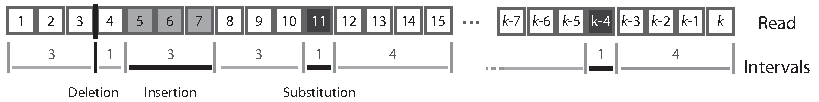
\includegraphics[scale=0.88]{sketch_seeding.pdf}
\caption{\textbf{Read as sequence of error symbols}. Reads consist of
correct nucleotides (white boxes), substitutions (black boxes), deletions
(vertical bars) and insertions (grey boxes).}
\label{fig:sketchseed}
\end{figure}

A read can be partitioned uniquely into maximal sequences of identical
symbols called ``intervals''. Intervals of correct nucleotides will have a
particular importance, so we introduce the somewhat simpler term
``error-free interval''.

\begin{definition}
\label{def:error-free-interval}
An \textbf{error-free interval} is a sequence of correct nucleotides that
cannot be extended left or right.
\end{definition}

Instead of sequences of symbols, reads can be seen as sequences of either
error-free intervals or error symbols (see
figure~\ref{fig:sketchseed_interval}). We will use this construction
throughout section~\ref{sec:seeding}. It will allow us to control the size
of the largest error-free interval (see below).

\begin{figure}[h]
\centering
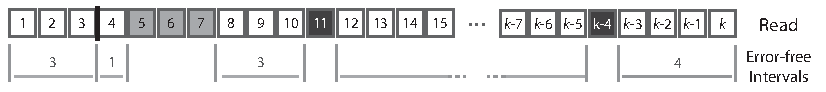
\includegraphics[scale=0.88]{sketch_seeding_error_free_intervals.pdf}
\caption{\textbf{Read as sequence of error-free intervals or error
symbols}.
Consecutive correct nucleotides can be lumped together in error-free
intervals. There is a unique representation of a read as a sequence of
either error-free inetervals or error symbols. The error-free intervals
are highlighted in this example, together with their size.}
\label{fig:sketchseed_interval}
\end{figure}

These formal definitions will allow us to specify the weighted generating
functions of the reads of interest and then approximate their probability
of occurrence using the results of section~\ref{sec:anal}.


\subsection{Exact seeds}

After sequencing, one of the most common operations is to map the
reads in a reference genome, \textit{i.e.} find the identity of the
fragment that was sequenced from a list of candidates. The exact search
problem can be solved efficiently, provided the right indexing data
structures are available, but sequencing errors make the task more
difficult. 

In most mapping algorithms, the search starts by looking for perfect
matches between a fragment of the read and a sequence from the genome.
This match is called a ``seed'', and it allows to quickly eliminate most
of the search space in order to focus on a few promising candidate
sequences.

This strategy greatly accelerates the mapping process, but it is not
failsafe. Seeds are useful only if they are error-free; otherwise they
will either match nothing, or match the wrong sequence. This means that
error-free intervals hold the key to the problem. If there exists a long
enough error-free interval, it may be used as a seed to find the identity
of the read. Here we will use a definition of ``seed'' that correspondso
to this intuition.

\begin{definition}
\label{def:seed}
An \textbf{exact $\gamma$-seed} is an error-free interval of size at least
$\gamma$.
\end{definition}

\begin{remark}
In what follows, we will often refer to an ``exact $\gamma$-seed'' as a
``seed'' when the concrete value of $\gamma$ is either clear from the
context or irrelevant.
\end{remark}

The main goal of section~\ref{sec:seeding} is to develop models to
estimate the probability that a read contains an exact  $\gamma$-seed. Our
strategy is to construct the weighted generating functions of reads that
\emph{do not} contain any exact $\gamma$-seed. For this, we will decompose
such reads as sequences of either error symbols or error-free intervals
of size less than $\gamma$. We will obtain their weighted generating
functions from proposition~\ref{th:HBT} and use proposition~\ref{th:ass}
to approximate their probability of occurrence.

We will find the weighted generating function of all the reads $R(z)$, and
then the weighted generating function of reads without exact
$\gamma$-seeds $S_\gamma(z)$. The probability that a read of size $k$ has
no exact $\gamma$-seed will then be equal to the total weight of reads of
size $k$ without seed, divided by the total weight of reads of size $k$,
\textit{i.e.}

\begin{equation}
\label{eq:THEratio}
\frac{[z^k]S_\gamma(z)}{[z^k]R(z)}.
\end{equation}

To introduce the concepts progressively, we will first describe simplified
models where some types of errors are disallowed, and gradually
increase the complexity towards the model with all error types.





%%%%%%%%%%%%%%%%%% Substitutions only %%%%%%%%%%%%%%%%%%%

\subsection{Substitutions only}
\label{sec:substitutions}

In the simplest model, we assume that errors can be only substitutions,
and that they occur with the same probability $p$ for every nucleotide. We
will refer to this model as the ``uniform substitutions error model''. Due
to its simplicity, we will be able to go at greater depth and obtain more
advanced results with this model (especially in the later sections).
Importantly, the model is not overly simple and it has some real practical
applications. For instance, it describes reasonably well the error model
of the Illumina platforms (where $p$ is around $0.01$).

We will first use proposition~\ref{th:HBT} to obtain the weighted
generating function $R(z)$ of all reads under this error model, from which
we are going to deduce the weighted generating function $S_\gamma(z)$ of
reads without exact $\gamma$-seeds. We will then use
proposition~\ref{th:ass} to derive an approximation formula for the
probability that a read does not contain exact $\gamma$-seeds.

Under the uniform substitutions model, reads are sequences of either
substitutions or error-free intervals. They can be thought of as a walk on
the graph shown in figure~\ref{fig:subonly}. The symbol $\Delta_0$ stands
for error-free intervals and the symbol $S$ stands for single
substitutions. $F(z)$ and $pz$ indicate the weighted generating functions
of error-free intervals and substitutions, respectively. The fact that an
error-free interval cannot follow another error-free interval is a
consequence of the definition: two consecutive intervals must be merged
into a larger interval.

\begin{remark}
In all the error models described in section~\ref{sec:seeding}, the
error-free intervals cannot have size $0$. The reason is that a read must
correspond to exactly one path in the transfer graph and that sequences of
combinatorial classes containing the empty object $\varepsilon$ are not
uniquely defined (see remark~\ref{rem:no_seq_epsilon}).
\end{remark}

\begin{figure}[h]
\centering
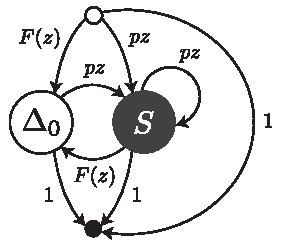
\includegraphics[scale=0.9]{substitutions_only.pdf}
\caption{\textbf{Transfer graph of reads with uniform substitutions}.
Reads are viewed as sequences of error-free intervals (symbol
$\Delta_0$) or substitutions (symbol $S$). $F(z)$ and $pz$ are the
weighted generating functions of error-free intervals and individual
substitutions, respectively.}
\label{fig:subonly}
\end{figure}

A substitution is a single nucleotide and thus has size $1$. Because
substitutions have probability $p$, their weighted generating function is
$pz$. Conversely, the weighted generating function of correct nucleotides
is $qz$. Error-free intervals are non-empty sequences of correct
nucleotides, so by proposition~\ref{th:sequences2} their weighted
generating function is

\begin{equation}
\label{eq:Fsub}
F(z) = qz + (qz)^2 + (qz)^3 + \ldots = \frac{qz}{1-qz}.
\end{equation}

The transfer matrix associated with the body of the transfer graph shown
in figure~\ref{fig:subonly} is

\begin{equation*}
M(z) = 
\begin{blockarray}{ccc}
       & \smDELz & \smS \\
\begin{block}{c[cc]}
\smDELz & 0    & pz \\
\smS    & F(z) & pz \\
\end{block}
\end{blockarray}.
\end{equation*}


A read can start with an error-free interval or with a substitution, so
the head vector $H(z)$ is equal to $(F(z), pz)^\top$. Similarly, a read
can end with an error free interval or with a substitution, so the tail
vector $T(z)$ is equal to $(1,1)^\top$. Here $\psi(z) = 1$, as the only
read excluded by our definition is the empty sequence $\varepsilon$.
Applying proposition~\ref{th:HBT}, the weighted generating function of
reads is $R(z) = \psi(z) + (F(z), pz)^\top \cdot (I-M(z))^{-1} \cdot
T(z)$, or

\begin{equation*}
R(z) = 1 + [F(z) \; pz] \cdot
\frac{1}{\lambda(z)}
\begin{bmatrix}
1-pz & pz   \\
F(z) & 1
\end{bmatrix}
\cdot \begin{bmatrix}1 \\ 1\end{bmatrix},
\end{equation*}
where $\lambda(z) = 1-pz(1+F(z))$ is the determinant of $I-M(z)$.
Finishing the computations, we obtain

\begin{equation}
\label{eq:Rsub}
R(z) = \frac{1+F(z)}{1-pz(1+F(z))} = \frac{1}{1-z}.
\end{equation}

Since $1/(1-z) = 1+z+z^2 + \ldots$, this means that for any $k \geq 0$,
the total weight of reads of size $k$ is equal to $1$. As a consequence,
ratio (\ref{eq:THEratio}) reduces to $[z^k]S_\gamma(z)$.

To find the weighted generating function of reads without any exact
$\gamma$-seeds, we need to limit error-free intervals to a maximum size of
$\gamma-1$. To do this, we can replace $F(z)$ in (\ref{eq:Rsub}) by its
truncation $F_\gamma(z) = qz + (qz)^2 + \ldots + (qz)^{\gamma-1}$. We
obtain

\begin{equation}
\label{eq:Sp}
S_\gamma(z) = \frac{1+F_\gamma(z)}{1-pz\big( 1+F_\gamma(z) \big)} =
\frac{1+qz + \ldots + (qz)^{\gamma-1}}{1-pz \big(1+qz + \ldots +
(qz)^{\gamma-1} \big)}.
\end{equation}

\begin{remark}
Viewing reads as sequences of either error-free intervals or substitutions
was important to obtain the weighted generating function of reads without
seeds. It allowed us to just replace $F(z)$ by $F_\gamma(z)$ to find the
expression immediately.
\end{remark}

The task is now to extract the coefficient of $z^k$ in $S_\gamma(z)$. As
explained in section~\ref{sec:asest}, we look for an asymptotic estimate
using proposition~\ref{th:ass}. For this, we need to find the
singularities of $S_\gamma(z)$.

It is interesting to look in detail into the problem of finding the
singularities of $S_\gamma(z)$. To higlight some general features of the
problem, we start with a concrete case. The left panel of
Figure~\ref{fig:plotQ} shows the values of the denominator of
$S_\gamma(z)$ with $p=0.1$ and $\gamma=17$. $S_{17}$ has one real root
greater than $1$.  The remaining singularities of $S_{17}$ are complex and
they seem to be evenly spaced on the same circle, as can be seen on the
right panel of Figure~\ref{fig:plotQ}.  This is only a visual impression.
In fact the singularities are not exactly on the same circle and their
rotation angles are not exactly regular.

\begin{figure}[h]
\centering
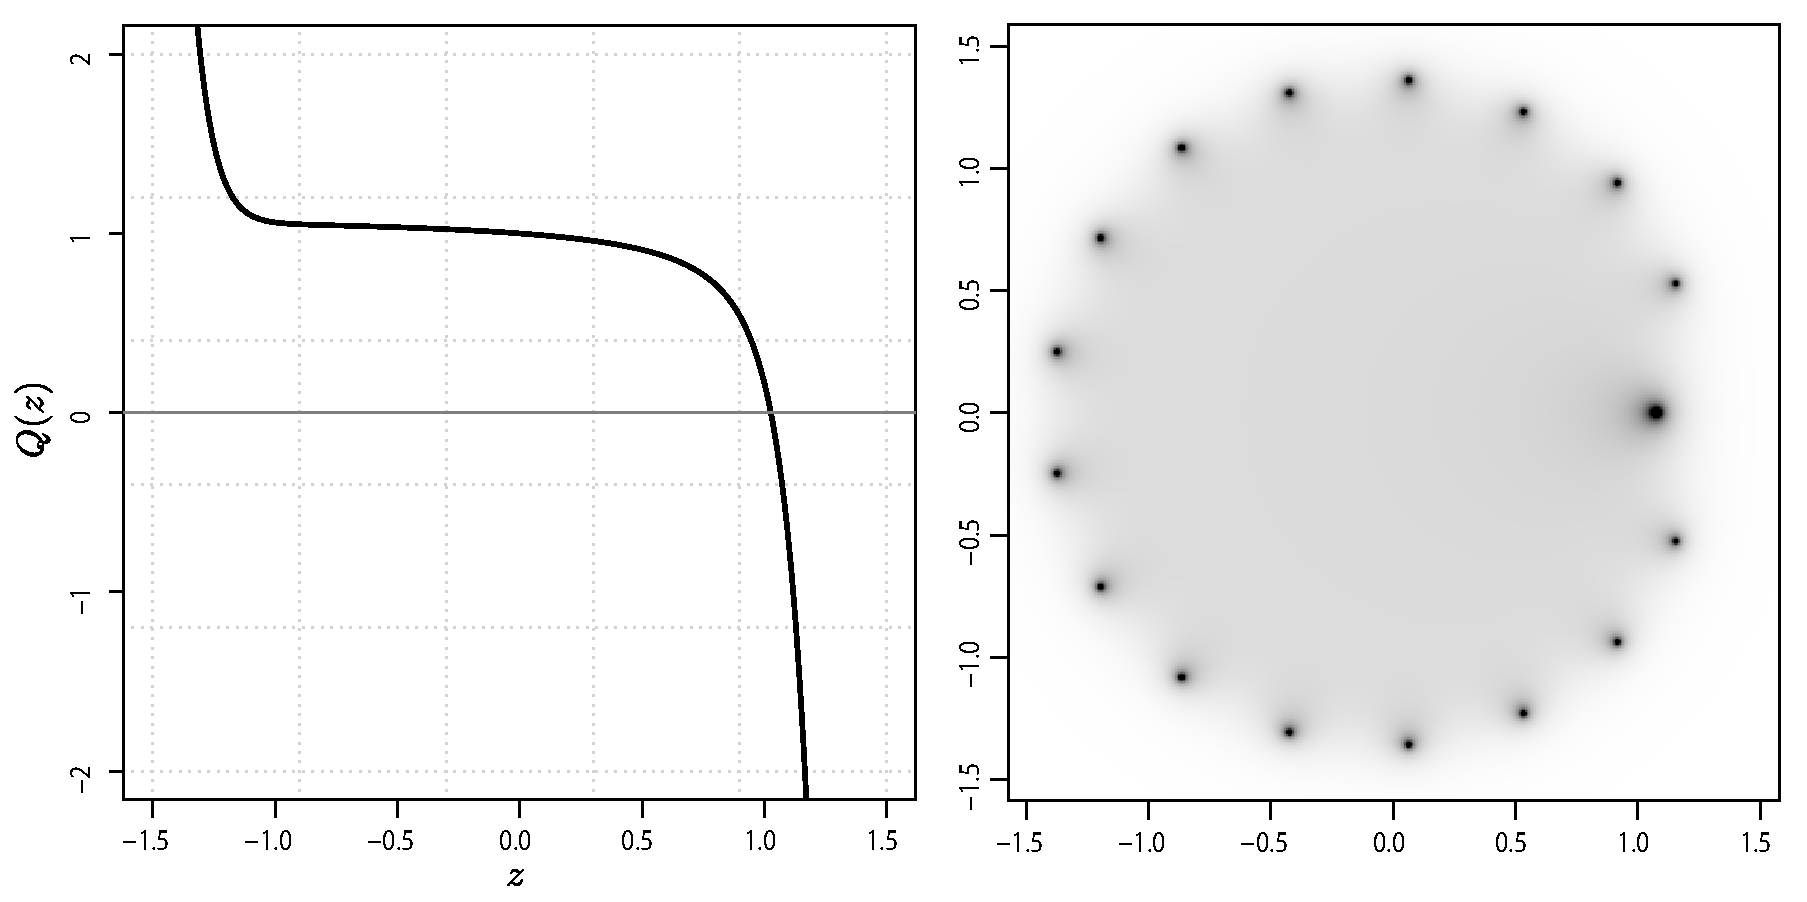
\includegraphics[scale=0.4]{singularityS.pdf}
\caption{\textbf{Singularities of $S_{17}$}. $Q(z)$ denotes the
denominator of $S_{17}(z)$ from expression (\ref{eq:Sp}) with $p=0.1$ and
$\gamma=17$. \textit{Left}: The value of $Q(z)$ is represented for $z$
real by the bold line. \textit{Right}: The value of $|1/Q(z)|$ is
represented for $z$ complex by the heat map on the complex plane. Darker
pixels correspond to higher values. Sixteen singularities of $S_{17}$ lie
close to a circle. The remaining seventeenth is the one shown on the left
panel. It is the dominant singularity because it is the closest to the
origin.}
\label{fig:plotQ}
\end{figure}

It is ``fortunate'' that the dominant root of $S_{17}$ is a real number
because we can use efficient numerical methods to approximate it
(\textit{e.g.} bisection or the Newton-Raphson method). The following
proposition shows that this is no accident: the dominant singularity of
$S_\gamma$ is always a real positive number greater than $1$.

\begin{proposition}
\label{th:roots}
$S_\gamma$ as expressed in (\ref{eq:Sp}) has exactly one positive real
singularity. This is the dominant singularity and it is greater than $1$.
\end{proposition}

\begin{proof}
Write $S_\gamma(z) = P(z)/Q(z)$ and search the roots of the denominator
$Q(z) = 1-pz(1+qz+\ldots+(qz)^{\gamma-1})$.
First, we show that $Q$ has exactly one positive real root greater than
$1$. For real $z > 0$, $pz$ and $1+qz+\ldots+(qz)^{\gamma-1}$ are strictly
increasing, so $Q(z)$ is strictly decreasing. Since $Q(1) = q^d > 0$ there
is no root in the interval $(0,1)$ and since $\lim_{z\rightarrow \infty}
Q(z) = -\infty$, $Q$ vanishes for a real number greater than $1$.

Second, we show that this is the root with smallest \textit{modulus}.
Express the complex roots of $Q$ as $Re^{i\theta}$. They satisfy the
equation

\begin{equation*}
1-pRe^{i\theta}\frac{1-q^\gamma R^\gamma
e^{i\gamma\theta}}{1-qRe^{i\theta}} = 0,
Re^{i\theta} \neq \frac{1}{q}.
\end{equation*}

Multiplying through by $1-qRe^{i\theta}$, we obtain an equation of which
we separate the real and the imaginary parts to obtain

\begin{equation*}
\left\{
\begin{array}{ll}
pR \cos (\theta) -1 = pq^\gamma R^{\gamma+1}
\cos \big( (\gamma+1) \theta \big) \\
pR \sin (\theta) = pq^\gamma R^{\gamma+1}
\sin \big( (\gamma+1) \theta \big)
\end{array}
\right. Re^{i\theta} \neq \frac{1}{q}.
\end{equation*}

Squaring and summing, we obtain the following equation

\begin{equation}
\label{eq:Reitheta}
p^2R^2 = (pq^\gamma R^{\gamma+1})^2 + 2pR \cos(\theta) -1.
\end{equation}

Considering this an equation of $R > 0$, the solution is minimal when
$2pR\cos(\theta)$ is maximal, \textit{i.e.} when $\theta = 0$. In other
words, if there is a positive real root, its \textit{modulus} is the
minimum among the roots. We have seen above that there exsists exactly
one, so it is the dominant singularity of $S_\gamma$.
\end{proof}

We now have all the tools to approximate the coefficients of $S_\gamma(z)$
using proposition~\ref{th:ass} and obtain the approximate probability that
a read contains no seed.

\begin{proposition}
\label{th:p}
The probability that a read of size $k$ has no seed under the uniform
substitutions model is asymptotically equivalent to

\begin{equation*}
\frac{C}{z_1^{k+1}},
\end{equation*}
where $z_1$ is the only real positive root of
$1-pz(1+qz+\ldots+(qz)^{\gamma-1})$, and where

\begin{equation}
\label{eq:Cp}
C =\frac{(1-qz_1)^2}{p^2 z_1
\big( 1-(\gamma+1-\gamma qz_1)(qz_1)^\gamma \big)}.
\end{equation}
\end{proposition}

\begin{proof}
Apply propositions~\ref{th:ass} to $S_\gamma(z)$ and then
proposition~\ref{th:roots}, together with the fact that for any
singularity $z$ of $S_\gamma$ we have $1+qz+\ldots+(qz)^{\gamma-1} =
1/pz$.
\end{proof}

We now illustrate proposition~\ref{th:p} with a concrete example
explaining how the calculations are done in practice.

\begin{example}
\label{ex:num1}
Let us approximate the probability that a read of size $k=100$ has no seed
for $\gamma=17$ and for a substitution rate $p=0.1$. To find the dominant
singularity of $S_{17}$, we need to solve
$1-0.1z\times(1+0.9z+\ldots+(0.9z)^{16}) = 0$. We rewrite the equation as
$1 - 0.1z\times(1-(0.9 z)^{17})/(1-0.9z) = 0$ and use bisection to solve
it numerically, yielding $z_1 \approx 1.0268856$. Substituting this value
in (\ref{eq:Cp}) yields $C \approx 1.396145$, so the probability that a
read contains no seed is approximately $1.396145 / 1.0268856^{101} \approx
0.095763$. For comparison, a 99\% confidence interval obtained by
performing 10 billion random simulations is $0.09575-0.09577$.
% The magic number is 957598614 out of 10 billion.
The computational cost of the analytic combinatorics approach is
infinitesimal compared to the random simulations, and the precision
is much higher for $k=100$.
\end{example}

\begin{figure}[h]
\centering
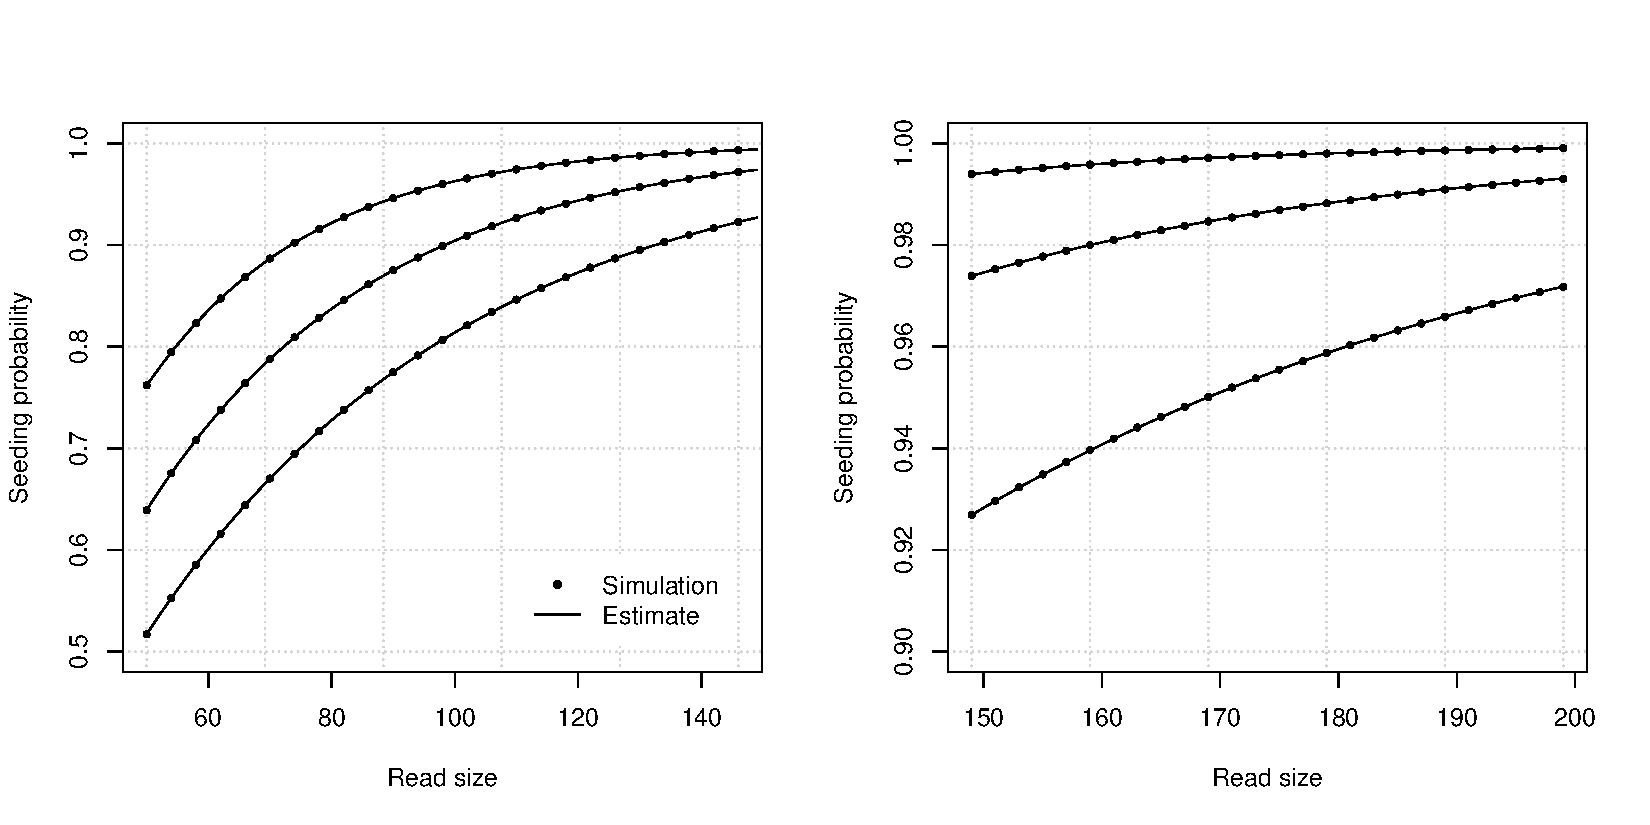
\includegraphics[scale=0.445]{simulp.pdf}
\caption{\textbf{Example estimates for substitutions only}. The analytic
combinatorics estimates of proposition~\ref{th:p} are benchmarked against
random simulations. Shown on both panels are the probablities that a read
of given size contains a seed, either estimated by 10,000,000 random
simulations (dots), or by the method described above (lines). The curves
are drawn for $\gamma=17$ and $p=0.08$, $p=0.10$ or $p=0.12$ (from top to
bottom).}
\label{fig:simulp}
\end{figure}

Overall, the analytic combinatorics estimates are close to the exact
values. Figure~\ref{fig:simulp} illustrates the precision of the estimates
for different values of the error rate $p$ and of the read size $k$.



%%%%%%%%%%%%%%%%% Subsitutions and deletions %%%%%%%%%%%%%%%%%%

\subsection{Substitutions and deletions}
\label{sec:deletions}

To not jump too fast into the difficulties, we will now describe a
semi-realistic model where errors can be deletions or susbtitutions, but
not insertions. As in the case of uniform substitutions, we assume that
every nucletoide call is false with a probability $p$ and true with a
probability $1-p=q$. Here, we also assume that the ``space''  between
consecutive nucleotides can contain a deletion with probability $\delta$.

A deletion may be adjacent to a substitution, or lie in between two
correct nucleotides. In the first case, the deletion does not interrupt
any error-free interval so it does not change the probability that the
read contains a seed. For this reason, we ignore deletions next to
substitutions. More precisely, we assume that they can occur, but whether
they do has no importance for the problem.

Under this error model, a read can be thought of as a walk on the graph
shown in figure~\ref{fig:deletions}. The graph is almost the same as the
one shown figure~\ref{fig:subonly}; the only difference is the edge
labelled $\delta F(z)$ from $\Delta_0$ to $\Delta_0$. This edge represents
the fact that under this error model, an error-free interval can follow
another one if a deletion with weighted generating function $\delta$ is
present in between (as illustrated for instance in
figure~\ref{fig:sketchseed_interval}).

\begin{figure}[h]
\centering
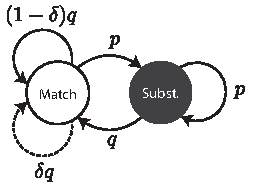
\includegraphics[scale=0.9]{deletions.pdf}
\caption{\textbf{Transfer graph of reads with uniform substitutions and
deletions}. Reads are viewed as sequences of error-free intervals (symbol
$\Delta_0$) or substitutions (symbol $S$). An error-free interval can
follow another one if a deletion is present in between. $F(z)$ and $pz$
are the weighted generating functions of error-free intervals and
individual substitutions, respectively. $\delta F(z)$ is the weighted
generating function of a deletion followed by an error-free interval.}
\label{fig:deletions}
\end{figure}

The weighted generating function of error-free intervals $F(z)$ has a
different expression from that of section~\ref{sec:substitutions}. When
the size of an error-free interval is $1$, the weighted generating
function is just $qz$. For a size $k > 1$, there are $k-1$ ``spaces''
between the nucleotides, so the weighted generating function is
$(1-\delta)^{k-1}(qz)^k$. Summing for all the possible sizes, we obtain
the weighted generating function of error-free intervals as

\begin{equation}
\label{eq:Fdel}
F(z) = qz + (1-\delta)(qz)^2 + (1-\delta)^2(qz)^3 + \ldots =
\frac{qz}{1-(1-\delta)qz}.
\end{equation}

The transfer matrix associated with the body of the transfer graph shown
in figure~\ref{fig:deletions} is

\begin{equation*}
M(z) = 
\begin{blockarray}{ccc}
       & \smDELz & \smS \\
\begin{block}{c[cc]}
\smDELz & \delta F(z) & pz \\
\smS    &        F(z) & pz \\
\end{block}
\end{blockarray}.
\end{equation*}

The head and tail vectors are the same as in
section~\ref{sec:substitutions}, \textit{i.e}
$H(z) = (F(z), pz)^\top$, $T(z) = (1,1)^\top$ and $\psi(z) = 1$.
Applying proposition~\ref{th:HBT} yields

\begin{equation*}
R(z) = (I-M(z))^{-1} =
1 + [F(z) \; pz] \cdot \frac{1}{\lambda(z)}
\begin{bmatrix}
1-pz  & pz              \\
F(z) & 1 -\delta F(z)
\end{bmatrix}
\cdot \begin{bmatrix}1 \\ 1\end{bmatrix},
\end{equation*}
where $\lambda(z) = 1-pz-(pz(1-\delta)+\delta)F(z)$ is the determinant of
$I-M(z)$. Finishing the computations we obtain

\begin{equation}
\label{eq:Rdel}
R(z) = \frac{1+(1-\delta)F(z)} {1-pz - \big(pz(1-\delta) + \delta\big)F(z)}
= \frac{1}{1-z}.
\end{equation}

As in section~\ref{sec:substitutions} the result is $1/(1-z) = 1+z +z^2 +
\ldots$, which means that the total weight of reads of size $k$ is equal
to $1$ for every $k \geq 0$. This means that ratio (\ref{eq:THEratio})
reduces one again to $[z^k]S_\gamma(z)$.

To find the weighted generating function of reads without any exact
$\gamma$-seeds, we need to bound the size of error-free intervals to a
maximum of $\gamma-1$, \textit{i.e.} to replace $F(z)$ by its truncation
$F_\gamma(z) = qz + (1-\delta)(qz)^2 + \ldots +
(1-\delta)^{\gamma-2}(qz)^{\gamma-1}$. With this definition, the weighted
generating function of seedless reads is

\begin{equation}
\label{eq:Sdel}
S_\gamma(z) = \frac{1+(1-\delta)F_\gamma(z)}
  {1-pz - \big(pz(1-\delta) + \delta\big)F_\gamma(z)}.
\end{equation}

Applying proposition~\ref{th:ass} to this expression, we obtain the
following approximation formula.

\begin{proposition}
\label{th:pd}
The probability that a read of size $k$ has no seed under the model of
uniform substitutions and deletions is asymptotically
equivalent to

\begin{equation*}
\frac{C}{z_1^{k+1}},
\end{equation*}
where $z_1$ is the only real positive root of the denominator of
$S_\gamma(z)$, \textit{i.e.} the root of $1-pz - \big(pz(1-\delta) +
\delta\big)\big(qz+(1-\delta)(qz)^2 + \ldots +
(1-\delta)^{\gamma-2}(qz)^{\gamma-1}\big)$, and

\begin{equation}
\label{eq:Cpd}
\begin{split}
C &=
\frac{ z_1 \big(1-(1-\delta)(1-p)z_1\big)^2 }
{ \big((p+q\delta)z_1  -c_1(1-\delta)^{\gamma-1}(qz_1)^\gamma \big)
\big(\delta+(1-\delta)pz_1\big) }\text{, where} \\
c_1 &= \gamma\delta -(1-\delta)\big((\gamma-1)\delta
-p((\gamma-1)\delta+\gamma+1)\big)z_1
- \gamma(1-\delta)^2pqz_1^2.
\end{split}
\end{equation}
\end{proposition}

We illustrate proposition~\ref{th:pd} with a concrete example explaining
how the calculations are done in practice.

\begin{example}
\label{ex:num2}
Let us approximate the probablity that a read of size $k = 100$ has
no seed for $\gamma=17$, $p = 0.05$ and $\delta = 0.15$. To find
the dominant singularity of $S_{17}$ we solve $1-0.05z -
\big(0.0425z + 0.15\big) \big(0.95z+0.85(0.95z)^2 + \ldots +
0.85^{15}(0.95z)^{16}\big) = 0$. We write it as $1-0.05z - \big(0.0425z +
0.15) (0.95z-0.85^{16}(0.95z)^{17}) / (1-0.8075z) = 0$ and use bisection,
yielding $z_1 \approx 1.006705$. Now substituting the
obtained value in (\ref{eq:Cpd}) gives $C \approx 1.096177$, so the
probability that a read contains no seed is approximately $1.096177 /
1.006705^{101} \approx 0.558141$. For comparison, a 99\% confidence
interval obtained by performing 10 billion random simulations is
$0.55813-0.55816$.
% The magic number is 5581417733 out of 10 billion.
\end{example}

\begin{figure}[h]
\centering
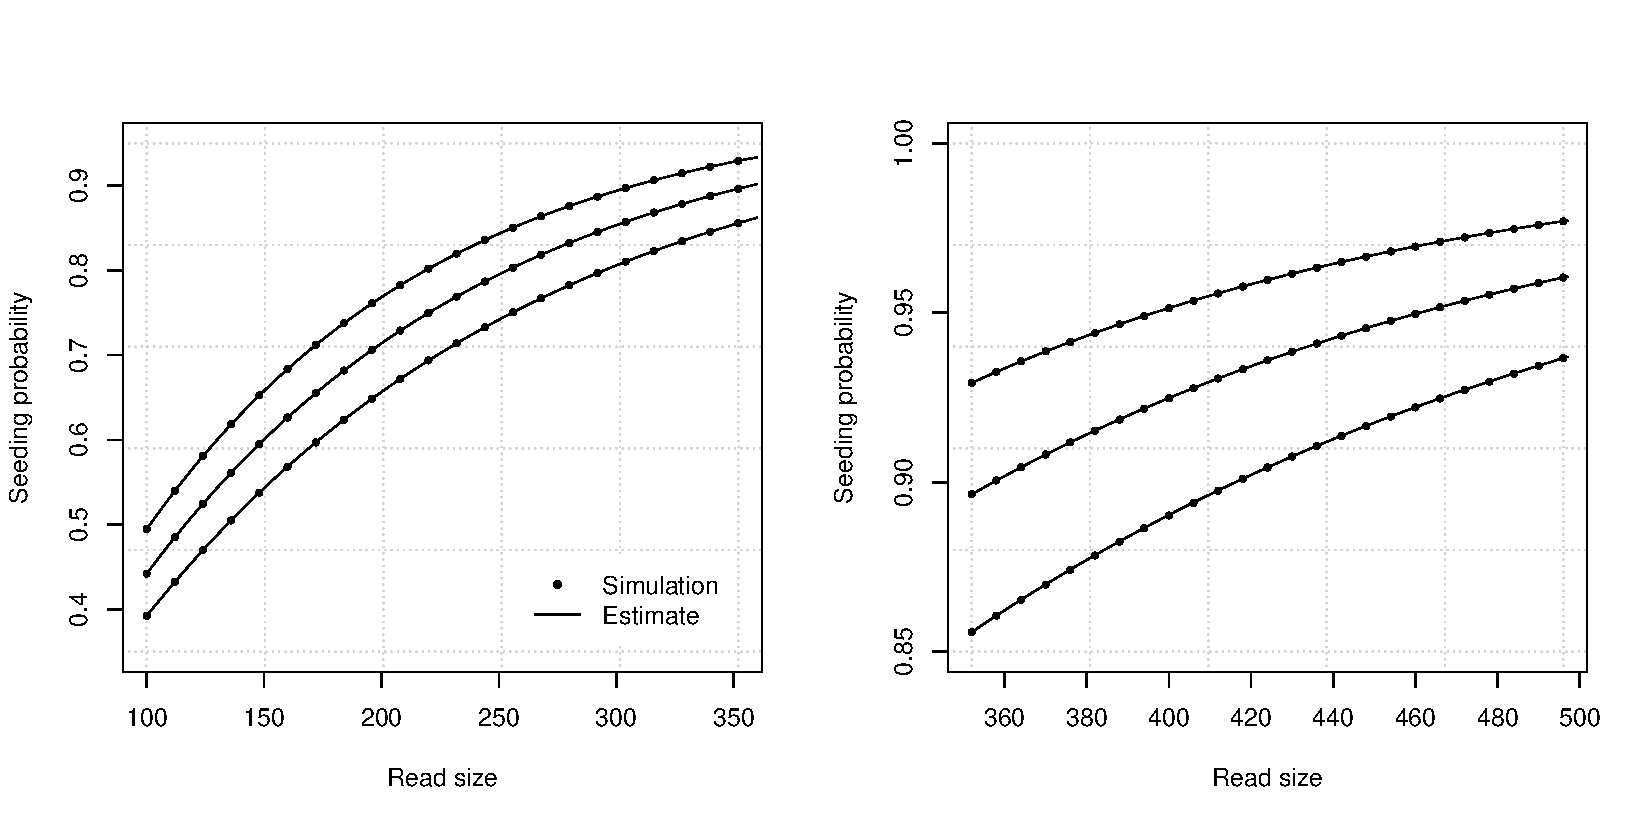
\includegraphics[scale=0.445]{simulpdel.pdf}
\caption{\textbf{Example estimates for substitutions and deletions}. The
analytic combinatorics estimates of proposition~\ref{th:pd} are
benchmarked against random simulations. Shown on both panels are the
probablities that a read of given size contains a seed, either estimated
by 10,000,000 random simulations (dots), or by proposition~\ref{th:pd}
(lines). The curves are drawn for $\gamma=17$, $p=0.05$ and $\delta=0.14$,
$\delta=0.15$ or $\delta=0.16$ (from top to bottom).}
\label{fig:simulpdel}
\end{figure}

Once again, the analytic combinatorics estimates are close to the exact
values. Figure~\ref{fig:simulpdel} illustrates the precision of the
estimates for different values of the deletion rate $\delta$ and of the
read size $k$.



%%%%%%%%%%% Subsitutions, deletions and insertions %%%%%%%%%%%%

\subsection{Substitutions, deletions and insertions}
\label{sec:insertions}

Here we consider the model that we will refer to as ``full error model''
because all types of errors are allowed. Introducing insertions brings two
additional difficulties. The first is that a substitution is
indistinguishable from an insertion followed by a deletion (or a deletion
followed by an insertion). By convention, we will count all these cases as
substitutions. As a consequence, a deletion can never be found next to an
insertion. The second difficulty is that insertions usually come in
bursts. This is also the case of deletions, but we could neglect it
because this does not affect the size of the interval (all deletions have
size $0$). 

To model insertion bursts, we need to assign a probability $r$ to the
first insertion, and a probability $\tilde{r} > r$ to all subsequent
insertions of the burst. We will still denote the probability of a
substitution $p$ and that of a correct call $q$, but here $p+q+r=1$. We
will also assume that an insertion burst stops with probability
$1-\tilde{r}$ at each position of the burst.

Under this error model, reads can be thought of as a walk on the graph
shown in figure~\ref{fig:insertions}. The symbols $\Delta_0$, $S$ and $I$
stand for error-free intervals, single substitutions and single
insertions, respectively. The body of the graph is represently separately
from the head and tail vertices to avoid overloading the figure.

The terms $F(z)$, $pz$ and $\delta F(z)$ are the same as in
section~\ref{sec:deletions}. The terms $rz$ and $\tilde{r}z$ are the
weighted generating functions of the first inserted nucleotide and of all
subsequent nucleotides of the insertion burst, respectively. The burst can
terminate with an error-free interval or with a substitution, with
respective weighted generating functions $(1-\tilde{r})F(z)$ and
$(1-\tilde{r})pz$.


\begin{figure}[h]
\centering
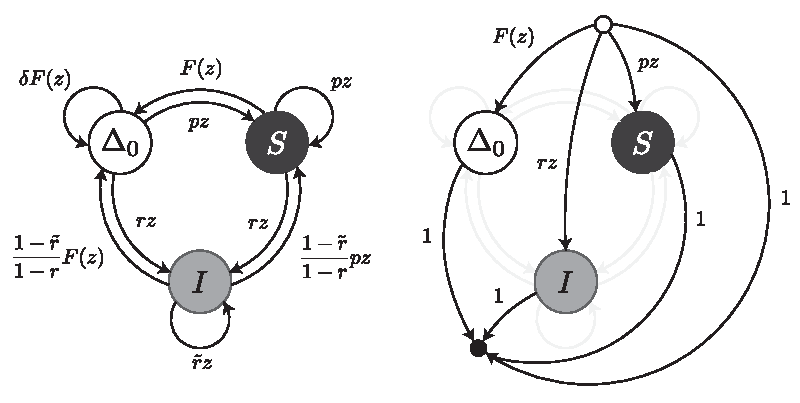
\includegraphics[scale=0.9]{insertions.pdf}
\caption{\textbf{Transfer graph of reads with full error model}. Reads are
viewed as sequences of error-free intervals (symbol $\Delta_0$),
substitutions (symbol $S$) or insertions (symbol $I$). To not overload the
figure, the body of the transfer graph is shown on the left, and the head
and tail edges are shown on the right. $F(z)$ and $pz$ are the weighted
generating functions of error-free intervals and individual substitutions,
respectively. $\delta F(z)$ is the weighted generating function of a
deletion followed by an error-free interval. $rz$ and $\tilde{r}z$ are the
weighted generating functions of the first and all subsequent insertions
of a burst, respectively. $(1-\tilde{r})F(z)$ is the weighted generating
function of an error-free interval following an insertion and
$(1-\tilde{r})pz$ is the weighted generating function of a substitutition
following an insertion.}
\label{fig:insertions}
\end{figure}


The expression of the weighted generating function of error-free intervals
$F(z)$ is the same as insection~\ref{sec:deletions}, namely

\begin{equation*}
F(z) = qz + (1-\delta)(qz)^2 + (1-\delta)^2(qz)^3 + \ldots =
\frac{qz}{1-(1-\delta)qz}.
\end{equation*}

The transfer matrix associated with the body of the transfer graph shown
in figure~\ref{fig:insertions} is

\begin{equation*}
M(z) = 
\begin{blockarray}{cccc}
       & \smDELz & \smS & \smI \\
\begin{block}{c[ccc]}
\smDELz & \; \delta F(z) & pz & rz \; \\
\smS    & \;        F(z) & pz & rz \; \\
\smI    & \; (1-\tilde{r})F(z)
           & (1-\tilde{r})pz & \tilde{r}z \; \\
\end{block}
\end{blockarray}.
\end{equation*}

Here the head vector $H(z)$ is equal to $(F(z), pz, rz)^\top$, the tail
vector $T(z)$ is equal to $(1,1,1)^\top$, and $\psi(z) = 1$. The
expression of $(I-M(z))^{-1}$ is omitted because it is cumbersome, but
according to proposition~\ref{th:HBT} all we need is the value of
$\psi(z)+H(z)^\top \cdot (I-M(z))^{-1} \cdot T(z)$. Finishing the
calculations, we find

\begin{equation}
\label{eq:Rindel}
R(z) = \frac{\big( 1-(\tilde{r}-r)z \big)
\left(1+(1-\delta)F(z) \right)}{1-a(z)-b(z)F(z)}
= \frac{1}{1-z},
\end{equation}
where

\begin{equation}
\begin{gathered}
\label{eq:a+b}
%a(z) = r-\big((p+\tilde{r})r-\tilde{r}-p\big)z
%- p(\tilde{r}-r)z^2\text{, and} \\
%b(z) = \delta(1-r) - \big((\tilde{r}\delta-(1-\delta)p)(1-r)
%-(1-\tilde{r})r\big)z -(1-\delta)p(\tilde{r}-r)z^2.
a(z) = (p+\tilde{r})z + p\big(\tilde{r}-r(1-\tilde{r})\big)z^2 \\
b(z) = \delta + \big(p(1-\delta) - \tilde{r}(\delta+r)+r\big)z
+ p(1-\delta)\big(r-\tilde{r}(1+r)\big)z^2.
\end{gathered}
\end{equation}


Again, the terms cancel out and we obtain the simple expression $1/(1-z) =
1+z+z^2 + \ldots$ where all the coefficients are equal to $1$. This means
that once again, ratio (\ref{eq:THEratio}) reduces to $[z^k]S_\gamma(z)$.
To find the weighted generating function of reads without an exact
$\gamma$-seeds, we replace $F(z)$ in expression (\ref{eq:Rindel}) by its
truncated version

\begin{equation*}
F_\gamma(z) = qz + (1-\delta)(qz)^2 + (1-\delta)^2(qz)^3 + \ldots +
(1-\delta)^{\gamma-2}(qz)^{\gamma-1}.
\end{equation*}

We obtain the following expression, where $a(z)$ and $b(z)$ are defined in
(\ref{eq:a+b})

\begin{equation}
\label{eq:Sindel}
S_\gamma(z) =
\frac{\big( 1-(\tilde{r}-r)z \big) \left(1+(1-\delta)F_\gamma(z)
\right)}{1-a(z)-b(z)F_\gamma(z)}.
\end{equation}


\begin{remark}
\label{rem:russian_dolls}
Note that when $r = \tilde{r} = 0$, $a(z) = pz$ and $b(z) = pz(1-\delta) +
\delta$, so expression (\ref{eq:Sindel}) becomes

\begin{equation*}
S_\gamma(z) = \frac{1 + (1-\delta)F_\gamma(z)}
{1-pz-(pz(1-\delta)+\delta))F_\gamma(z)}.
\end{equation*}

This is expression (\ref{eq:Sdel}), \textit{i.e.} the model described in
section~\ref{sec:deletions}. When we also have $\delta = 0$, this
expression further simplifies to

\begin{equation*}
S_\gamma(z) = \frac{1 + F_\gamma(z)}{1-pz(1 + F_\gamma(z))}.
\end{equation*}

This is expression (\ref{eq:Sp}), \textit{i.e.} the model described in
section~\ref{sec:substitutions}. In other words, the error models
described previously are special cases of the full error model.
\end{remark}

As in the previous sections, we can use proposition~\ref{th:ass} to obtain
asymptotic approximations for the probability that the reads contain no
seed.


\begin{proposition}
\label{th:pins}
The probability that a read of size $k$ has no seed under the full error
model is asymptotically equivalent to

\begin{equation*}
\frac{C}{z_1^{k+1}},
\end{equation*}
where $z_1$ is the only real positive root of the polynomial
$1-a(z)-b(z)F_\gamma(z) = 1-a(z)-b(z)\big(qz+(1-\delta)(qz)^2 + \ldots +
(1-\delta)^{\gamma-2}(qz)^{\gamma-1}\big)$, and $C = c_1 / c_2$, with

\begin{equation*}
c_1 = (1-(\tilde{r}-r)z_1)
   \frac{1-\big((1-\delta)(qz)\big)^\gamma}{1-(1-\delta)qz}
\end{equation*}
and
\begin{equation*}
\begin{split}
c_2 = a'(z_1) &- \left( b'(z_1) +
\frac{(1-\delta)q}{1-(1-\delta)qz}\right)
\frac{qz-(1-\delta)^{\gamma-1}(qz)^\gamma}{1-(1-\delta)qz} \\
&+b(z_1) \frac{q-\gamma(1-\delta)^{\gamma-1}q^\gamma
z^{\gamma-1}}{1-(1-\delta)qz}.
\end{split}
\end{equation*}
\end{proposition}

We illustrate proposition~\ref{th:pins} with a concrete example
explaining how the calculations are done in practice.

\begin{example}
\label{ex:num3}
Let us approximate the probability that a read of size $k=100$ has no seed
for $\gamma=17$, $p=0.05$, $\delta=0.15$, $r=0.05$ and
$\tilde{r}=0.45$. With these values, $a(z) = 0.05 +0.475z -0.02z^2$ and
$b(z) = 0.1425 + 0.00375z-0.017z^2$. We need to solve $0.95-0.475z+0.02z^2
- (0.1425
+0.00375z-0.017z^2)(0.9z+0.85(0.9z)^2+\ldots+0.85^{15}(0.9z)^{16}) = 0$.
We rewrite the equation as $0.95-0.475z+0.02z^2 - (0.1425
+0.00375z-0.017z^2)(0.9z-0.85^{15}(0.9z)^{16})/(1-0.765z) = 0$ and use
bisection to solve it numerically, yielding $z_1 \approx 1.00295617$.
Using proposition~\ref{th:pins}, we obtain $C \approx 1.042504$, so the
probability that a read contains no seed is approximately $1.042504 /
1.00295617^{101} \approx 0.773749$. For comparison, a 99\% confidence
interval obtained by performing 10 billion random simulations is
$0.77373-0.77376$.
% The magic number is 7737489777 out of 10 billion.
\end{example}

Once again, the analytic combinatorics estimates are close to the exact
values. Figure~\ref{fig:simulpins} illustrates the precision of the
estimates for different values of the insertion rate $r$ and of the read
size $k$.

\begin{figure}[h]
\centering
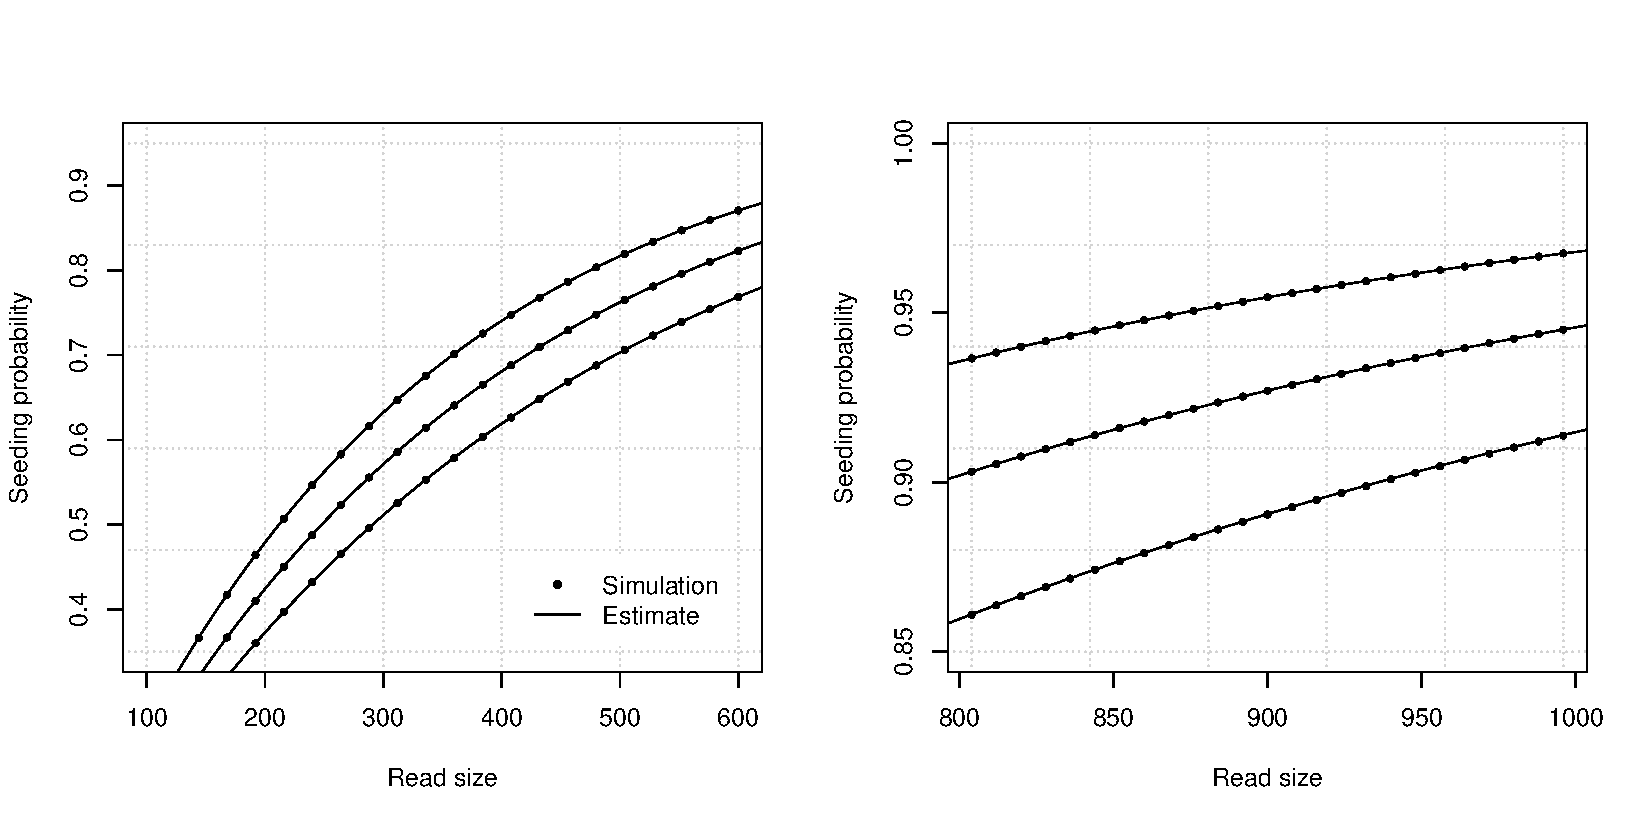
\includegraphics[scale=0.445]{simulpins.pdf}
\caption{\textbf{Example estimates for substitutions, deletions and
insertions}. The analytic combinatorics estimates of
proposition~\ref{th:pins} are benchmarked against random simulations.
Shown on both panels are the probablities that a read of given size
contains a seed, either estimated by 10,000,000 random simulations (dots),
or by the method described above (lines). The curves are drawn for
$\gamma=17$, $p=0.05$, $\delta=0.15$, $\tilde{r} = 0.45$ and $r=0.04$,
$r=0.05$ or $r=0.06$ (from top to bottom).}
\label{fig:simulpins}
\end{figure}




%%%%%%%%%%%%%%%%%%%% Empirical error models %%%%%%%%%%%%%%%%%%

\subsection{Empirical error models}
\label{subsec:empirical}

In the theory developed so far, we introduced different kinds of errors
because they have different probabilities and different sizes, but the
nature of the error is irrelevant. To know whether the read contains a
perfect seed, only their distribution matters.

An important consequence is that we can develop custom error models based
on empirical estimates of the error distribution. This option is not only
valid for modeling sequencing errors, but also for modeling mutations
occurring through biological processes.

We introduce error-only intervals, which will encapsulate the available
information about the size of error patches. Treating deletions separately
will allow us to simplify the exposition, so we will consider that
error-only intervals are always be non-empty.

\begin{definition}
\label{def:error-interval}
An \textbf{error-only interval} is a non-empty sequence of errors that
cannot be extended left or right.
\end{definition}

We assume that every nucleotide has a constant probability $q$ of being
correct. With probability $p = 1-q$, the nucleotide is incorrect and thus
starts an error-only interval. If  $p_k$ is the empirical probability that
the error-only interval has size $k$ for $1 \leq k \leq n$, we can write
the weighted generating function of error intervals as $pE(z)$, where
$E(z) = p_1z + p_2z^2 + \ldots + p_nz^n$.

The weighted generating function of deletions is denoted $\delta$ for
consistency with the previous sections. As before, we will ignore
deletions adjacent to error-only intervals. Even if they occur, they have
no consequence as they never interrupt a potential seed.

Reads under the empirical error model can be thought of as walks on the
transfer graph shown in figure~\ref{fig:empirical}.
An error-free interval can be followed by an error-only interval, or by
another error-free interval if a deletion is present in between. An
error-only interval can only be followed by an error-free interval.

\begin{figure}[h]
\centering
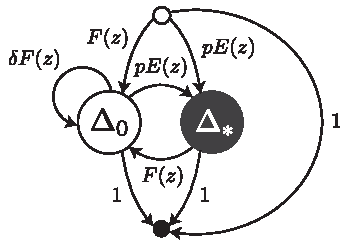
\includegraphics[scale=0.9]{empirical.pdf}
\caption{\textbf{Transfer graph of reads under the empirical error model}.
Reads are viewed as sequences of error-free intervals (symbol $\Delta_0$)
or error-only intervals (symbol $\Delta_*$). An error-free interval can
follow another one if a deletion is present in between. $F(z)$ and $pE(z)$
are the weighted generating functions of error-free intervals and
error-only intervals, respectively. $\delta F(z)$ is the weighted
generating function of a deletion followed by an error-free interval.}
\label{fig:empirical}
\end{figure}

The head and tail vectors are $(F(z), pE(z))^\top$ and $(1,1)$,
respectively; and $\psi(z) = 1$. The transfer matrix associated with the
body of the transfer graph shown in figure~\ref{fig:empirical} is

\begin{equation*}
M(z) = 
\begin{blockarray}{ccc}
       & \smDELz & \smDELs \\
\begin{block}{c[cc]}
\smDELz & \delta F(z)  & p E(z) \\
\smDELs & F(z)         &   0    \\
\end{block}
\end{blockarray}.
\end{equation*}


Computing $\psi(z) + H(z)^\top \cdot (I-M(z))^{-1} \cdot T(z)$ as per
proposition~\ref{th:HBT} yields

\begin{equation*}
1+[F(z) \; pE(z)] \cdot \frac{1}{1-F(z)(\delta+pE(z))} \cdot
\begin{bmatrix}
1    & pE(z) \\
F(z) & 1-\delta F(z)
\end{bmatrix} \cdot
\begin{bmatrix}1 \\ 1\end{bmatrix},
\end{equation*}
which eventually simplifies to

\begin{equation}
\label{eq:Remp0}
R(z) = 
\frac{\big(1+(1-\delta)F(z)\big)\big(1+pE(z)\big)}
   {1-F(z)\big(\delta+pE(z)\big)}.
\end{equation}

As previously, the weighted generating function of error-free intervals is
$F(z) = qz + (1-\delta)(qz)^2 + (1-\delta)^2(qz)^3 + \ldots =
qz/(1-(1-\delta)qz)$. Substituting this value in the equation above, we
obtain

\begin{equation}
\label{eq:Remp}
R(z) = \frac{1+pE(z)}{1-qz\big(1+pE(z)\big)}.
\end{equation}

Epxression (\ref{eq:Remp}) is in general not equal to $1/(1-z)$ because
$E(z)$ is not equal to $z/(1-pz)$. Since the total weight of reads of size
$k$ is not equal to $1$, we cannot simplify ratio (\ref{eq:THEratio}) as
in the previous cases. We will need to include $[z^k]R(z)$ in our
calculations, which we will approximate with proposition~\ref{th:ass}.
This implies that we have to find the root with smallest \textit{modulus}
of the polynomial $1-qz\big(1+\delta+E(z)\big)$.

\begin{remark}
Why $[z^k]R(z) = 1$ for some models but not for others? The combinatorial
``atoms'' can be inhomogeneous, leading to a weight deficit for certain
sequence sizes. For instance, sequences of the object $aa$ with weighted
generating function $z^2$ cannot have odd size. Empirical error-only
intervals are typically bounded whereas error-free intervals are not. This
imbalance introduces a weight deficit for some sequence sizes.
\end{remark}

As in the previous sections, to find the weighted generating function of
reads without an exact $\gamma$-seeds, we need to replace $F(z)$ in
expression (\ref{eq:Remp0}) by its truncation $F_\gamma(z) = qz +
(1-\delta)(qz)^2 + \ldots + (1-\delta)^{\gamma-2}(qz)^{\gamma-1}$. The
terms only partially cancel each other and we obtain

\begin{equation}
\label{eq:Semp}
S_\gamma(z) = \frac{\big(1+pE(z)\big)
\big( 1-(1-\delta)^\gamma(qz)^\gamma \big)}
{1-(1-\delta)qz-qz\big(1-(1-\delta)^{\gamma-1}(qz)^{\gamma-1}\big)
\big(\delta+pE(z)\big) }.
\end{equation}

\begin{remark}
When $R(z)$ and $S_\gamma(z)$ are defined by (\ref{eq:Remp}) and
(\ref{eq:Semp}), ratio(\ref{eq:THEratio}) is always less than or equal to
$1$. To see this, note that expression (\ref{eq:Remp0}) can be written as

\begin{equation}
\frac{1+pE(z)}{\delta+pE(z)}\big( 1+(1-\delta)F(z) \big)
  \big(1 + F(z) + F(z)^2 + \ldots \big).
\end{equation}

From this expression, it is clear that replacing $F(z)$ by its truncation
$F_\gamma(z)$ decreases the coefficient of $z^k$ (recall that all the
weights are positive). This is equivalent to $[z^k]R(z) \geq
[z^k]S_\gamma(z)$, confirming that the probability of occurrence of reads
without seeds is always less than or equal to $1$.
\end{remark}

To estimate the total weight of seedless reads, we need to find the root
with smallest \textit{modulus} of $1-qz\big(1+E(z)\big) +
(1-\delta)^{\gamma-1}(qz)^{\gamma-1}\big(\delta+E(z)\big)$. The solution
depends on the particular expression of $E(z)$. Even though the process
can be automated using proposition~\ref{th:ass}, every case is different
and we cannot give an explicit formula here.

\begin{example}
\label{ex:empirical}
Assume that empirical measurements suggest that $q = 0.9$, $\delta = 0.15$
and that error-only intervals of size $1$, $2$ or $3$ have probabilities
$0.5$, $0.33$ and $0.17$, respectively (in this example, error-only
intervals of size greater than $3$ are never observed). This implies
$E(z) = 0.5z + 0.33z^2+0.17z^3$.

If we choose seeds of size $\gamma=17$, the weighted generating function
of reads in expression (\ref{eq:Remp}) becomes

\begin{equation*}
R(z) = \frac{1+0.1(0.5z +0.33z^2+0.17z^3)}
{1-0.9z\big(1+0.1(0.5z +0.33z^2+0.17z^3)\big)}.
\end{equation*}

The smallest root of the denominator is approximately equal to
$1.008754$. The multiplicative constant of proposition~\ref{th:ass} is
approximately equal to $0.962590$, so the total weight of reads of size
$k$ is approximately equal to $0.962590 / 1.008754^{k+1}$.

Similary, the weighted generating function of reads without seeds from
expression (\ref{eq:Semp}) becomes

\begin{equation*}
S_{17}(z) = \frac{\big(1+0.1(0.5z +0.33z^2+0.17z^3)\big)
\big( 1-(0.765z)^{17}
\big)} {1-0.765z-0.9z(1-(0.765z)^{16})(0.15+0.1(0.5z +0.33z^2+0.17z^3))}.
\end{equation*}

The smallest root of the denominator is approximately $0.0122100$. The
ultiplicative constant of proposition~\ref{th:ass} is approximately
equal to $0.949377$. So the total weight of seedless reads of size $k$ is
approximately equal to $0.949377 / 1.012098^{k+1}$.

Combining these two results, the probability that a read of size $k$ has
no seed is the ratio of the total weights computed above. This is
approximately equal to $0.9862735 / 1.003315^{k+1}$.
\end{example}


\subsection{Worst case for approximations}
\label{sec:worst}

So far, all the examples showed that the analytic combinatorics
approximations are accurate. Indeed, the main motivation for our approach
is to find estimates that converge exponentially fast to the target value.
Does this mean that we can always use the approximations in place of the
true values?

To find out, we need to describe the behavior of the estimates in the
worst conditions. The approximations become more accurate as the size of
the sequence increases, \textit{i.e.} as the reads become longer. This is
somewhat awkward, as the read size is usually fixed by the technology or
by the problem at hand. Still, the approximations described above tend to
be less accurate for short reads.

The second aspect is convergence speed. In propositions~\ref{th:ass} it
was shown that the rate of convergence is dominated by the ratio between
the two smallest singularities of the weighted generating function. This
means that convergence is fastest when the dominant singularity is
significantly closer to $0$ than the other singularities. Conversely,
convergence is slowest when at least one other singularity is almost as
close to $0$.

The worst case for the approximation is thus when the reads are small and
when the parameters are such that singularities have relatively close
\textit{moduli}. In the error model of uniform substitutions, this
corresponds to small values of the error rate $p$.

To see this, recall that the singularities $Re^{i\theta}$ of $S_\gamma(z)$
expressed in (\ref{eq:Sp}) are bound by the equation

\begin{equation}
\tag{\ref{eq:Reitheta}}
p^2R^2 = (pq^\gamma R^{\gamma+1})^2 + 2pR \cos(\theta) -1.
\end{equation}

Considering this an equation of $R > 0$, the solution is minimal when
$2pR\cos(\theta)$ is maximal, and \textit{vice versa}. Thus, the two
equations for the smallest and largest solutions $\underline{R}$ and
$\overline{R}$ are respectively

\begin{align*}
1-p\underline{R} &= pq^\gamma \underline{R}^{\gamma+1}\text{, and} \\
1+p\overline{R} &= pq^\gamma \overline{R}^{\gamma+1}.
\end{align*}

Observe that $\lim_{p\rightarrow 0}\underline{R} = \infty$, otherwise
$z(1+qz+\ldots+(qz)^{\gamma-1})$ would be bounded and the equality $Q(z) =
1-pz(1+qz+\ldots+(qz)^{\gamma-1}) = 0$ could not hold. This implies
$\lim_{p\rightarrow 0}p\underline{R} = 0$ and $\lim_{p\rightarrow
0}p\overline{R} = 0$. Otherwise, if we had for instance
$\lim_{p\rightarrow 0}p\underline{R} = \ell > 0$, taking the limit of the
first equation above would yield $1-\ell = \ell \underline{R}^\gamma$,
inconsistent with the fact that $\underline{R}$ is unbounded.

This last fact entails $\underline{R} \sim \overline{R} \sim \varphi(p) =
1/ \sqrt[\gamma+1]{pq^\gamma}$. Indeed, we have $\underline{R}/\varphi(p)
= (1-p\underline{R})^{1/\gamma+1}$ and $\overline{R}/\varphi(p) =
(1+p\overline{R})^{1/\gamma+1}$, which both tend to $1$ as $p$ vanishes.
This means that the \textit{moduli} of all the singularities get closer to
each other as $p$ decreases. As a consequence, the speed of convergence of
the approximation of proposition~\ref{th:ass} diminishes (but it remains
exponential).

In practical terms, the situation above describes the specifications of
the Illumina technology, where errors are almost always substitutions,
occurring at a frequency around 1\% on current instruments. Since the
reads are often around 50 nucleotides, the analytic combinatorics
estimates of the seeding probabilities are typically less accurate than
suggested in the previous sections.


\begin{figure}[h]
\centering
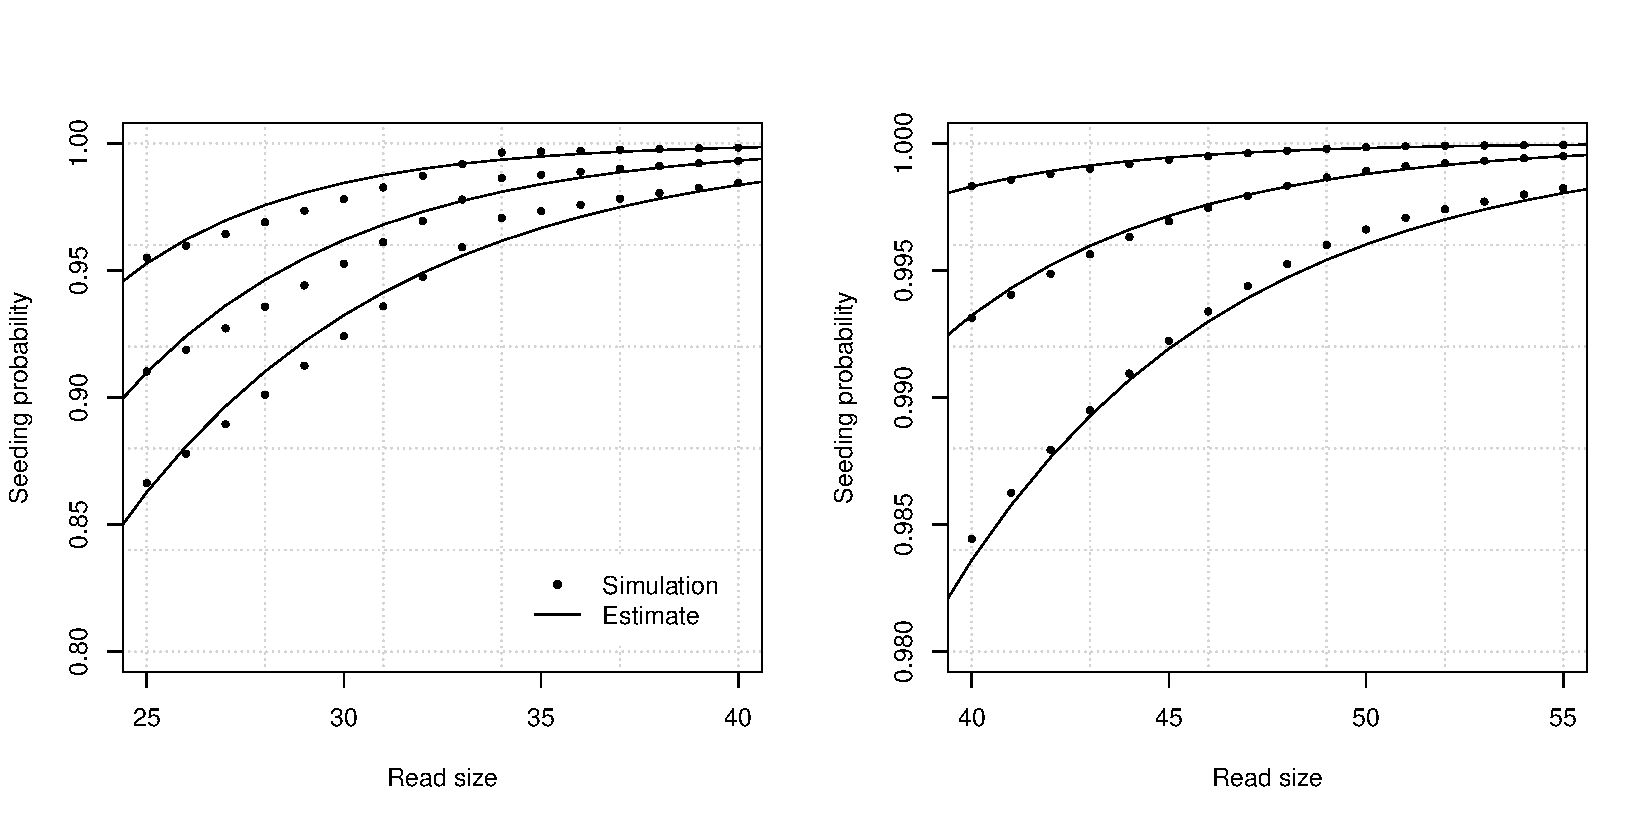
\includegraphics[scale=0.445]{simulp_short.pdf}
\caption{\textbf{Example worst case for seeding with substitutions only}.
The analytic combinatorics estimates of proposition~\ref{th:p} are
benchmarked against 10,000,000 random simulations. Shown on both panels
are the probablities that a read of given size contains a seed of size
$d=17$, either estimated by random simulations (dots), or by the estimate
derived in section~\ref{sec:substitutions}. The curves are drawn for
$p=0.005$, $p=0.010$ or $p=0.015$ (from top to bottom). The largest
difference between the estimates and the simulations is around $0.01$.}
\label{fig:illumina}
\end{figure}

Figure~\ref{fig:illumina} shows the accuracy of the estimates in one of
the worst cases. The curve is clearly distinct from the simulation at the
chosen scale, but the absolute difference is never higher than
approximately $0.01$ (and lower for read sizes above $40$). Whether this
error is acceptable depends on the problem. Very often, $p$ is known to
within approximately $0.01$, which is a more serious limitation on the
precision. In most practical applications, the approximation error of
proposition~\ref{th:ass} can be tolerated even in the worst case, but it
is important to bear in mind that it may not be totally negligible for
reads of size $50$ or lower.

If precision is crucial, remember that the exact solution can be found by
using all the singularities of the weighted generating function $S_\gamma$
(see remark~\ref{rem:exact}). If computatonal speed is an issue, the
singularities and associated proportionality constants can be precomputed
for a range of values of $p$ and $\gamma$.



\subsection{Oversimplified error models}

It is tempting to replace the somewhat complex error models of
sections~\ref{sec:deletions} and \ref{sec:insertions} by the uniform
subsitutions model of section~\ref{sec:substitutions} with an equivalent
error rate. An intuitive approach would be to set the only parameter
$q = 1-p$ of this model to the value of $q(1-\delta)$ of the more complex
ones, because those represent the probability of decoding a nucleotide
without error.

However, this approach is inaccurate because insertions and deletions can
have a strong influence. To show this, let us revisit
example~\ref{ex:num3} with an approximate substitution model instead of
the full error model.

\begin{example}
\label{ex:num4}
In example~\ref{ex:num3}, we computed the approximate probability that a
read of size $k=100$ contains no exact $17$-seed, where $p=0.05$,
$\delta=0.15$, $r=0.05$ and $\tilde{r}=0.45$. In such conditions, the
probability of decoding a nucleotide without error (given that it is not
in an insertion burst) is $(1-p-r)(1-\delta) =
0.765$. Now using a substitution model where $q = 0.765$ and thus $p =
0.235$, the analytic combinatorics estimate comes out as
$1.03726/1.002591^{101} \approx 0.79866$. This number is outside the 99\%
confidence $0.77373-0.77376$ and the uniform substitution model
underestimates the probability that the read contains a seed by more
than $2$ percentage points in this case.
\end{example}

The approximation error does not vanish. Actually, in the
conditions of example~\ref{ex:num4} it increases with the read size $k$.
Figure~\ref{fig:simulp_approx} shows the same data as
figure~\ref{fig:simulpins}, now fitted by an approximate substitution
error. The error can be as high as $5$ percentage points.


\begin{figure}[h]
\centering
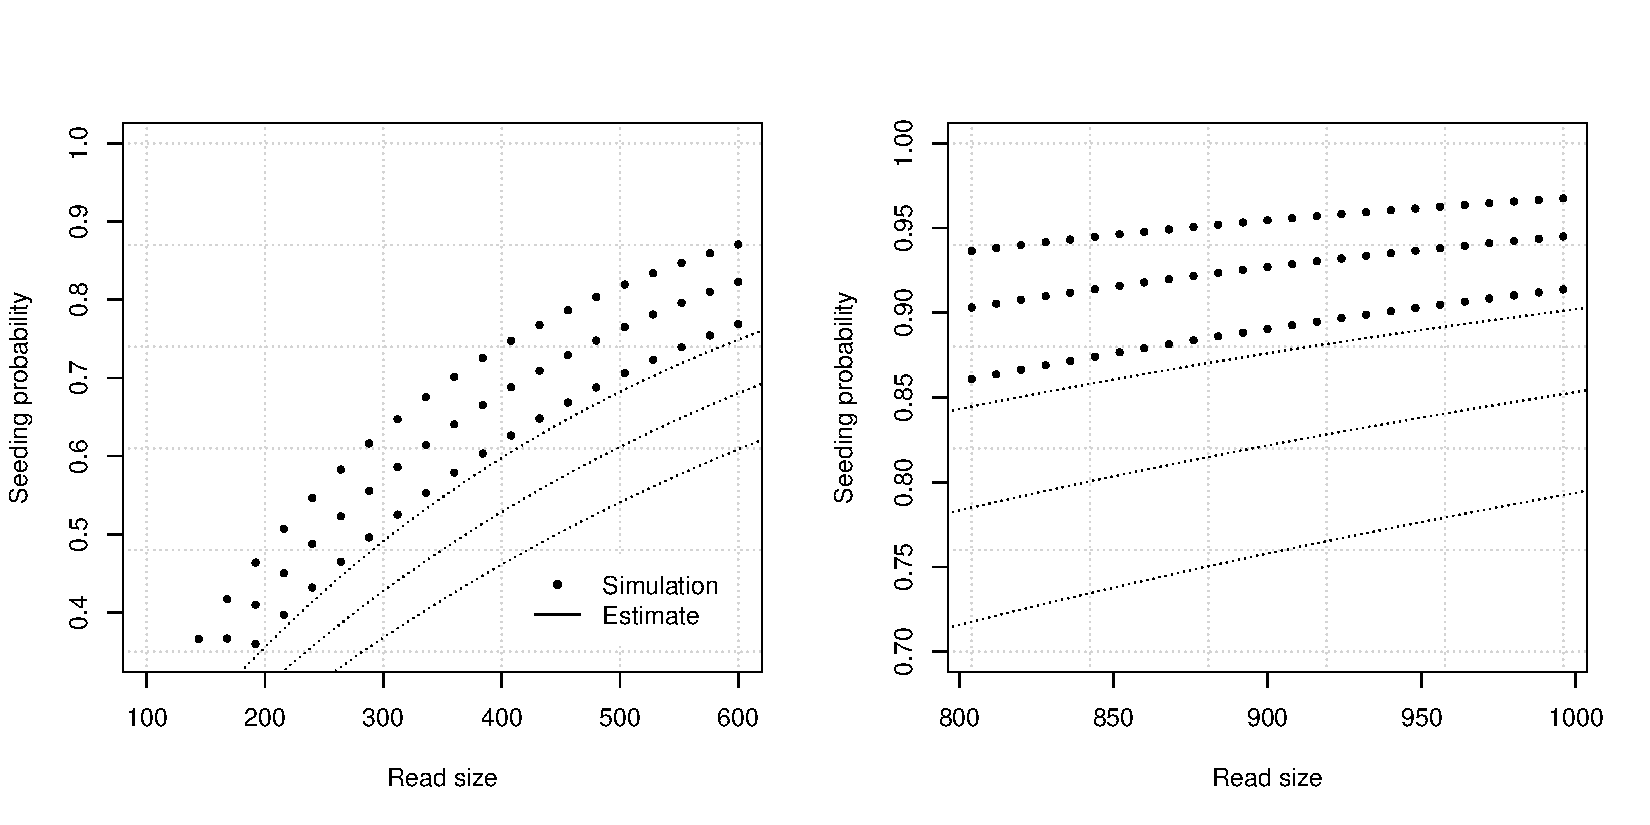
\includegraphics[scale=0.445]{simulp_approx.pdf}
\caption{\textbf{Example estimates with oversimplified error model}.
Shown on both panels are the probablities that a read of given size
contains a seed. The dots are obtained by 10,000,000 random simulations of
the full error model with $\gamma=17$, $p=0.05$, $\delta=0.15$, $\tilde{r}
= 0.45$ and $r=0.04$, $r=0.05$ or $r=0.06$ (from top to bottom); they
are the same as in figure~\ref{fig:simulp_approx}. The lines represent the
analytic combinatorics estimates of the oversimplified uniform
substitution model computed from proposition~\ref{th:p} with $p=0.2265$ or
$p=0.2350$ or $p=0.2435$ (top to bottom).}
\label{fig:simulp_approx}
\end{figure}

The conclusion is that the quality of the approximation collapses when
using approximate error models. One may argue that an error of 5
percentage points may be tolerable, but the actual amount of error when
using an approximate error model is unknown in genereal. Unsing simplified
error models is unsafe because convergence is slow (the probability that
the read contains a seed always tends to $1$ as the size increases) and
the error cannot be controlled.

Nevertheless, complexity comes at a cost. It is important to remember that
the parameters of the error model may be inaccurate, in which case the
error is also not controlled. If these parameters are hard to estimate, it
may be preferrable to use a simplified model. But in general, the amount
of data available in a sequencing run is sufficient to estimate the
parameters of the error model. In practice, the safest approach to compute
seeding probabilities is to use the full error model described in
section~\ref{sec:insertions} and estimate the four parameters from the
alignment data generated during the mapping. If $\delta$ or $r$
are small, they may be set to $0$ for simplicity, yielding the error
models of section~\ref{sec:deletions} or section~\ref{sec:substitutions}
(see remark~\ref{rem:russian_dolls}).







%%%%%%%%%%%%%%%%%% Inexact seeding %%%%%%%%%%%%%%%%%%%%%
\section{Advanced seeding methods}

Until now we have seen models of increasing complexity, but the transfer
graphs had a fixed layout, and the weighted generating functions were
ratios of polynomials of degree $\gamma$, the minimum size of the seed
(with the notable exception of the empirical error model, for which the
degree is not specified \textit{a priori}). In relation to different
problems, we will now explore other categories of models where the layout
of the transfer graph depends on $\gamma$, and where the degree of the
polynomials to solve will increase much faster than $\gamma$.

Because of this increased complexity, we will only consider the simplest
uniform substitution error model. Otherwise, the strategy remains
unchanged: we will formulate combinatorial problems, view their solutions
as walks on transfer graphs, encode these graphs as transfer matrices,
obtain the weighted generating functions of the solutions from
proposition~\ref{th:HBT} and approximate the answers using
proposition~\ref{th:ass}.

\subsection{Inexact seeds}

We now consider a more challenging problem. The ongoing development of
algorithms and data structures makes it possible to search inexact seeds,
\textit{i.e.} sequences that are very similar but not identical to the
target. This comes at a greater computational cost than finding exactly
similar sequences. If this cost is mitigated, it may be worth searching
inexact seeds because the chances are higher to identify the target.

The theory below is implemented within the framework of the uniform
substitution error model. Adaptations to more complex error models do not
present new theoretical challengnes, but the many cases to consider make
the models cumbersome, at the cost of concision and clarity. Let us begin
with a definition that will simplify the the following discussion.

\begin{definition}
A \textbf{single substitution interval} is a non-empty sequence of
nucleotides that cannot be extended left or right, and that contains at
most one substitution and no other error. An \textbf{inexact
$\gamma$-seed} is a single substitution interval of size $\gamma$ or
greater.
\end{definition}

We emphasize once more that our concern is the case of \emph{one}
substitution; the cases with more errors, or with errors of other types
are not considered. An exact $\gamma$-seed is an inexact $\gamma$-seed,
but the converse is not true. Figure~\ref{fig:sketchinexact} illustrates
the relationshiop between substitutions and single substitution intervals.
Note that single substitution intervals can overlap. In the models below,
this is something that we will have to account for explicitly.

\begin{figure}[h]
\centering
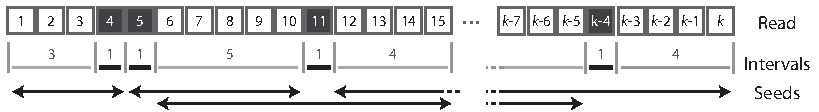
\includegraphics[scale=0.88]{sketch_inexact_seeding.pdf}
\caption{\textbf{Inexact seeding}. Substitutions (black squares) occur
uniformly at random within the read. They delimit $L$-blocks and single
substitution intervals. $L$-blocks consist of a substitution followed by
an error-free interval. There is always a substitution on the left of an
$L$-block, the error-free interval at the head of the read is
not an $L$-block. Single substitution intervals (arrows) are the longest
stretches of the read that contain at most one sbustitution.}
\label{fig:sketchinexact}
\end{figure}


We already computed the weighted generating function of reads under the
uniform substitutions model in section~\ref{sec:substitutions}. Namely, in
equation (\ref{eq:Rsub}) we found $R(z) = 1/(1-z) = 1 + z + z^2 + \ldots$
from which we concluded that the total weight of reads of size $k \geq 0$
is $1$. We now need to find the weighted generating function of reads that
do not contain an inexact $\gamma$-seed. For this, we introduce a new type
of combinatorial object.

\begin{definition}
An \textbf{$L$-block} is a substitution followed by an error-free
interval.
\end{definition}

The point of this definition is that a read is an error-free interval,
followed by a sequence of $L$-blocks. In a read without inexact
$\gamma$-seeds, not all the combinations of $L$-blocks are possible. For
instance, an $L$-block with $\gamma-2$ correct nucleotides can only be
followed by a substitution, \textit{i.e.} an $L$-block with $0$ correct
nucleotide (otherwise the concatenation of these two $L$-blocks forms an
inexact $\gamma$ seed). A substitution with $\gamma-3$ correct nucleotides
can be followed by an $L$-block with $0$ or $1$ correct nucleotide,
\textit{etc}.

\begin{figure}[h]
\centering
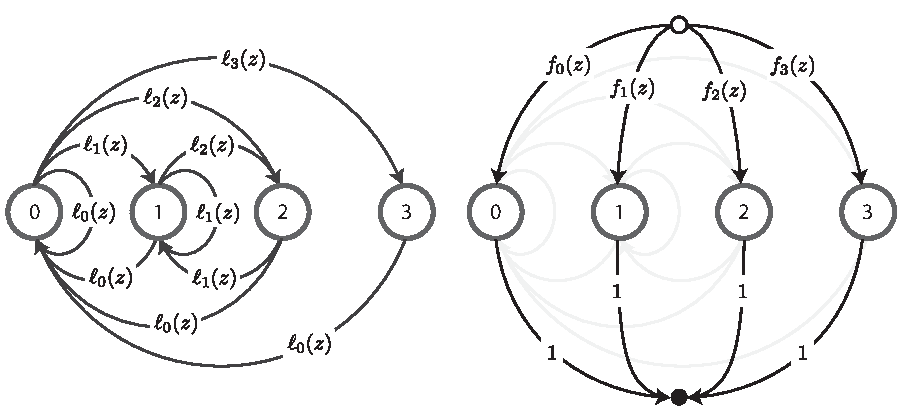
\includegraphics[scale=.79]{inexact_graph.pdf}
\caption{\textbf{Transfer graph of reads without inexact $5$-seeds}. Reads
are viewed as sequences of $L$-blocks. To not overload the figure, the
body of the transfer graph is shown on the left, and the head and tail
edges are shown on the right. The labels on the vertices represent the
number of correct nucleotides in the $L$-blocks. The terms $\ell_i(z)$ are
the weighted generating functions of $L$-blocks with $i$ correct
nucleotides for $i = 0,1,2,3$. The terms $f_i(z)$ are the weighted
generating functions of error-free intervals of size $i = 0,1,2,3$.}
\label{fig:inexact_graph}
\end{figure}

To give a concrete example, reads without inexact $5$-seeds can be seen as
walks on the graph shown in figure~\ref{fig:inexact_graph}. The numbers on
the vertices indicates the amount of correct nucleotides in an $L$-block.
There cannot be an $L$-block with $4$ or more correct nucleotides,
otherwise the read would contain an inexact $5$-seed. The edges capture
the relationships between consecutive $L$-blocks. The weighted generating
function of $L$-blocks with $i$ correct nucleotides is designated by
$\ell_i(z)$, for $i = 0, 1, 2, 3$.

The head and tail vectors are shown on the the right part of
figure~\ref{fig:inexact_graph}. Reads can start with up to $3$ correct
nucleotides. The weighted generating function of error-free intervals of
size $i$ is designated $f_i(z)$, for $i = 0, 1, 2, 3$. Finally, any
$L$-block can mark the end of the read, so all of them are connected to
the tail vertex by $1$, the weighted generating function of the the empty
oject $\varepsilon$. We do not need to connect the head and the tail node
with an such an edge, because as we will see below, the empty sequence is
already described by the transfer graph.

The weighted generating function of an $L$-block with $i$ correct
nucleotides is $\ell_i(z) = pz \times qz \times \ldots \times qz =
pz(qz)^i$, \textit{i.e.} the weighted generating function of a
substitution followed by $i$ correct nucleotides. In a similar way, the
weighted generating function of a stretch of $i$ correct nucleotides is
$f_i(z) = qz \times \ldots \times qz = (qz)^i$.

Because $f_0(z) = 1$, we now see that on the graph shown in
figure~\ref{fig:inexact_graph}, a walk starting from the head vertex and
going to the tail vertex through the vertex labelled $0$ has weighted
generating function $1$. This corresponds to the empty sequence, so there
is no need to add it again to the graph, so $\psi(z) = 0$.

In the general case $\gamma > 0$, the matrix of the body of the transfer
graph shown in figure~\ref{fig:inexact_graph} is

\begin{equation*}
M(z) = 
\begin{blockarray}{ccccccc}
       & \scriptstyle{0} & \scriptstyle{1} & \scriptstyle{2} &
    \ldots &  \scriptstyle{\gamma-3} & \scriptstyle{\gamma-2} \\
\begin{block}{c[cccccc]}
\scriptstyle{0} & pz  & pz(qz) & pz(qz)^2 & \ldots &
    pz(qz)^{\gamma-3} & pz(qz)^{\gamma-2} \\
\scriptstyle{1} & pz  & pz(qz) & pz(qz)^2 & \ldots &
    pz(qz)^{\gamma-3} & 0 \\
\scriptstyle{2} & pz  & pz(qz) & pz(qz)^2 & \ldots &
    0 & 0 \\
\vdots & \vdots  & \vdots & \vdots & \ddots & \vdots & \vdots  \\
\scriptstyle{\gamma-4} & pz  & pz(qz) & pz(qz)^2 & \ldots & 0 & 0 \\
\scriptstyle{\gamma-3} & pz  & pz(qz) & 0 & \ldots & 0 & 0 \\
\scriptstyle{\gamma-2} & pz  & 0      & 0 & \ldots & 0 & 0 \\
\end{block}
\end{blockarray}.
\end{equation*}


The head vector $H(z)$ is equal to $(1, qz, (qz)^2, \ldots,
(qz)^{\gamma-2})^\top$, the tail vector $T(z)$ is equal to $(1,1, \ldots,
1)^\top$, and $\psi(z) = 0$. By proposition~\ref{th:HBT}, the weighted
generating function of reads without an inexact seed can be computed as
$S_\gamma(z) = H(z) \cdot (I-M(z))^{-1} \cdot T(z)$.


\begin{example}
Let us revisit example~\ref{ex:num1}, where we approximated the
probability that a read of size $k=100$ has no seed for $\gamma=17$ and
for $p=0.1$; but this time we allow the seed to contain one substitution.
The matrix $M(z)$ has dimension $16$ and the weighted generating function
$S_{17}(z)$ can be written as $P(z)/Q(z)$, where $P$ and $Q$ are
polynomials. Using numerical methods to find the root of $Q$ with smallest
\textit{modulus}, we obtain $z_1 \approx 1.079244$. Likewise, we obtain
$-P(z_1)/Q'(z_1) \approx 2.326700$, so the probability that the read does
not contain an inexact seed is approximately $2.326700/1.079244^{101}
\approx 0.0010511$. For comparison, a 99\% confidence interval obtained by
performing 10 billion random simulations is $0.001049-0.001054$.
% The magic number is 1051660 out of 10 billion.
In the same conditions, the chances that the read contains an exact seed
was 90.4\%, compared to 99.9\% when one substitution is allowed.
\end{example}

The approximations have the typical accuracy of analytic combinatorics
estimates. Figure~\ref{fig:simulpinexact} shows the precision of the
estimates for different values of the substitution rate $p$ and the read
size $k$. Observe that the probability that the read contains an inexact
seed is substantially higher than the probability that it contains an
exact seed (compare with figure~\ref{fig:simulp}). This means that
efficient algorithms to find inexact seeds can greatly reduce the number
of false negatives in the mapping problem.


\begin{figure}[h]
\centering
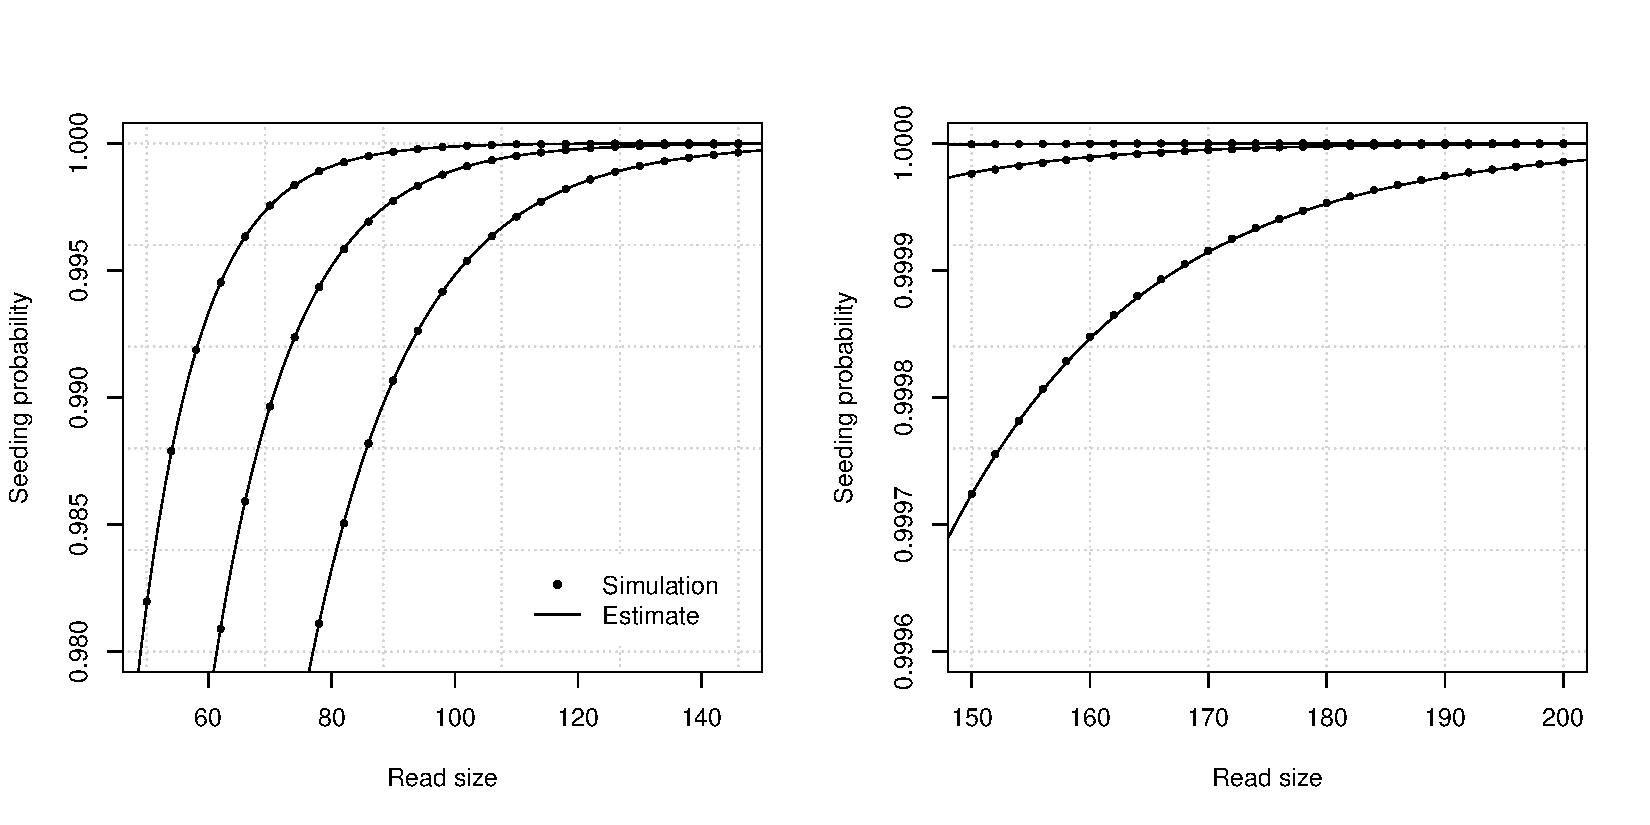
\includegraphics[scale=0.445]{simulp-inexact.pdf}
\caption{\textbf{Example estimates for inexact seeding with substitutions
only}. The analytic combinatorics estimates described in this section
are benchmarked against random simulations.  Shown on both panels are the
probablities that a read of given size contains an inexact seed, either
estimated by random simulations (dots), or by the method described above
(lines). The curves are drawn for $\gamma=17$, $p=0.08$, $p=0.10$ or
$p=0.12$ (from top to bottom). 10,000,000 simulations are run on the left
panel and 100,000,000 on the right one.}
\label{fig:simulpinexact}
\end{figure}


Unfortunately, the expressions of the weighted generating functions given
by proposition~\ref{th:HBT} are very cumbersome, and they may take hours
to evaluate. For instance, the degrees of $P$ and $Q$ for $\gamma=17$ are
$152$ and $153$, respectively.

The best option here is to pre-compute the dominant singularities and
associated multiplicative constants for a useful range of values of
$\gamma$ (up to $30$ is sufficient for most applications) and of the
parameter $p$ (up to $0.25$ is sufficient for most application). Once
these values are stored, the estimates can be calculated rapidly.






%%%%%%%%%%%%%%%%%% False positives %%%%%%%%%%%%%%%%%%%%%
\subsection{Type I errors}
\label{sec:fp}


Our concern so far was whether reads contain a seed, \textit{i.e.} an
error-free (or almost free) interval of sufficient size. If this is the
case, the target sequence is among the candidates and we implicitly assume
that it will be identified as the best hit during the alignment stage.
But we did not discuss what happens if the read does not contain a seed.

There are two possible cases. The first is that the mapping procedure
returns no hit. The conclusion is then that the sequence does not belong
to the genome, or that it cannot be mapped. In analogy with statistical
testing, we will call this a ``type II error''. The second case is that
the mapping procedure returns a hit. This cannot be a true hit because the
target was discarded during the seeding stage. We will call this a ``type
I error''. Type I errors are the most difficult to detect, because nothing
distinguishes them from true hits, at least at the seeding stage.

It is important to emphasize that in this version of the mapping problem,
the split between type I and type II errors amounts to the probability
that the read contains no seed (because we assume that all the candidates
are aligned and that the alignment always identifies the true hit when it
is present among the candidates). This split depends on the genome, and
more particularly on the configuration of its repeated sequences. A
stretch of  $\gamma$ nucleotides matches a random genome with probability
$O(4^{-\gamma})$. However, genomes are not a succession of random
nucleotides. Large sequences are often duplicated, to the extent that the
greater part of eukaryotic genomes can be considered repetitive. In
addition, repeats are usually not exactly identical, but only similar.
This means that the $O(4^{-\gamma})$ term can be a spectacular
underestimate.

A complete treatment of type I errors is presently not possible. We will
focus on a single case that will be the basis for further development.
More specifically, we will assume that the target sequence has exactly one
duplicate in the genome, and that they differ from each other only by
uniform substitutions (we will see below how to relax these assumptions).
The problem then amounts to finding the probability that the seeding
process identifies the duplicate as a candidate, but not the target
sequence. Figure~\ref{fig:example_typeI} shows how this can occur.

\begin{figure}[h]
\centering
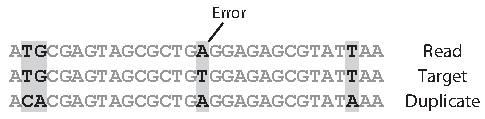
\includegraphics[scale=1]{example_typeI.pdf}
\caption{\textbf{Example type I error}. A read of $30$ nucleotides
contains a single error at the sixteenth position. The erroneous
nucleotide is identical to the duplicate sequence at this position. This
creates a match of $24$ nucleotides for the duplicate sequence, while the
longest match for the target is $15$ nucleotides. Thus, using seeds of
size greater than $15$ would result in a type I error (even though the
duplicate has three differences with the read and the target has only
one).}
\label{fig:example_typeI}
\end{figure}

\begin{remark}
With only one reference sequence, ``error-free'' and ``matching''
nucleotides are the same. With more than one reference, we must take care
of distinguishing them. In this case, matching nucleotides can be
incorrect (they can match the wrong sequence).
\end{remark}

Instead of tackling this problem directly, we will set a more general
framework where a read can match two similar sequences denoted $(+)$ and
$(-)$. A read now consists of four types of nucleotides: those matching
both sequences, those matching the $(+)$ sequence only, those matching the
$(-)$ sequence only, and those matching none. The first type will be
referred to as a \emph{match} and the last three as \emph{mismatches}
(single or double). The following definitions will be useful to sketch
the transfer graph.

\begin{definition}
An \textbf{$R$-block} is a mismatch-free interval followed by a single or
a double mismatch. A \textbf{$(+)$ interval} (respectively \textbf{$(-)$
interval}) is a sequence of nucleotides matching the $(+)$ sequence
(respectively $(-)$ sequence) that cannot be extended left or right. A
\textbf{$(+)$ seed} (respectively \textbf{$(-)$ seed}) is a $(+)$ interval
(respectively $(-)$ interval) of size $\gamma$ or greater.
\end{definition}

This information is summarized in figure~\ref{fig:sketchdual}. We will use
it to find a construction for reads without either $(+)$ or $(-)$ seeds.
We will later show how this can be used to find the probabilities of type
I errors.

\begin{figure}[h]
\centering
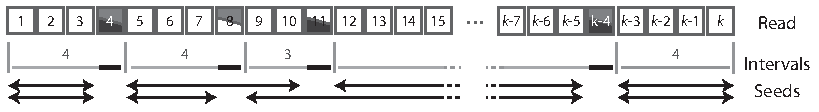
\includegraphics[scale=0.88]{sketch_dual_mutations.pdf}
\caption{\textbf{Seeding with two reference sequences}.
Matches are represented as white squares, mismatches against the $(+)$
sequence as bottom black wedges, mismatches against the $(-)$ sequence as
top black wedges, and double mismatches as black squares. They delimit
$R$-blocks consisting of mismatch-free intervals followed by a mismatch.
The last nucleotide of an $R$-block is always a mismatch so the
mismatch-free interval at the tail of the read is not an $R$-block. $(+)$
or $(-)$ intervals are stretches of the read that match either the $(+)$
sequence (top arrow) or the $(-)$ sequence (bottom arrow) and that cannot
be extended left or right.}
\label{fig:sketchdual}
\end{figure}

\begin{remark}
When a subsequence is both a $(+)$ and a $(-)$ seed (the head and the tail
of the read shown in figure~\ref{fig:sketchdual} for instance), then both
sequences are candidates.
\end{remark}

Reads can be viewed as sequences of $R$-blocks followed by a mismatch-free
interval. Reads without $(+)$ or $(-)$ seeds have particuarly complex
constraints on the arrangements of those $R$-blocks. For instance, an
$R$-block of size $\gamma$ (\textit{i.e.} $\gamma-1$ matches followed by a
mismatch) must be followed by a mismatch if the final nucleotide is a
single mismatch, but it can be followed by up to $\gamma-1$ matches if the
last nucleotide is a double mismatch.

To give a concrete example, we will consider reads without $(+)$ or $(-)$
seeds of size $3$. The read below features two matches, followed by a
double mismatch, followed by a mismatch against the $(-)$ sequence. The
numbers between brackets $(0,1)$ indicate the respective amount of
nucleotides matching the $(-)$ and the $(+)$ sequences at the end of the
$R$-block. At that point, there are only five possiblities for the next
$R$-block; every other combination would create a $(+)$ seed or a $(-)$
seed.

\begin{inset}
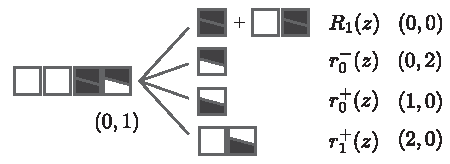
\includegraphics[scale=0.9]{example_dual.pdf}
\end{inset}

Appending a double mismatch or a match followed by a double mismatch (top
case) brings the number of nucleotides matching $(-)$ and $(+)$ at the end
of the $R$-block to $(0,0)$. The weighted generating function of this
union of $R$-blocks is denoted $R_1(z)$. Appending a mismatch against the
$(-)$ sequence (second case from the top), \textit{i.e.} an $R$-block with
weighted generating function $r_0^-(z)$ brings the amount of matching
nucleotides to $(0,2)$. Conversely, appending a mismatch against the $(+)$
sequence (third case from the top), \textit{i.e.} an $R$-block with
weighted generating function $r_0^+(z)$ brings the amount of matching
nucleotides to $(1,0)$. Finally, appending a match followed by a mismatch
against the $(+)$ sequence (bottom case), \textit{i.e.} an $R$-block with
weighted generating function $r_1^+(z)$ brings the amount of matching
nucleotides to $(2,0)$.


By considering all the cases, we obtain the transfer graph shown in
figure~\ref{fig:graph_fp}. Even for such a small value of $\gamma$, the
graph is so dense that the edges have been separated in two panels and
encoded as symbols in order to not overload the figure.

\begin{figure}[h]
\centering
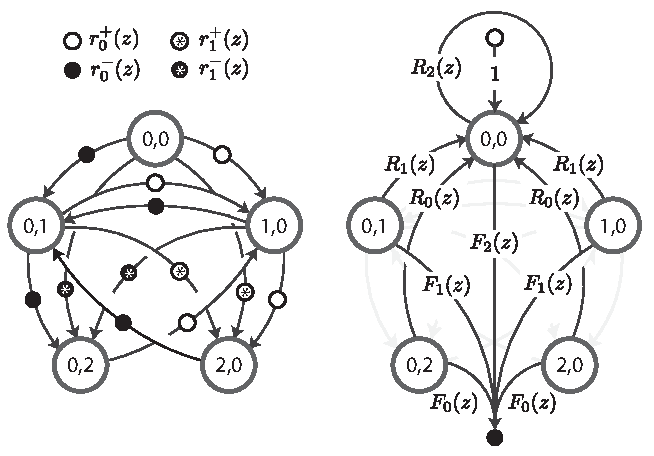
\includegraphics[scale=1]{false_positives_graph.pdf}
\caption{\textbf{Transfer graph of reads without seed of size $3$ for
either $(+)$ or $(-)$}. Reads can match two sequences referred to as $(+)$
and $(-)$. They are viewed as sequences of $R$-blocks. To not overload the
figure, the edges are split between the left and right panels. The labels
on the vertices represent the respective sizes of the $(-)$ and $(+)$
intervals at the end of an $R$-block. NEEDS REWRITING. Weighted generating
functions $r_i^+(z)$ represent $R$-blocks with $i$ matches and terminated
by a mismatch against the $(+)$ sequence (symmetrically for the $(-)$
sequence). Weighted generating function $R_i(z)$ represent $R$-blocks with
\emph{up to} $i$ matches and terminated by a double mismatch. Weighted
generating functions $F_i(z)$ represent mismatch-free intervals of
\emph{up to} $i$ matches.}
\label{fig:graph_fp}
\end{figure}

As in the example above, the numbers in the vertices indicate the amount
of nucleotides matching $(-)$ and $(+)$ at the end of the $R$-blocks.
Since $R$-blocks are terminated by a mismatch, at least one of these
numbers is $0$. The body of the transfer graph is only partially
represented on the left panel. The edges pointing to the vertex $(0,0)$
are displayed on the right panel, together with the head and tail edges.
The four kinds of edges on the left panel correspond to different
$R$-blocks with weighted generating functions $r_0^+(z)$, $r_0^-(z)$,
$r_1^+(z)$ and $r_1^-(z)$. The sign indicates which sequence is
\emph{mismatched} at the end of the $R$-block and the index is the number
of matches in the $R$-block.

The edges of the body of the transfer graph on the right panel point to
the vertex $(0,0)$. All the vertices are connected to this vertex because
appending an $R$-block terminated by a double mismatch always brings the
read to this state. The weighted generating functions $R_0(z)$, $R_1(z)$
and $R_2(z)$ represent such $R$-blocks with \emph{up to} $0$, $1$ or $2$
matches, respectively.

In the initial state of the read, the amount of matching nucleotides is
$(0,0)$, which is indicated by the label $1$ on the edge between the head
vertex and the vertex $(0,0)$. This is equivalent to prepending the read
by the empty object $\varepsilon$. Reads are terminated by a sequence of
matches. The weighted generating functions $F_0(z)$, $F_1(z)$ and $F_2(z)$
represent mismatch-free intervals of size \emph{up to} $0$, $1$ or $2$,
respectively. Here $\psi(z) = 0$. The empty sequence is present in the
graph (take a path from the head vertex to the tail vertex through $(0,0)$
with no match appended at the tail), and no extra sequence needs to be
added.

The same logic can be applied for higher values of $\gamma$. The transfer
graph becomes too cumbersome to represent but the transfer matrix has
enough regularity to be specified in full. The general transfer matrix
associated with the body of the transfer graph has dimension $2\gamma-1$
and is defined as


\begin{equation*}
M(z) =
\begin{blockarray}{cccccccc}
   & \scriptstyle{0,0} & \scriptstyle{1,0} & 
    \ldots & \scriptstyle{\gamma-1,0} &
    \scriptstyle{0,1} & \ldots &
    \scriptstyle{1,\gamma-1}\\
\begin{block}{c[ccccccc]}
\scriptstyle{0,0} & R_{\gamma-1}(z)  & r_0^+(z) & \ldots &
    r_{\gamma-2}^+(z) & r_0^-(z) & \ldots & r_{\gamma-2}^-(z) \\
\scriptstyle{1,0} & R_{\gamma-2}(z) \\
\scriptstyle{2,0} & R_{\gamma-3}(z) \\
\vdots & \vdots & & A(z) & & & B(z) \\
\scriptstyle{\gamma-1,0} & R_0(z) \\
\scriptstyle{0,1} & R_{\gamma-1}(z) \\
\scriptstyle{0,2} & R_{\gamma-2}(z) \\
\vdots & \vdots & & C(z) & & & D(z) \\
\scriptstyle{0,\gamma-1} & R_0(z) \\
\end{block}
\end{blockarray},
\end{equation*}
where $A(z)$, $B(z)$, $C(z)$ and $D(z)$ are square matrices with dimension
$\gamma-1$ and defined as

\begin{equation*}
A(z) = 
\begin{blockarray}{cccccc}
   & \scriptstyle{1,0} & \scriptstyle{2,0} & \ldots &
    \scriptstyle{\gamma-2,0} & \scriptstyle{\gamma-1,0} \\
\begin{block}{c[ccccc]}
\scriptstyle{1,0} & 0 & r_0^+(z) & \ldots &
    r_{\gamma-3}^+(z) & r_{\gamma-2}^+(z) \\
\scriptstyle{2,0} & 0 & 0 & \ldots &
    r_{\gamma-4}^+(z) & r_{\gamma-3}^+(z) \\
\vdots & \vdots & \vdots & \ddots & \vdots & \vdots \\
\scriptstyle{\gamma-2,0} & 0 & 0 & \ldots & 0 & r_0^+(z) \\
\scriptstyle{\gamma-1,0} & 0 & 0 & \ldots & 0 & 0 \\
\end{block}
\end{blockarray},
\end{equation*}

\begin{equation*}
B(z) = 
\begin{blockarray}{cccccc}
   & \scriptstyle{0,1} & \scriptstyle{0,2} & \ldots &
    \scriptstyle{0,\gamma-2} & \scriptstyle{0,\gamma-1} \\
\begin{block}{c[ccccc]}
\scriptstyle{1,0} & r_0^-(z) & r_1^-(z) & \ldots &
    r_{\gamma-3}^-(z) & r_{\gamma-2}^-(z) \\
\scriptstyle{2,0} & r_0^-(z) & r_1^-(z) & \ldots &
    r_{\gamma-3}^-(z) & 0 \\
\vdots & \vdots & \vdots & \ddots & \vdots & \vdots \\
\scriptstyle{\gamma-2,0} & r_0^-(z) & r_1^-(z) & \ldots & 0 & 0 \\
\scriptstyle{\gamma-1,0} & r_0^-(z) & 0 & \ldots & 0 & 0 \\
\end{block}
\end{blockarray},
\end{equation*}

\begin{equation*}
C(z) = 
\begin{blockarray}{cccccc}
   & \scriptstyle{1,0} & \scriptstyle{2,0} & \ldots &
    \scriptstyle{\gamma-2,0} & \scriptstyle{\gamma-1,0} \\
\begin{block}{c[ccccc]}
\scriptstyle{0,1} & r_0^+(z) & r_1^+(z) & \ldots &
    r_{\gamma-3}^+(z) & r_{\gamma-2}^+(z) \\
\scriptstyle{0,2} & r_0^+(z) & r_1^+(z) & \ldots &
    r_{\gamma-3}^+(z) & 0 \\
\vdots & \vdots & \vdots & \ddots & \vdots & \vdots \\
\scriptstyle{0,\gamma-2} & r_0^+(z) & r_1^+(z) & \ldots & 0 & 0 \\
\scriptstyle{0,\gamma-1} & r_0^+(z) & 0 & \ldots & 0 & 0 \\
\end{block}
\end{blockarray},
\end{equation*}

\begin{equation*}
D(z) = 
\begin{blockarray}{cccccc}
   & \scriptstyle{0,1} & \scriptstyle{0,2} & \ldots &
    \scriptstyle{0,\gamma-2} & \scriptstyle{0,\gamma-1} \\
\begin{block}{c[ccccc]}
\scriptstyle{0,1} & 0 & r_0^-(z) & \ldots &
    r_{\gamma-3}^-(z) & r_{\gamma-2}^-(z) \\
\scriptstyle{0,2} & 0 & 0 & \ldots &
    r_{\gamma-4}^-(z) & r_{\gamma-3}^-(z) \\
\vdots & \vdots & \vdots & \ddots & \vdots & \vdots \\
\scriptstyle{0,\gamma-2} & 0 & 0 & \ldots & 0 & r_0^-(z) \\
\scriptstyle{0,\gamma-1} & 0 & 0 & \ldots & 0 & 0 \\
\end{block}
\end{blockarray}.
\end{equation*}


As per proposition~\ref{th:HBT}, the weighted generating function of reads
with no $(+)$ nor $(-)$ seeds is given by $H(z)^\top \cdot (I-M(z))^{-1}
\cdot T(z)$. In this case the head vector $H(z)$ is equal to
$(1,0,0,\ldots,0)^\top$ and the tail vector $T(z)$ is equal to
$(R_{\gamma-1}(z), R_{\gamma-2}(z), \ldots, R_0(z), R_{\gamma-2}(z),
\ldots, R_0(z))^\top$.

Under the assumption that mismatches occur uniformly in the read,
nucleotides of each type occur with probabilities $a$, $b$, $c$ or $d$,
with $a+b+c+d=1$, where $a$ is the probability that the nucleotide is a
double match, $b$ that it is a mismatch against $(+)$, $c$ that it is a
mismatch against $(-)$ and $d$ that it is a mismatch against both. With
these notations we obtain

\begin{equation}
\label{eq:abcd}
\begin{gathered}
r_i^+(z) = (az)^icz, \\
r_i^-(z) = (az)^ibz, \\
R_i(z) = \big( 1 + az + \ldots + (az)^i \big)dz, \\
F_i(z) = 1 + az + \ldots + (az)^i.
\end{gathered}
\end{equation}

We could now find the weighted generating function of the reads without
$(+)$ or $(-)$ seeds, but we will return to the original problem of
computing the probability of a type I error. In this context, the $(+)$
sequence is the target and the $(-)$ sequence is the duplicate.


We will assume that each nucleotide is decoded incorrectly with
probability $p$ and that for each nucleotide, the duplicate sequence
differs from the target with probability $\kappa$. A nucleotide is a
mismatch for both sequences if it is a read error (probability $p$) and if
either the duplicate is identical to the target (probability $1-\kappa$)
or it is different from both the target and the decoded nucleotide
(probability $2\kappa/3$). The other probabilities can be computed with
similar arguments, yielding $a = (1-p)(1-\kappa)$, $b = p\kappa/3$, $c =
(1-p)\kappa$ and $d = p(1-\kappa/3)$.

The model is completely specified by $p$ and $\kappa$. With their actual
values at hand, we can use proposition~\ref{th:ass} to obtain an
asymptotic estimate of the probability that a read has no match for the
target \emph{and} no match for the duplicate. Call this estimated
probability $P_2$. Using the results of section~\ref{sec:substitutions},
we can also compute an asymptotic estimate of the probability that the
read does not contain an exact $\gamma$-seed (irrespective of potential
matches to the duplicate). Call this estimated probability $P_1$. We can
thus estimate the probability that the read contains a match of size
$\gamma$ or greater for the duplicate sequence \emph{but} no exact
$\gamma$-seed as $P_1 - P_2$.

\begin{example}
\label{ex:num5}
Let us approximate the probability of type I error (with one duplicate)
for a read of size $k=100$ with $\gamma=17$ and for substitution rates
$p=0.10$ and $\kappa=0.10$. In example~\ref{ex:num1} we found $P_1 \approx
1.396145 / 1.0268856^{101}$. To compute $P_2$, we substitute $a=0.81,
b=0.09, c=0.00333, d=0.09667$ in the expression of the $33 \times 33$
transfer matrix $M(z)$ and in the expression of $T(z)$. We then compute
the expression $H(z)^\top \cdot (I-M(z))^{-1} \cdot T(z)$ and obtain a
function $P(z)/Q(z)$ where $P$ and $Q$ are polynomials of degree $288$ and
$289$, respectively. The root of $Q$ with smallest \textit{modulus} is the
dominant singularity $z_1$ of the weighted generating function. Using
numerical approaches, we find $z_1 \approx 1.0272930245$. We compute the
proportionality constant of proposition~\ref{th:ass} as $P(z_1)/Q'(z_1)
\approx 1.4032791$ from which we obtain $P_2 \approx
1.4032791/1.0272930245^{101}$. The type I error rate is then approximately
equal to $0.0032906$. For comparison, a 99\% confidence interval obtained
by performing 10 billion random simulations is $0.003288-0.003292$.
% The magic number is 32900981 out of 10 billion.
\end{example}

Figure~\ref{fig:simulp_fp} illustrates the precision of this estimate for
different values of the substitution rate $\kappa$ and of the read size
$k$. Observe that the estimates are accurate even for such low probability
of occcurrence.


\begin{figure}[h]
\centering
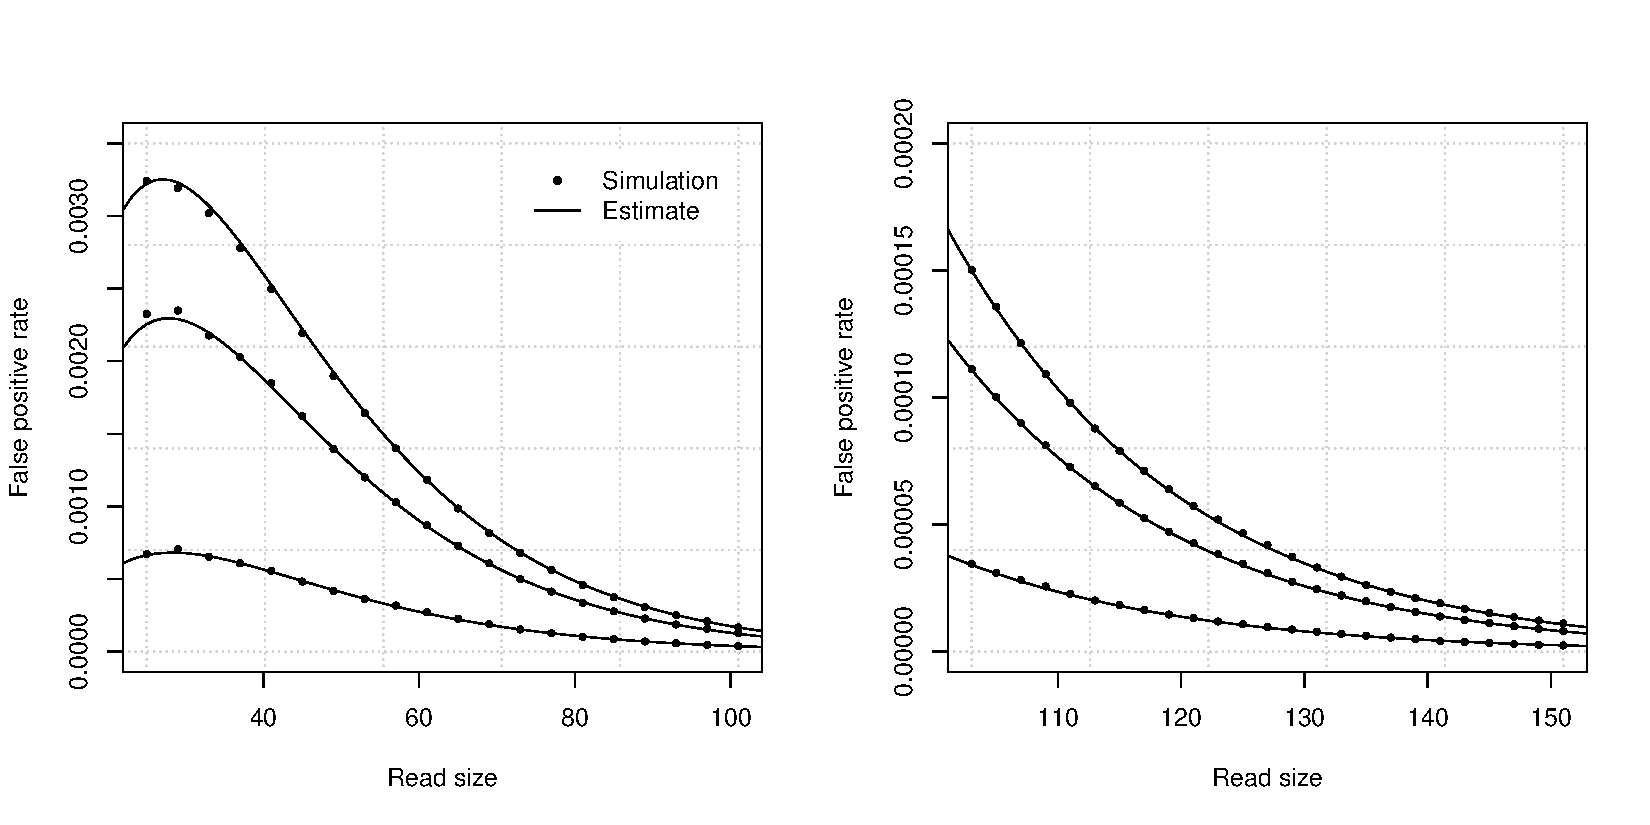
\includegraphics[scale=0.445]{simulp_false_positives.pdf}
\caption{\textbf{Example estimates of type I errors (one
duplicate)}. The analytic combinatorics estimates are benchmarked against
random simulations. Shown on both panels are the probablities that a read
of given size will give a type I error, either estimated by 10,000,000
(left) or 100,000,000 (right) random simulations (dots), or by the method
described above (lines). The curves are drawn for $\gamma=17$ and
$p=0.05$, $\kappa=0.05$, $\kappa=0.15$ or $\kappa=0.25$ (from top to
bottom).}
\label{fig:simulp_fp}
\end{figure}

Computing $P_2$ with proposition~\ref{th:ass} requires finding a weighted
generating function $P(z)/Q(z)$ where $P$ and $Q$ are polynomials with too
many terms to fit in this document. It is thus problematic to compute the
approximations efficiently. The best option is once again to pre-compute
the dominant singularities and associated multiplicative constants for a
useful range of $\gamma$ (up to $30$ is sufficient for most applications)
and of the parameters $p$ and $\kappa$ (up to $0.25$ is sufficient for
most applications). Once these values are stored, the estimates can be
calculated rapidly without having to compute the weighted generating
function and finding its dominant singularity.

We have started this section with the assumption that the target has
exaclty one duplicate. Also, $\kappa$ is usually unknown so how are the
estimates derived above useful?

First, it is important to stress that the seeding strategy is efficient
only when the target has few duplicates. Some sequences have more than
100,000 copies in the human genome. In such cases, the seeding process
yields many candidates that will cost time at the alignment stage, for in
the end relatively small chances of identifying the correct target. As a
consequence, most mapping algorithms bail out as soon as they gather
enough evidence that the target has many duplicates. There is thus little
incentive to develop accurate estimates of type I error for highly
repeated sequences, and one should focus on the case of intermediate
amount of repeats, say around 20.

We can extend the theory developed above to more than one duplicate. The
probability that a read contains no match for the duplicate given that it
contains no match for the target is $P_2 / P_1$. If the target has $N$
extra duplicates evolving independently with mutation rate $\kappa$, the
probability that a read contains no match for any of the duplicates given
that it contains no match for the target is $(P_2 / P_1)^N$. The
probability of a type I error is thus $P_1\big(1-(P_2 / P_1)^N\big)$. For
$N=1$, we recover $P_1-P_2$ and for large $N$, the value approaches $P_1$,
the probability that the read has no seed.

This approach is somewhat naive because repeated sequences do not evolve
independently of each other and $N$ is usually unknown. However, it gives
a handle on the problem as $N$ and $\kappa$ can be estimated during the
seeding or better, stored for every position of the genome.

Also observe that the case of one duplicate gives a lower bound for the
probability of type I error. When there is exactly one duplicate, type I
errors are almost impossible to detect because the mapping process
identifies a single hit that is similar to the read (as if a seed was
present and the target had no duplicate). If the proportion of the genome
that is repeated is $x$ and $P^*$ is the maximum of $P_1-P_2$ relative to
unknown $\kappa$, then $xP^*$ is a reasonable lower bound on the
probability of type I errors. If more information about the read, or about
the seeding and alignment processes is available, then this lower bound
can vary.





\subsection{MEM seeds}

In the exact seeding scheme considered so far, every subsequence of the
genome that matches $\gamma$ consecutive nucleotides of the read is
considered a candidate. While assuring good chances of discovering the
target, this approach often yields ``too many'' useless candidates, which
costs computational time at the alignment stage. An alternative scheme
called MEM seeding (Maximal Exact Match) gives better empirical results.
The principle is to use as seeds only the longest local matches between
the read and the genome.

\begin{definition}
A $\gamma$-MEM (Maximal Exact Match) is a sequence of at least $\gamma$
nucleotides from the read, that matches a subsequence of the genome and
that cannot be extended left or right.
\end{definition}

\begin{remark}
Note that error-free intervals and mismatch-free intervals are disjoint,
whereas MEMs can be overlapping (and usually are).
\end{remark}

Since there are fewer MEM seeds than exact $\gamma$-seeds, MEM seeding is
more prone to errors than exact seeding. As we will see below, an
important difference is that the combined frequencies of type I and type
II errors is strictly greater than the probability that the read contains
an error-free interval of size $\gamma$ or greater.


To make the problem more concrete, we will consider as in
section~\ref{sec:fp} that the target has exactly one duplicate sequence.
In a similar way, we will start by defining two potential matches referred
to as $(+)$ and $(-)$. The definitions of $R$-block, $(+)$ interval and
$(-)$ interval given in section~\ref{sec:fp} still apply.


\begin{figure}[h]
\centering
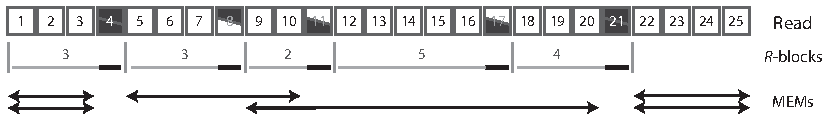
\includegraphics[scale=0.88]{sketch_MEM.pdf}
\caption{\textbf{MEMs (with two references)}. The symbols are the
same as in figure~\ref{fig:sketchdual}. Matches are represented as white
squares, mismatches for the $(+)$ sequence as bottom black wedges,
mismatches for the $(-)$ sequence as top black wedges, and double
mismatches as black squares. They delimit $R$-blocks consisting of
mismatch-free intervals followed by a mismatch. The last nucleotide of
an $R$-block is always a mismatch so the mismatch-free interval at the
tail of the read is not an $R$-block. MEMs (arrows) are stretches of the
read that match any of the two sequences and that cannot be extended left
or right. MEMs matching the $(+)$ sequence are represented at the top and
MEMs matching the $(-)$ sequence at the bottom. In this example, the
central stretch of $5$ nucleotides matching the $(+)$ sequence is not used
as seed because it is included in a stretch of $12$ nucleotides matching
the $(-)$ sequence.}
\label{fig:sketchmem}
\end{figure}

Figure~\ref{fig:sketchmem} highlights the properties of MEMs. Notice how a
match for $(+)$ is masked by a longer match for $(-)$. Nucleotides from 12
to 16 match the $(+)$ sequence, creating a potential seed. However, it is
contained in a match for the $(-)$ sequence from nucleotides 9 to 20.
Since the match for $(+)$ is not a MEM, it is not used as a seed. Cases
such as this one can cause type I errors to occur even when the reads
contains matches of size $\gamma$ or greater for the target.

\begin{remark}
When a MEM matches both sequences (the head and the tail of the read shown
in figure~\ref{fig:sketchmem} for instance), then both sequences are
candidates.
\end{remark}


As in section~\ref{sec:fp}, reads are seen as sequences of $R$-blocks. We
will first focus on the probability that a read does not contain a
$\gamma$-MEM seed for the $(+)$ sequence, from which we will later deduce
the probabilities of type I and type II errors. This restriction imposes
relatively complex constraints on the $R$-blocks. For instance, an
$R$-block of size $\gamma$ (\textit{i.e.} $\gamma-1$ matches followed by a
mismatch) must be followed by a mismatch if the final nucleotide is a
mismatch for the $(-)$ sequence, but it may be followed by up to
$\gamma-1$ matches if this nucleotide is a double mismatch, or by any
number of matches if it is a mismatch for the $(+)$ sequence.


To give a concrete example, we will consider $\gamma$-MEMs of size $3$.
The read below features two matches, followed by a double mismatch,
followed by a mismatch for the $(+)$ sequence. The symbols between
brackets $(*,0)$ indicate the respective amount of nucleotides matching
the $(-)$ and the $(+)$ sequences at the end of the $R$-block. All the
$R$-blocks terminated by a mismatch against the $(+)$ sequence are
equivalent because the subsequent $R$-block cannot be part of a
MEM for the $(+)$ sequence. So the only information we need regarding the
$(-)$ sequence is whether this amount is greater than $0$, which we
represent by the $*$ symbol. At that point, there are infinitely many
possiblities for the next $R$-blocks, but only four distinct classes do
not create a MEM seed for the $(+)$ sequence.

\begin{inset}
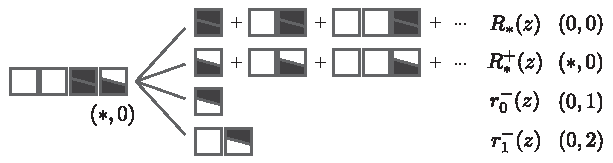
\includegraphics[scale=0.9]{example_dual_mem.pdf}
\end{inset}

Appending any number of matches followed by a double mismatch (top case)
brings the number of nucleotides matching $(-)$ and $(+)$ at the end of
the $R$-block to $(0,0)$. The weighted generating function of this union
of $R$-blocks is denoted $R_*(z)$. Appending any number of matches
followed by a mismatch against the $(+)$ sequence (second case from the
top) maintains the amount of matching nucleotides as $(*,0)$. The weighted
generating function of this union of $R$-blocks is denoted $R_*^+(z)$.
Appending a mismatch for the $(-)$ sequence (third case from the top),
\textit{i.e.} an $R$-block with weighted generating function $r_0^-(z)$
brings the amount of matching nucleotides to $(0,1)$. Finally, appending a
match followed by a mismatch for the $(-)$ sequence (bottom case),
\textit{i.e.} an $R$-block with weighted generating function $r_1^-(z)$
brings the amount of matching nucleotides to $(0,2)$.



\begin{figure}[h]
\centering
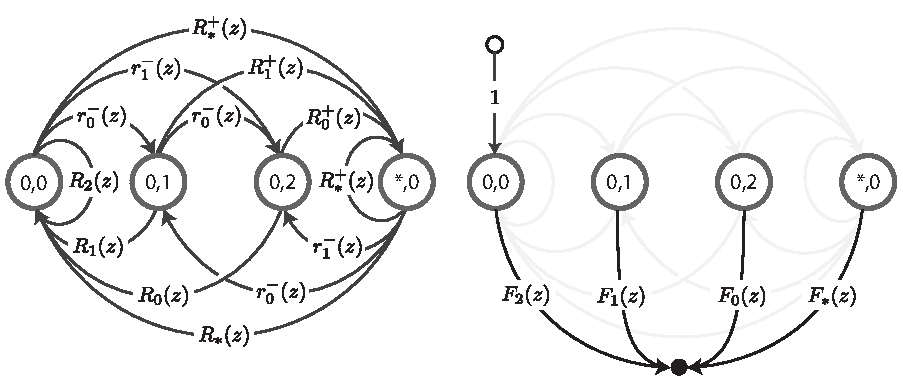
\includegraphics[scale=0.79]{MEM_graph.pdf}
\caption{\textbf{Transfer graph of reads without $3$-MEM seed for $(+)$}.
Text.}
\label{fig:graph_mem}
\end{figure}


By considering all the cases, we obtain the transfer graph shown in
figure~\ref{fig:graph_mem}. The numbers in the vertices indicate the
amount of nucleotides matching $(-)$ and $(+)$ at the end of the
$R$-blocks. Since $R$-blocks are terminated by a mismatch, at least one of
these numbers is $0$. As explained above, the $*$ symbol stands for one or
more nucleotides, as all these cases are equivalent. The body of the
transfer graph is represented on the left panel, the head and tail edges
on the right panel.

Simple $R$-blocks have weighted generating functions $r_0^+(z)$,
$r_0^-(z)$, $r_1^+(z)$ or $r_1^-(z)$. The sign indicates which sequence
is \emph{mismatched} at the end of the $R$-block and the index indicates
the number of matches in the $R$-block. Unions of $R$-blocks have weighted
generating functions $R_*(z)$, $R_*^+(z)$ or $R_i^+(z)$. The first
represents any number of matches followed by a double mismatch, the second
represents any number of matches followed by a mismatch against the $(+)$
sequence, the last represent \emph{up to} $i$ matches followed by a
mismatch against the $(+)$ sequence.

In the initial state of the read, the amount of matching nucleotides is
$(0,0)$, which is indicated by the label $1$ on the edge between the head
vertex and the vertex $(0,0)$. This is equivalent to prepending the read
by the empty object $\varepsilon$. Reads are terminated by a sequence of
matches. The weighted generating functions $F_*(z)$, $F_0(z)$, $F_1(z)$
and $F_2(z)$ represent mismatch-free intervals of any size or size
\emph{up to} $0$, $1$ or $2$, respectively. Here $\psi(z) = 0$. The empty
sequence is present in the graph (take a path from the head vertex to the
tail vertex through $(0,0)$ with no match appended at the tail), and no
extra sequence needs to be added.

The same logic can be applied for higher values of $\gamma$. The general
transfer matrix associated with the body of the transfer graph has
dimension $\gamma+1$ and is defined as


\begin{equation*}
M(z) =
\begin{blockarray}{ccccccc}
   & \scriptstyle{0,0} & \scriptstyle{0,1} & \scriptstyle{0,2}
   & \ldots & \scriptstyle{0,\gamma-1} & \scriptstyle{*,0} \\
\begin{block}{c[cccccc]}
\scriptstyle{0,0} & R_{\gamma-1}(z) &
    r_0^-(z) & r_1^-(z) & \ldots & r_{\gamma-2}^-(z) & R_*^+(z) \\
\scriptstyle{0,1} & R_{\gamma-2}(z) & 0 & r_0^-(z) &
    \ldots & r_{\gamma-3}^-(z) & R_{\gamma-2}^+(z) \\
\scriptstyle{0,2} & R_{\gamma-3}(z) & 0 & 0 &
    \ldots & r_{\gamma-4}^-(z) & R_{\gamma-3}^+(z)  \\
\vdots & \vdots & \vdots & \vdots & \ddots & \vdots & \vdots \\
\scriptstyle{0,\gamma-1} & R_0(z) & 0 & 0 & \ldots & 0 & R_0^+(z) \\
\scriptstyle{*,0} & R_*(z) &
    r_0^-(z) & r_1^-(z) & \ldots & r_{\gamma-2}^-(z) & R_*^+(z) \\
\end{block}
\end{blockarray}.
\end{equation*}


As per proposition~\ref{th:HBT}, the weighted generating function of reads
with no $\gamma$-MEM for the $(+)$ sequence is given by $H(z)^\top \cdot
(I-M(z))^{-1} \cdot T(z)$. In this case the head vector $H(z)$ is equal to
$(1,0,\ldots,0)^\top$ and the tail vector $T(z)$ is equal to
$(F_{\gamma-1}(z), \ldots, F_1(z), F_0(z), F_*(z))^\top$.

As in section~\ref{sec:fp}, denote $a$ the probability that the nucleotide
is a double match, $b$ that it is a mismatch against $(+)$, $c$ that it is
a mismatch against $(-)$ and $d$ that it is a mismatch for both. With
these definitions, expressions (\ref{eq:abcd}) still apply, and we also
have

\begin{equation*}
\begin{gathered}
R_*(z) = \big(1 + az + (az)^2 + \ldots \big)dz = \frac{dz}{1-az}, \\
R_*^+(z) = \big(1 + az + (az)^2 + \ldots \big)cz = \frac{cz}{1-az}, \\
R_i^+(z) = \big(1 + az + \ldots  + (az)^i\big)cz, \\
F_*(z) = 1 + az + (az)^2 + \ldots = \frac{1}{1-az}.
\end{gathered}
\end{equation*}


Knowing the values of $a$, $b$, $c$ and $d$, we can compute the weighted
generating function $H(z)^\top \cdot (I-M(z))^{-1} \cdot T(z)$ and use
proposition~\ref{th:ass} to obtain an asymptotic estimate of the
probability that a read does not contain a $\gamma$-MEM for the $(+)$
sequence.

We now return to the problem of finding the probablity that a read
contains a $\gamma$-MEM seed when the target sequence has exactly one
duplicate. If we consider that the $(+)$ sequence is the target and that
the $(-)$ sequence is the duplicate, the probability described above is
the one we are searching. The model is completely specified by the
substitution rates $p$ and $\kappa$, and as in section~\ref{sec:fp} $a =
(1-p)(1-\kappa)$, $b = p\kappa/3$, $c = (1-p)\kappa$ and $d =
p(1-\kappa/3)$. The example below shows how the computations are carried
out in practice.



\begin{example}
\label{ex:num6}
Let us approximate the probability that a read does not contain a MEM seed
(where the target has one duplicate) for a read of size $k=100$ with
$\gamma=17$ and for $p=0.10$ and $\kappa=0.10$. First, we substitute in
the $18 \times 18$ transfer matrix $M(z)$ and in $T(z)$ the values
$a=0.81, b=0.09, c=0.00333, d=0.09667$. We then compute the expression
$H(z)^\top \cdot (I-M(z))^{-1} \cdot T(z)$ and obtain a function
$P(z)/Q(z)$ where $P$ and $Q$ are polynomials of degree $35$ and $36$,
respectively. The root of $Q$ with smallest \textit{modulus} is the
dominant singularity $z_1$ of the weighted generating function. Using
numerical approaches, we find $z_1 \approx 1.0266331946$. We compute the
proportionality constant of proposition~\ref{th:ass} as $P(z_1)/Q'(z_1)
\approx 1.3893346$ from which we obtain the final estimate
$1.3893346/1.0266331946^{101} \approx 0.09769252$. For comparison, a 99\%
confidence interval obtained by performing 10 billion random simulations
is $0.097682-0.097698$.
% The magic number is 9023102236 out of 10 billion.
\end{example}

Figure~\ref{fig:simulp_mem} illustrates the precision of this estimate for
different values of the error rate $p$ and of the read size $k$. The
values of the parameters are chosen to match those of
figure~\ref{fig:simulp} where we used exact seeds. In the conditions
above, the seeding probabilities are alomst indistinguishable. This does
not mean that the cost of using MEM seeds is always negligible. When using
MEMs, the seeding probability goes down as the number of duplicates goes
up (here we assume that there is only one duplicate). In addition we are
not separating type I and type II errors, which typically have different
costs.

\begin{figure}[h]
\centering
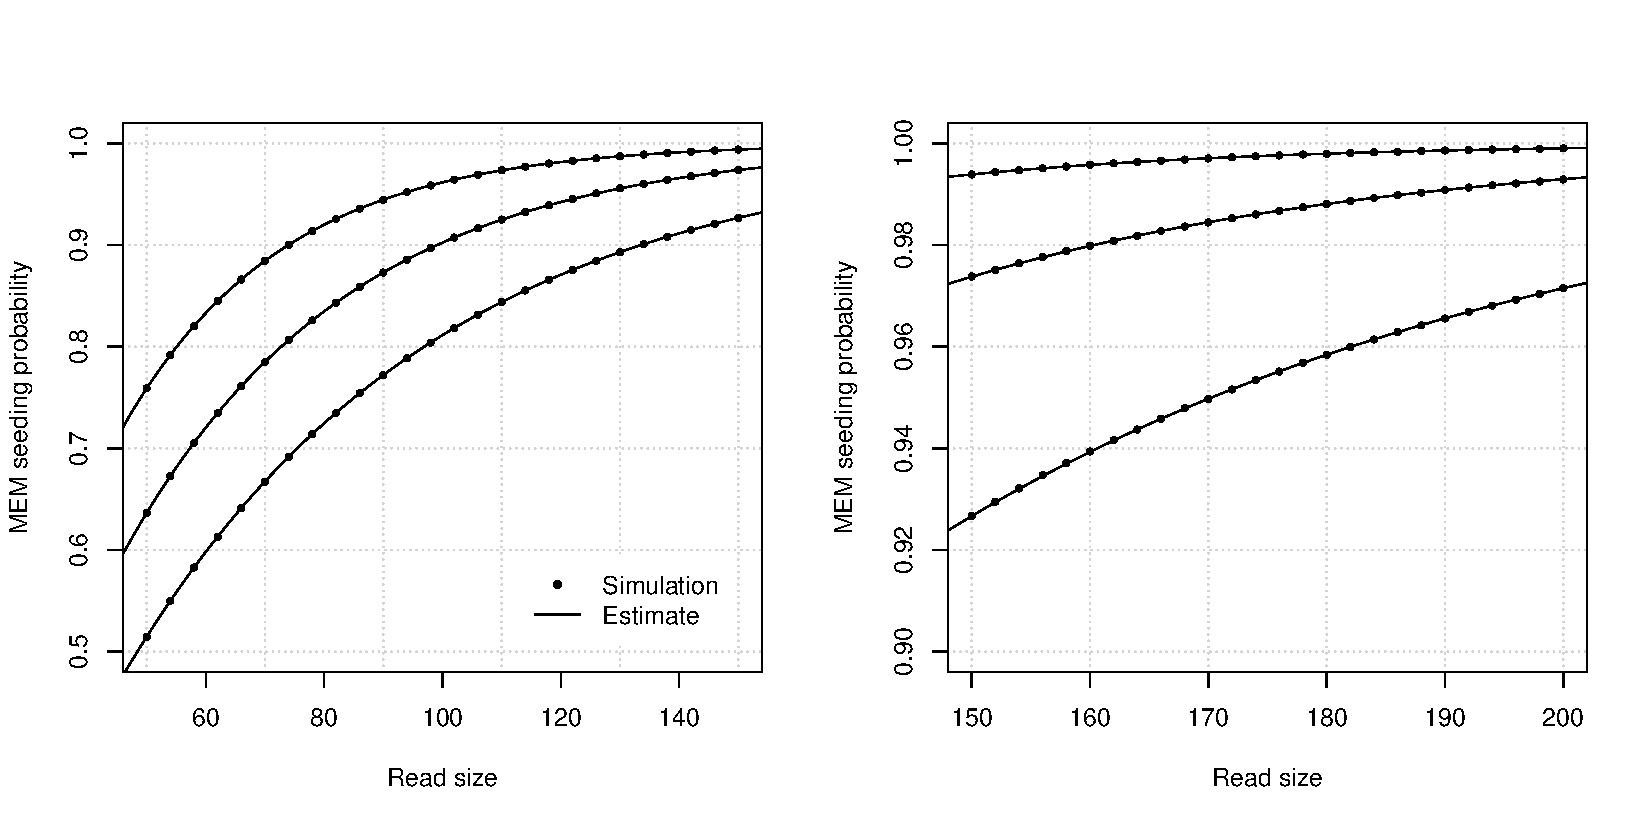
\includegraphics[scale=0.445]{simulp_mem.pdf}
\caption{\textbf{Example estimates of MEM seeding probability (one
duplicate)}. The analytic combinatorics estimates are benchmarked against
random simulations. Shown on both panels are the probablities that a read
of given size will contain a MEM seed, either estimated by 10,000,000
random simulations (dots), or by the method described above (lines). The
curves are drawn for $\gamma=17$ and $\kappa=0.10$, $p=0.08$, $p=0.10$ or
$p=0.12$ (from top to bottom). Notice how close the values are to those
shown in figure~\ref{fig:simulp} (probabilities that the read contains an
exact seed with the same parameter values).}
\label{fig:simulp_mem}
\end{figure}


This raises the question of how to compute the type I error rate when
using MEM seeds. The work above provides all the elements we need to
approximate it. Call the $P_3$ the approximate probability that the read
does not contain a $\gamma$-MEM seed. Using the results from
section~\ref{sec:fp}, we can compute an asymptotic estimate of the
probability that a read does not contain an exact $\gamma$-seed \emph{and}
does not contain any stretch of size $\gamma$ or greater matching the
duplicate sequence. We previously called this estimated probability $P_2$.
We can estimate the probability of type I errors as $P_3-P_2$.

Let us clarify the last statement. Call $A$ the event that the read has no
$\gamma$-MEM seed and $B$ the event that it does not contain an exact
$\gamma$-seed \emph{and} does not contain any stretch of size $\gamma$ or
greater matching the duplicate sequence. First observe that $B \subset A$
so $P(A \cap B^c) = P(A) - P(B)$. Then, $B^c$ is the event that the read
contains an exact $\gamma$-seed, a stretch of size $\gamma$ or greater
matching the duplicate sequence, or both. Another way to describe $B^c$ is
that ``some hit is found in the read''. So $A \cap B^c$ is the event that
``some hit is found, but it is not the target'', which is the definition
of a type I error. Since $P(A) \approx P_3$ and $P(B) \approx P_2$, the
probability of type I errors is indeed approximately equal to $P_3 - P_2$.

\begin{remark}
The rationale above shows that the probability of type II error with MEM
seeds is approximately equal to the probability $P_2$ computed at
section~\ref{sec:fp}.
\end{remark}


The example below shows the probabilities of type I errors are computed in
practice.


\begin{example}
\label{ex:num7}
Let us approximate the probability of type I error with MEM seeds (with
one duplicate) for a read of size $k=100$ with $\gamma=17$ and for
substitution rates $p=0.10$ and $\kappa=0.10$. In example~\ref{ex:num5} we
found $P_2 \approx 1.4032791/1.0272930245^{101}$ and in
example~\ref{ex:num6} we found $P_3 \approx 1.3893346/1.0266331946^{101}$.
The type I error rate is then approximately equal to $P_3 - P_2 \approx
0.00521934$. For comparison, a 99\% confidence interval obtained by
performing 10 billion random simulations is $0.0052166-0.0052203$.
% The magic number is 52184556 out of 10 billion.
\end{example}


Figure~\ref{fig:simulp_mem_fp} illustrates the precision of this estimate
for difference values of the substitution rate $\kappa$ and of the read
size $k$. The approximation is grossly inaccurate for $\kappa = 0.05$.
where it is even negative for reads under 40 nucleotides. The issue here
is slow convergence, as mentioned in section~\ref{sec:worst}. The dominant
singularity is approximately equal to $1.066122$, while the modulus of the
second and the third is approximately equal to $1.110296$. For $k \leq
40$, the contribution of the higher order singularities is not negligible;
using only the dominant singularity we obtain $P_3 \approx 0.158993$,
compared to $P_3 \approx 0.163655$ when using three singularities.

\begin{figure}[h]
\centering
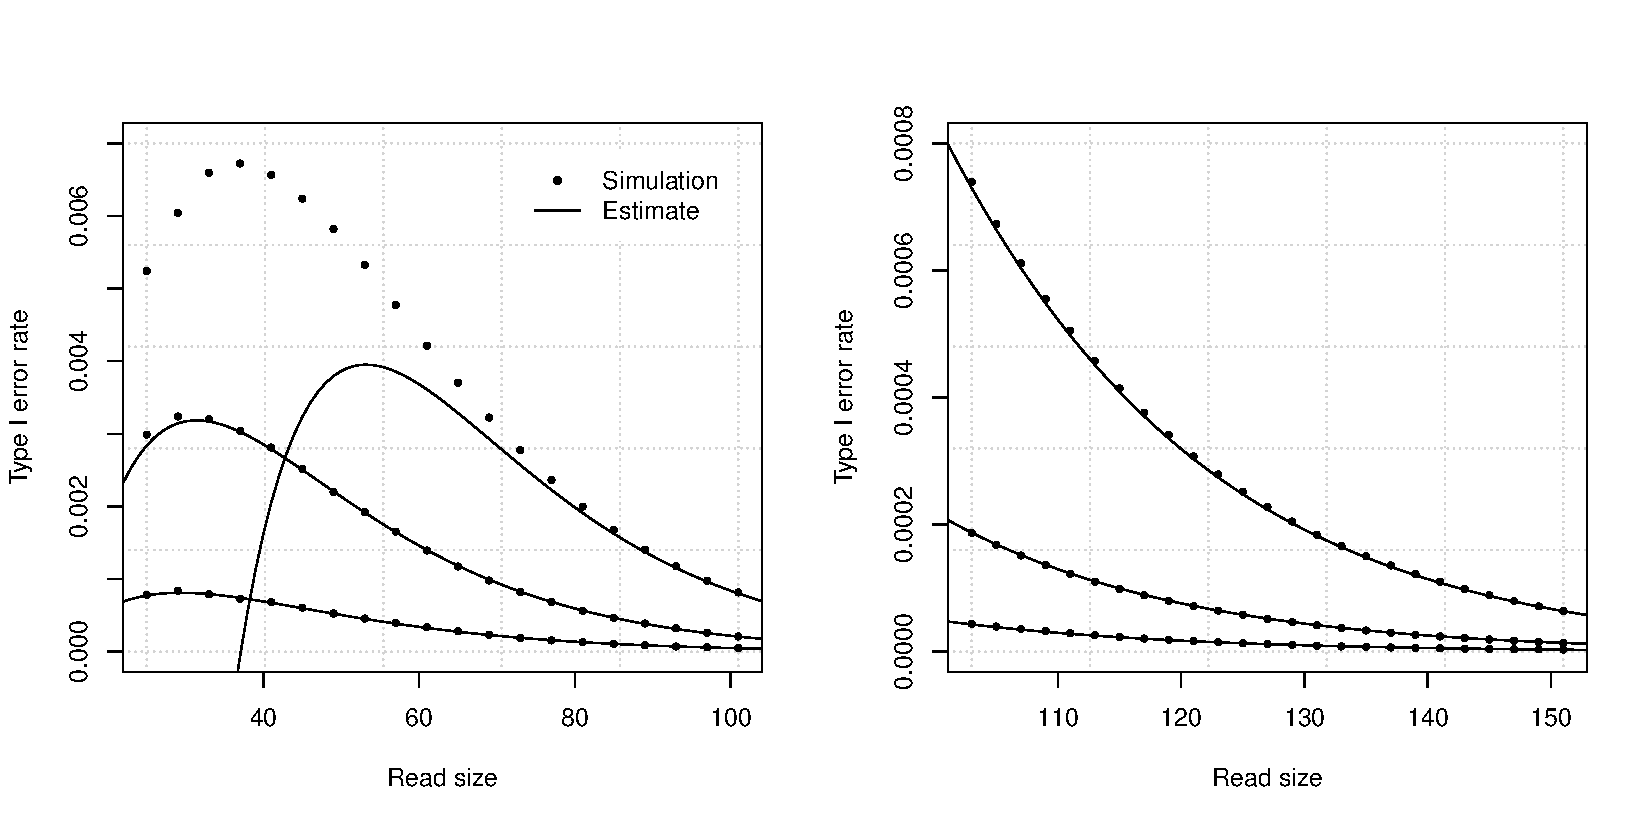
\includegraphics[scale=0.445]{simulp_mem_fp.pdf}
\caption{\textbf{Example estimates of MEM seeding probability (one
duplicate)}. The analytic combinatorics estimates are benchmarked against
random simulations. Shown on both panels are the probablities that a read
of given size will give a type I error when using MEM seeds, either
estimated by 10,000,000 (left) or 100,000,000 (right) random simulations
(dots), or by the method described above (lines). The curves are drawn for
$\gamma=17$ and $p=0.05$, $\kappa=0.05$, $\kappa=0.15$ or $\kappa=0.25$
(from top to bottom).}
\label{fig:simulp_mem_fp}
\end{figure}

Surprisingly, the estimations of $P_3$ in the cases $\kappa=0.15$ and
$\kappa=0.25$ are equally inacurate, but the errors almost perfectly
compensate with those on the approximation of $P_2$. Even more
surprisingly, using three singularities improves the approximations of
type I error rates for $\kappa=0.05$, but makes them worse for
$\kappa=0.15$ and $\kappa=0.25$ because the errors on $P_2$ and $P_3$ no
longer compensate. An emprirical solution is to record the $(p,\kappa)$
pairs for which to use one or three singularities. Even though this
solution is not satisfactory from the theoretical point of view, it gives
accurate approximations for the whole range of parameters, as shown in
figure~\ref{fig:simulp_mem_fp2}.


\begin{figure}[h]
\centering
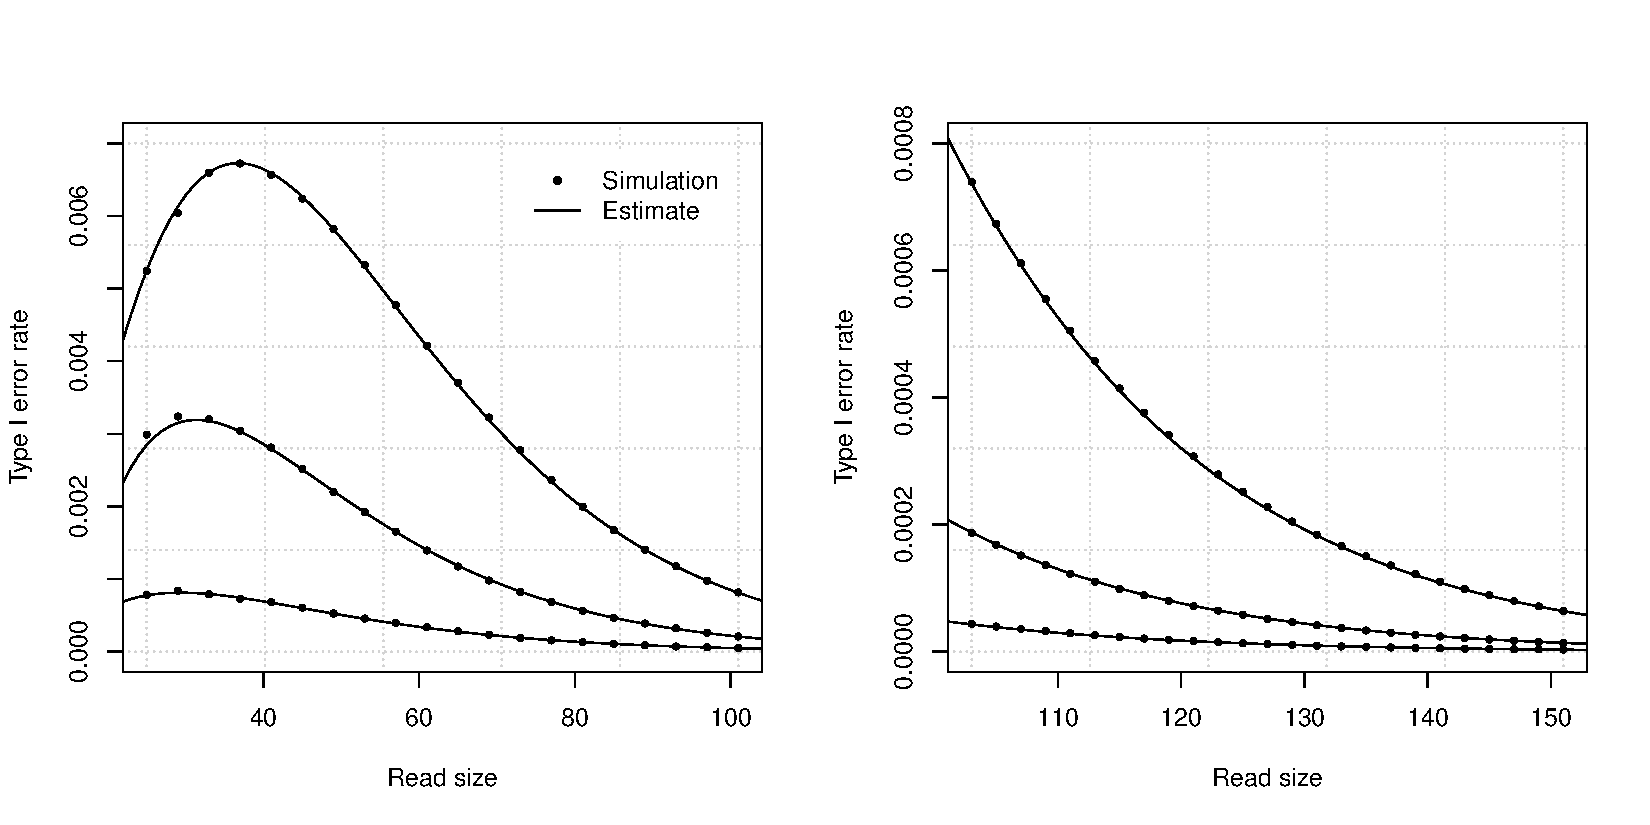
\includegraphics[scale=0.445]{simulp_mem_fp2.pdf}
\caption{\textbf{Example \textit{ad hoc} estimates of MEM seeding
probability (one duplicate)}. The analytic combinatorics estimates with
\textit{ad hoc} adjustments are benchmarked against random simulations.
Shown on both panels are the probablities that a read of given size will
give a type I error when using MEM seeds, either estimated by 10,000,000
(left) or 100,000,000 (right) random simulations (dots), or by the method
described above (lines). The curves are drawn for $\gamma=17$ and
$p=0.05$, $\kappa=0.05$, $\kappa=0.15$ or $\kappa=0.25$ (from top to
bottom). The simulation data points are the same as those shown in
figure~\ref{fig:simulp_mem_fp}. Three singularities are used to
approximate $P_3$ for $\kappa=0.05$, and only one for $\kappa=0.15$ and
$\kappa=0.25$.}
\label{fig:simulp_mem_fp2}
\end{figure}

We cannot use the method presented in section~\ref{sec:fp} to extend the
model to more than one duplicate because conditional independence does not
hold for MEM seeds. But we can still use the estimates above as a lower
bound for the probability of type I error. If the proportion of the genome
that is repeated is $x$ and $P^*$ is the maximum of $P_3-P_2$ relative to
unknown $\kappa$, then $xP^*$ is again a reasonable lower bound on the
probability of type I errors.




%%%%%%%%%%%%%%%%%% Average number of errors %%%%%%%%%%%%%%%%%%%%%
\section{Average quantities}
\label{sec:av}

\subsection{General approach}
\label{sec:genapp}


The analytic combinatorics approach allows computing the average of many
quantities of interest. In the seeding problem, one such quantity is the
number of errors for reads of different kinds. So far, weighted generating
functions only marked the size of the reads through the variable $z$. We
now need to introduce another variable to mark the second quantity, which
means that we will deal with bivariate weighted generating functions. For
concreteness, if $a_{k,n}$ is the total weight of seedless reads of size
$k$ and with $n$ errors, the average number of errors for reads of size
$k$ is by definition


\begin{equation}
\label{eq:av}
\left( \sum_{n=0}^\infty na_{k,n} \right) \Big/
 \left( \sum_{n=0}^\infty a_{k,n} \right).
\end{equation}

To compute this quantity, we introduce the variable $u$ marking the number
of substitutions and we write

\begin{equation*}
W(z,u) = \sum_{k=0}^\infty\sum_{n=0}^\infty a_{k,n}z^ku^n.
\end{equation*}

Finding an explicit formula for $W(z,u)$ is the focus of
sections~\ref{sec:avsub} to \ref{sec:avins}. For now, observe that
(\ref{eq:av}) can be expressed from $W(z,u)$ as follows. On the
one hand, we have

\begin{equation*}
W(z,1) = \sum_{k=0}^\infty \left( \sum_{n=0}^\infty a_{k,n} \right) z^k.
\end{equation*}

So the denominator of (\ref{eq:av}) is the coefficient of $z^k$ in
$W(z,1)$. On the other hand, by taking the derivative of $W(z,u)$ with
respect to $u$, and setting $u=1$, we obtain

\begin{equation*}
W_u(z,1) = \frac{\partial W(z,u)}{\partial u} \Bigr|_{\substack{\\u=1}} =
\sum_{k=0}^\infty \left( \sum_{n=0}^\infty na_{k,n} \right) z^k.
\end{equation*}

So the numerator of (\ref{eq:av}) is the coefficient of $z^k$ in
$W_u(z,1)$. Note that $W(z,1)$ and $W_u(z,1)$ are actually univariate
weighted generating functions, so we can use the methods developed earlier
to obtain asymptotic estimates for their coefficients. However,
proposition~\ref{th:ass} will not apply to approximate the coefficients of
$W_u(z,1)$. Since all the weighted generating functions considered here
are ratios of polynomials of the form $W(z,u) = P(z,u)/Q(z,u)$, the
derivative $W_u(z,1)$ can be expressed as $P_u(z,1)/Q(z,1) -
P(z,1)Q_u(z,1)/Q(z,1)^2$. Because of the term $Q(z,1)^2$ at the
denominator, the singularities of $W_u(z,1)$ are not simple poles.

Proposition~\ref{th:ass2} below shows how to extract the coefficients of
weighted generating functions in this particular case.




\begin{proposition}
\label{th:ass2}
If a function $W(z)$ is the ratio of two polynomials $P(z)/Q(z)^2$, and
$Q$ has only simple roots with distinct \textit{moduli}, then

\begin{equation}
\label{eq:ass2}
[z^k]W(z) \sim
\left( (k+1)\frac{P(z_1)}{z_1 Q'(z_1)^2} - \frac{P'(z_1)}{Q'(z_1)^2} +
\frac{P(z_1)Q''(z_1)}{Q'(z_1)^3} \right)
\frac{1}{z_1^{k+1}},
\end{equation}
where $z_1$ is the root of $Q$ with smallest \textit{modulus}.
\end{proposition}

As in proposition~\ref{th:ass}, we start by proving the lemma that will
give the functional expression of the asymptotic expansion.

\begin{lemma}
\label{lemma:poles2}
For $|z| < a$ we have

\begin{equation}
\label{eq:poles2}
\frac{1}{(1-z/a)^2} = \sum_{k=0}^\infty (k+1)\frac{z^k}{a^k}.
\end{equation}
\end{lemma}

\begin{proof}
\begin{equation*}
\frac{1}{(1-z/a)^2} = a \frac{\partial}{\partial z}
  \left( \frac{1}{1-z/a} \right)
= a \sum_{k=0}^\infty \frac{kz^{k-1}}{a^k},
\end{equation*}
where the last equality is obtained by differentiating after applying
lemma~\ref{lemma:poles}.
\end{proof}

We now prove proposition~\ref{th:ass2}.

\begin{proof}
As in the proof of proposition~\ref{th:ass}, let $z_1, z_2, \ldots, z_n$
be the complex roots of $Q$, sorted by increasing order of
\textit{modulus}. Since the roots of $Q(z)^2$ all have multiplicity 2,
there exists constants $\alpha_1, \ldots, \alpha_n$ and $\beta_1, \ldots,
\beta_n$ such that the partial fraction decomposition of the rational
function $P(z)/Q(z)^2$ can be written as

\begin{equation*}
\frac{P(z)}{Q(z)^2} = 
\sum_{j=1}^n \frac{\alpha_j}{(z-z_j)^2} + \frac{\beta_j}{z-z_j} =
\sum_{j=1}^n \frac{\alpha_j/z_j^2}{(1-z/z_j)^2}
-\frac{\beta_j/z_j}{1-z/z_j}.
\end{equation*}

As in the proof of proposition~\ref{th:ass}, we assumed without loss of
generality that the degree of $P$ is lower than the degree of $Q^2$. Now
applying lemmas~\ref{lemma:poles} and \ref{lemma:poles2}, we see that the
coefficient of $z^k$ in $P(z)/Q(z)^2$ can be expressed as

\begin{equation}
\label{eq:fullass2}
\sum_{j=1}^n (k+1)\frac{\alpha_j}{z_j^{k+2}}-\frac{\beta_j}{z_j^{k+1}}.
\end{equation}

The sum above is dominated by the term with the highest exponential rate
of increase, \textit{i.e.} $j=1$ because $z_1$ has smallest modulus by
definition. Thus, the coefficient of $z^k$ in $P(z)/Q(z)^2$ is
asymptotically equivalent to 

\begin{equation*}
(k+1)\frac{\alpha_1}{z_1^{k+2}}-\frac{\beta_1}{z_1^{k+1}}.
\end{equation*}

We now need to find the values of $\alpha_1$ and $\beta_1$. As $z_1$ is a
root of $Q$, there exists a polynomial $Q_1(z)$ such that

\begin{equation}
\label{eq:Q1}
Q(z) = (z-z_1)Q_1(z).
\end{equation}

We can thus write $P(z)/Q(z)^2$ as

\begin{equation}
\label{eq:misc1}
\frac{P(z)}{(z-z_1)^2Q_1(z)^2} = \frac{\alpha_1}{(z-z_1)^2} +
\frac{\beta_1}{z-z_1} +
\sum_{j=2}^n \frac{\alpha_j}{(z-z_j)^2} + \frac{\beta_j}{z-z_j}.
\end{equation}

Multiplying both sides of (\ref{eq:misc1}) by $(z-z_1)^2$ and setting $z =
z_1$ shows that $\alpha_1 = P(z_1)/Q_1(z_1)^2$. To find the value of
$Q_1(z_1)$ we differentiate (\ref{eq:Q1}) and let $z = z_1$, yielding
$Q'(z_1) = Q_1(z_1)$. We thus obtain $\alpha_1 = P(z_1) / Q'(z_1)^2$.

To find the value of $\beta_1$, we subtract $\alpha_1/(z-z_1)^2$ on both
sides of (\ref{eq:misc1}) and obtain

\begin{equation}
\label{eq:misc2}
\frac{P(z) - P(z_1)Q_1(z)^2/Q_1(z_1)^2}{(z-z_1)^2Q_1(z)^2} =
\frac{\beta_1}{z-z_1} + 
\sum_{j=2}^n \frac{\alpha_j}{(z-z_j)^2} + \frac{\beta_j}{z-z_j}.
\end{equation}

Since $P(z_1) - P(z_1)Q_1(z_1)^2/Q_1(z_1)^2 = 0$, there exists a
polynomial $Q_2(z)$ such that

\begin{equation}
\label{eq:Q2}
P(z) - P(z_1)Q_1(z)^2/Q_1(z_1)^2 = (z-z_1)Q_2(z).
\end{equation}


Multiplying (\ref{eq:misc2}) by $z-z_1$ and setting $z =
z_1$, we obtain $\beta_1 = Q_2(z_1)/Q_1(z_1)^2$. To find the value of
$Q_2(z_1)$ we differentiate (\ref{eq:Q1}) two times and (\ref{eq:Q2})
one time, finally obtaining
$\beta_1 = P'(z_1)/Q'(z_1)^2 - P(z_1)Q''(z_1)/Q'(z_1)^3$, which concludes
the proof.
\end{proof}


\begin{remark}
Expression (\ref{eq:ass2}) is asymptotically equivalent to the simpler
expression

\begin{equation}
\label{eq:ass3}
(k+1)\frac{P(z_1)}{Q'(z_1)^2}\frac{1}{z_1^{k+2}}.
\end{equation}

However, the convergence of expression (\ref{eq:ass3}) is slow. Indeed,
dividing the exact expression (\ref{eq:fullass2}) by (\ref{eq:ass3}) gives
an error term in $O(1/k)$. In comparison, dividing (\ref{eq:fullass2}) by
(\ref{eq:ass2}) gives an error term in $O(|z_1/z_2|^k)$, which decreases
exponentially, as in proposition~\ref{th:ass}.
\end{remark}


We are now ready to approximate the mean number of errors in reads of
different kinds. We treat the distinct types of errors separately, in the
framework of the corresponding error model from
section~\ref{sec:substitutions} to \ref{sec:insertions}.


\subsection{Substitutions}
\label{sec:avsub}

Applying a now familiar strategy, we write the generating function of
simple objects that we combine them into more complex objects. Recall from
section~\ref{sec:substitutions} that in the uniform substitution model,
the weighted generating function of substitutions is $pz$, where $p$ is
the error rate. In order to mark them with the variable $u$, we replace
$pz$ by $pzu$. For every subtitution, the power of $z$ increases by $1$,
so the size of the read increases by $1$. The power of $u$ also increases
by $1$ irrespective of the size, which allows us to mark the number of
substitutions.

We could derive the weighted generating function by the transfer matrix
method described in section~\ref{sec:substitutions}, but we can get an
immediate result by using equation (\ref{eq:Sp}), where we observed
that the weighted generating function of reads without exact seed can
be expressed as

\begin{equation}
\tag{\ref{eq:Sp}}
\frac{1+F_\gamma(z)}{1-pz(1+F_\gamma(z))}.
\end{equation}

Here the weighted generating function of substitutions appears explicitly
as $pz$. We can replace it by $pzu$ to obtain directly

\begin{equation}
\label{eq:Szu}
S(z,u) = \frac{1+F_\gamma(z)}{1-pzu\big( 1+F_\gamma(z) \big)}.
\end{equation}


$S(z,1)$ is simply the weighted generating function of seedless reads
derived in section~\ref{sec:substitutions}, and for which we already
know the coefficient asymptotics. So we already have the denominator of
(\ref{eq:av}). Now differentiating (\ref{eq:Szu}) with respect to $u$, we
obtain

\begin{equation}
\label{eq:dSdu}
\frac{\partial }{\partial u}
\left(\frac{1+F_\gamma(z)}{1-pzu\big( 1+F_\gamma(z) \big)}
\right) \Biggr|_{\substack{\\u=1}} = 
\frac{pz(1+F_\gamma(z))^2}{\big( 1 - pz(1+F_\gamma(z)) \big)^2}.
\end{equation}

As mentioned above, the form of the weighted generating function calls for
using proposition~\ref{th:ass2} (and not proposition~\ref{th:ass}). The
dominant singularity is the same for both the numerator and the
denominator of (\ref{eq:av}), so the terms in $z_1^{k+1}$ cancel out. What
remains is an expression of the form $C_1k + C_2$, where $C_1$ and $C_2$
are constants. In other words, the average number of substitutions in
reads without exact seed increases as an affine function of the size. We
make this result more accurate in the following proposition.


\begin{proposition}
\label{th:avsub}
Under the assumptions of the error model of
section~\ref{sec:substitutions}, the average number of substitutions in
seedless reads of size $k$ is asymptotically equivalent to

\begin{equation*}
\frac{(1-qz)(C_1(k+1) - C_2)}{1-(\gamma+1-\gamma qz_1)(qz_1)^\gamma},
\end{equation*}
with

\begin{gather*}
C_1 = 1-(qz_1)^\gamma, \text{ and} \\
C_2 = \frac{
\big(1-(2-(1-qz_1)\gamma^2+2\gamma)(qz_1)^\gamma+
(1+(1-qz_1)\gamma^2-2\gamma)(qz_1)^{2\gamma} \big)}
{1-(\gamma+1-\gamma qz_1)(qz_1)^\gamma},
\end{gather*}
and where $z_1$ is the only positive root of the polynomial
$1-pz(1+F_\gamma(z))$.
\end{proposition}

\begin{proof}
Apply proposition~\ref{th:ass2} to (\ref{eq:dSdu}), use
proposition~\ref{th:p} and simplify.
\end{proof}

\begin{remark}
The estimate obtained from (\ref{eq:ass3}) instead of (\ref{eq:ass2})
increases linearly with $k$. In this case, only the relative error
vanishes asymptotically. The absolute error remains constant.
\end{remark}


\begin{figure}[h]
\centering
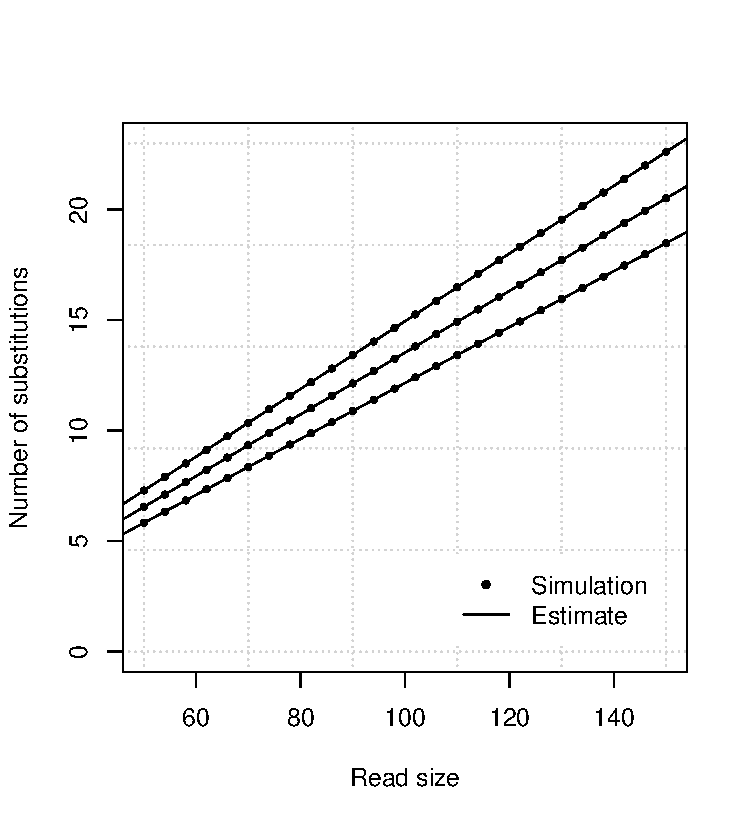
\includegraphics[scale=0.445]{simulp-average.pdf}
\caption{\textbf{Estimating the average number of substitutions}. The
average number of substitutions in reads without $\gamma$-exact seed is
shown for different read sizes, either estimated by 10,000,000 random
simulations (dots), or by analytic combinatorics (lines). The curves are
drawn for $\gamma=17$, $p=0.08$, $p=0.10$ or $p=0.12$ (from bottom to
top).}
\label{fig:simulavsub}
\end{figure}

Figure~\ref{fig:simulavsub} illustrates the accuracy of the estimate. The
affine relationshiop between the average number of errors and the size of
the read without exact seed is apparent, and the approximations are very
close to the target values.




\subsection{Deletions}
\label{sec:avdel}

To count the average number of deletions, we take the weighted generating
function of the reads without seed in the error model of
section~\ref{sec:deletions}, namely

\begin{equation}
\tag{\ref{eq:Sdel}}
\frac{1+(1-\delta)F_\gamma(z)}
  {1-pz - \big(pz(1-\delta) + \delta\big)F_\gamma(z)}.
\end{equation}

Here it is important to remember that for simplicity, equation
(\ref{eq:Sdel}) ignores the deletions that occur immediately before and
after substitutions, because they have no impact on the presence of a
seed. For the purpose of counting deletions, we need to take them all into
consideration, but this requires working with the proper weighted
generating function.

A read can be thought of as a walk on the graph shown in
figure~\ref{fig:deletions2}. Even though deletions appear as an explicit
state, their size is $0$ and they occur only between nucleotides (which
implies that a read can neither start nor end with a deletion). Also, a
deletion must be followed by either a match or a substitution; it cannot
be followed by a deletion. The reason is that a deletion has size $0$
regardless the number of deleted nucleotides. In the symbolic
representation of the read, either there is a deletion of any size between
two nucleotides, or there is no deletion.

\begin{figure}[h]
\centering
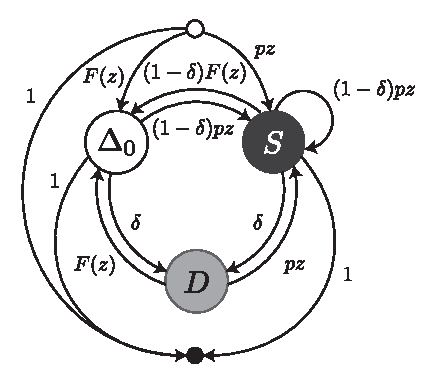
\includegraphics[scale=0.9]{deletions2.pdf}
\caption{\textbf{Transfer graph with explicit deletions}. 
Reads are viewed as sequences of error-free intervals (symbol $\Delta_0$)
or substitutions (symbol $S$) or deletions (symbol $D$), with respective
weighted generating functions $F(z)$, $pz$ and $\delta$.}
\label{fig:deletions2}
\end{figure}

Here, reads are sequences of error-free intervals withs symbol $\Delta_0$
and weighted generating function $F(z)$ or substitutions with symbol $S$
and weighted generating function $pz$, or deletions with symbol $D$ and
weighted generating function $\delta$. The only forbidden transitions in
the sequence are that two error-free intervals cannot follow each other
(together they form a single error-free interval) and two deletions cannot
follow each other (together they form a single deletion). In contrast with
figure~\ref{fig:deletions} where deletions do not have their own vertex,
we need to account for the absence of deletions in transitions between
error-free intervals and substitutions. This is done by prepending a
weight equal to $(1-\delta)$.

As in the previous section, in order to count deletions with parameter $v$
we their weigted generating function by $\delta v$. For every deletion the
power of $v$ increases by $1$ (and the power of $z$ remains the same).
This allows us to mark the number of deletions. The transfer matrix then
becomes a function of $z$, marking the size of the reads, and of $v$,
marking the number of deletions. The final expression of the transfer
matrix is



\begin{equation*}
M(z,v) = 
\begin{blockarray}{cccc}
       & \smDELz & \smS & \smD \\
\begin{block}{c[ccc]}
\smDELz & 0              & (1-\delta)pz & \delta v \\
\smS    & (1-\delta)F(z) & (1-\delta)pz & \delta v \\
\smD    & F(z)           & pz           & 0        \\
\end{block}
\end{blockarray}.
\end{equation*}

Recall that reads can neither start nor end by a deletion because they are
undetectable at those positions. Thus the head vector is $H(z,v) = (F(z),
pz, 0)^\top$ and the tail vector is $T(z,v) = (1,1,0)^\top$. The only
sequence we need to add is the empty sequence $\varepsilon$, so $\psi(z,v)
= 1$. Following proposition~\ref{th:HBT}, the weighted generating function
$S(z,v)$ is equal to $\psi(z,v) + H(z,v)^\top \cdot (I-M(z,v))^{-1} \cdot
T(z,v)$.

Following the general strategy to count average quantities, we first
compute $S(z,1)$. Naturally, we obtain expression (\ref{eq:Sdel}), which
is the weighted generating function of reads without exact seed. We also
differentiate $S(z,v)$ with respect to $v$ and let $v=1$ to obtain

\begin{equation}
\label{eq:full_deletions}
S_v(z,1) =
\frac{\delta\big( pz(1+(1-\delta)F_\gamma(z))+F_\gamma(z) \big)^2}
{\big( 1-pz - \big(pz(1-\delta) + \delta\big)F_\gamma(z) \big)^2}.
\end{equation}

As in the section~\ref{sec:avsub}, we derive the asymptotics by applying
proposition~\ref{th:ass2} to (\ref{eq:full_deletions}) and by applying
proposition~\ref{th:ass} to (\ref{eq:Sdel}). The terms $z_1^{k+1}$ cancel
out when computing the ratio as per equation (\ref{eq:av}), so the number
of deletions in reads without seed is asymptotically affine, \textit{i.e.}
of the form $C_1k+C_2$, where $C_1$ and $C_2$ are constants. In both
cases, $C_1$ and $C_2$ have cumbersome expressions, but they are easy to
compute from propositions~\ref{th:ass} and \ref{th:ass2}.

\begin{figure}[h]
\centering
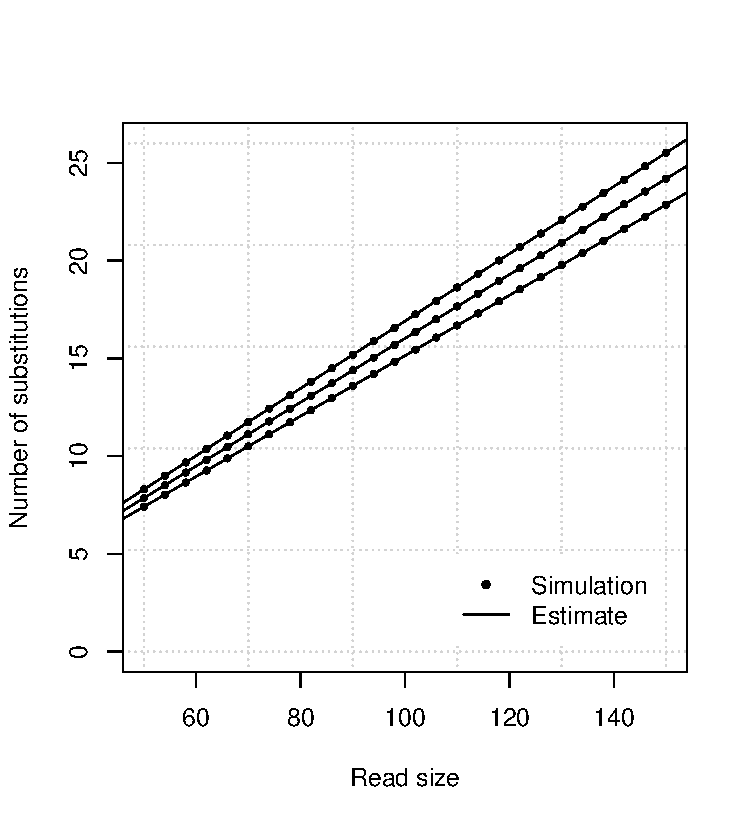
\includegraphics[scale=0.445]{simuldel-average2.pdf}
\caption{\textbf{Example estimates of average number of deletions}. The
average number of deletions in reads without $\gamma$-exact seed is
shown for different read sizes, either estimated by 10,000,000 random
simulations (dots), or by analytic combinatorics (lines). The curves are
drawn for $\gamma=17$, $p=0.05$ and $\delta=0.14$, $\delta=0.15$ or
$\delta=0.16$ (from bottom to top).}
\label{fig:simulavdel}
\end{figure}

The accuracy of the estimates is illustrated in
figure~\ref{fig:simulavdel}. Once again the affine relationship is a good
fit and the approximations are close the target values.





\subsection{Insertions}
\label{sec:avins}

Finally, we compute the average amount of insertions for reads without
exact seed in the full error model of section~\ref{sec:insertions}. The
simplest way to do this is to mark insertions directly in the transfer
matrix where they appear explicitly. For this, we append the extra
variable $w$ to their weighted generating functions and obtain the
following transfer matrix

\begin{equation*}
M(z,w) = 
\begin{blockarray}{cccc}
       & \smDELz & \smS & \smI \\
\begin{block}{c[ccc]}
\smDELz & \; \delta F_\gamma(z) & pz & rzw \; \\
\smS    & \;        F_\gamma(z) & pz & rzw \; \\
\smI    & \; (1-\tilde{r})F_\gamma(z)
           & (1-\tilde{r})pz & \tilde{r}zw \; \\
\end{block}
\end{blockarray}.
\end{equation*}

In the expression above, we have used $F_\gamma(z)$ instead of $F(z)$
because we are directly considering reads without seed. We also update the
head and tail vectors $H(z,w) = (F_\gamma(z), pz, rzw)^\top$ and
$T(z,w)=(1,1,1)^\top$, and we add the empty sequence, which does not
contain any insertion, so $\psi(z,w) = 1$. Following
proposition~\ref{th:HBT}, $S(z,w) = \psi(z,w) + H(z,w)^\top \cdot
(I-M(z,w))^{-1} \cdot T(z,w)$.

As explained in section~\ref{sec:genapp}, we obtain the average number of
insertions by computing ratio (\ref{eq:av}) from the coefficients of
$S(z,1)$ and of $S_w(z,1)$. Computing $S(z,1)$ yields expression
(\ref{eq:Sindel}), \textit{i.e.} the weighted generating function of reads
without exact seed. By differentiating $S(z,w)$ and setting $w=1$ we find
$S_w(z,1)$ to be equal to

\begin{equation}
\label{eq:full_insertions}
\frac{rz\big(1+(1-\delta)F_\gamma(z)\big)
\big(1-\tilde{r}pz+(1-\delta-\tilde{r}-(1-\delta)\tilde{r}pz)
  F_\gamma(z)\big)}
  {\big(1-a(z)-b(z)F_\gamma(z)\big)^2},
\end{equation}
where $a(z)$ and $b(z)$ are defined as in (\ref{eq:a+b}).

As in the section~\ref{sec:avsub}, we derive the asymptotics by applying
proposition~\ref{th:ass2} to (\ref{eq:full_insertions}) and by applying
proposition~\ref{th:ass} to (\ref{eq:Sindel}). The terms $z_1^{k+1}$ cancel
out when computing the ratio as per equation (\ref{eq:av}), so the number
of insertions in reads without seed is asymptotically affine,
\textit{i.e.} of the form $C_1k+C_2$, where $C_1$ and $C_2$ are constants.
In both cases, $C_1$ and $C_2$ have cumbersome expressions, but they are
easy to compute from propositions~\ref{th:ass} and \ref{th:ass2}.

\begin{figure}[h]
\centering
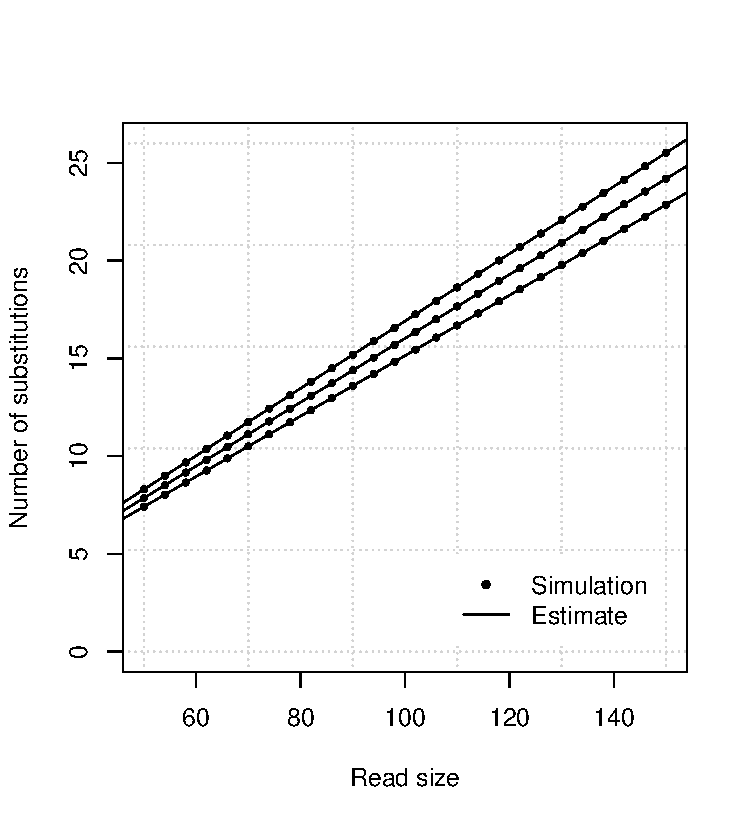
\includegraphics[scale=0.445]{simuldel-average2.pdf}
\caption{\textbf{Example estimates of average number of deletions}. The
average number of deletions in reads without $\gamma$-exact seed is
shown for different read sizes, either estimated by 10,000,000 random
simulations (dots), or by analytic combinatorics (lines). The curves are
drawn for $\gamma=17$, $p=0.05$ and $\delta=0.14$, $\delta=0.15$ or
$\delta=0.16$ (from bottom to top).}
\label{fig:simulavins}
\end{figure}

The accuracy of the estimates is illustrated in
figure~\ref{fig:simulavins}. Once again the affine relationship is a good
fit and the approximations are close the target values.


COMMENT ABOUT THE AVERAGE NUMBER OF ERRORS IN READS WITH SEED.



\section{Conclusion}

This concludes our introductory tour of the applications of analytic
combinatorics to seeding methods. There is of course much more to say. Our
purpose here is to show how the general strategy of analytic combinatorics
gives reasonable solutions to problems that were previously difficult to
address.

When using exact seeds, inexact seeds or MEM seeds, the estimates of the
seeding probabilities are robust and relatively straightforward. The data
collected during the alignment can be used to estimates the parameters of
the error model to auto-tune the seeding heuristic during the run. This
gives tight control of the type II error rate. More challenging is to
control the type I error rate. The estimates show some numeric instability
when using MEM seeds, but the real difficulty is the lack of theoretical
background on the seeding process when the target is duplicated.
Significant progress on this line may not come from analytic
combinatorics, but from more appropriate data structures or algorithms to
seed such sequences more efficiently.

Seeding is not only used in mapping, but also in other alignment problems.
In this regard, the work presented above can be applied to different
contexts. That said, mapping high throughput sequencing reads is a ``sweet
spot'' for analytic combinatorics because the sequences are long enough
for the approximations to be accurate.

Finally, the concepts developed above can also be used to sample reads of
different kinds. The analagoy between reads and walks on graphs with
weighted edges allows us to generate reads by simulating a random walk.
The trick is to convert the transfer matrix into a transition matrix by
using the weights of the objects as their probabilities of occurrence.

In summary, analytic combinatorics is a powerful strategy that comes with
a rich toolbox with many applications in modern bioinformatics. We expect
more applications to see the light as new algorithms and new heuristics
are developed in the future.





%---------------------------------------------------------------
%---------------------------------------------------------------

\bibliography{pubmed,extra}
\bibliographystyle{plain}

%----------------------------------------------------------------

\end{document}

%gs -dNoOutputFonts -sDEVICE=pdfwrite -o out.pdf latex.pdf 
